\chapter{Work Environments}

Block programming languages are a subdivision of visual programming languages. The essence of block languages is that program instructions are entered in the form of colored blocks and not, as in classical programming languages, by writing text commands. The most basic purpose of block languages is to make the field of programming significantly more accessible to beginners. This goal is achieved through three main directions. From a syntactic point of view, instructions in block languages are in the form of colored icons. This greatly reduces the possibility of writing the wrong program instruction. Second, semantics are improved, with each possible program instruction being well documented. In third place is pragmatism, which allows the study of the different states in which the program can fall. Block programming environments have grown in popularity over the past decade. Some of the most popular ones are Scratch, Blockly, App Inventor for Android, Ardublock, and others. This book will focus on two block programming environments created at MIT, Scratch and App Inventor for Android. This choice is because Scratch is aimed at the youngest, namely children in primary school classes, which is very well combined with the possibility to visualize the block programs on a mobile phone through App Inventor for Android. Both software environments do not require the installation of specialized software. It is enough to have a modern computer connected to the Internet and a modern web browser version.

\section{Getting Started in Scratch}

Working in the Scratch environment begins by loading the main web page (Fig. \ref{fig010001}), which is located at: \\ \href{https://scratch.mit.edu/}{https://scratch .mit.edu/}

\begin{figure}[H]
   \centering
   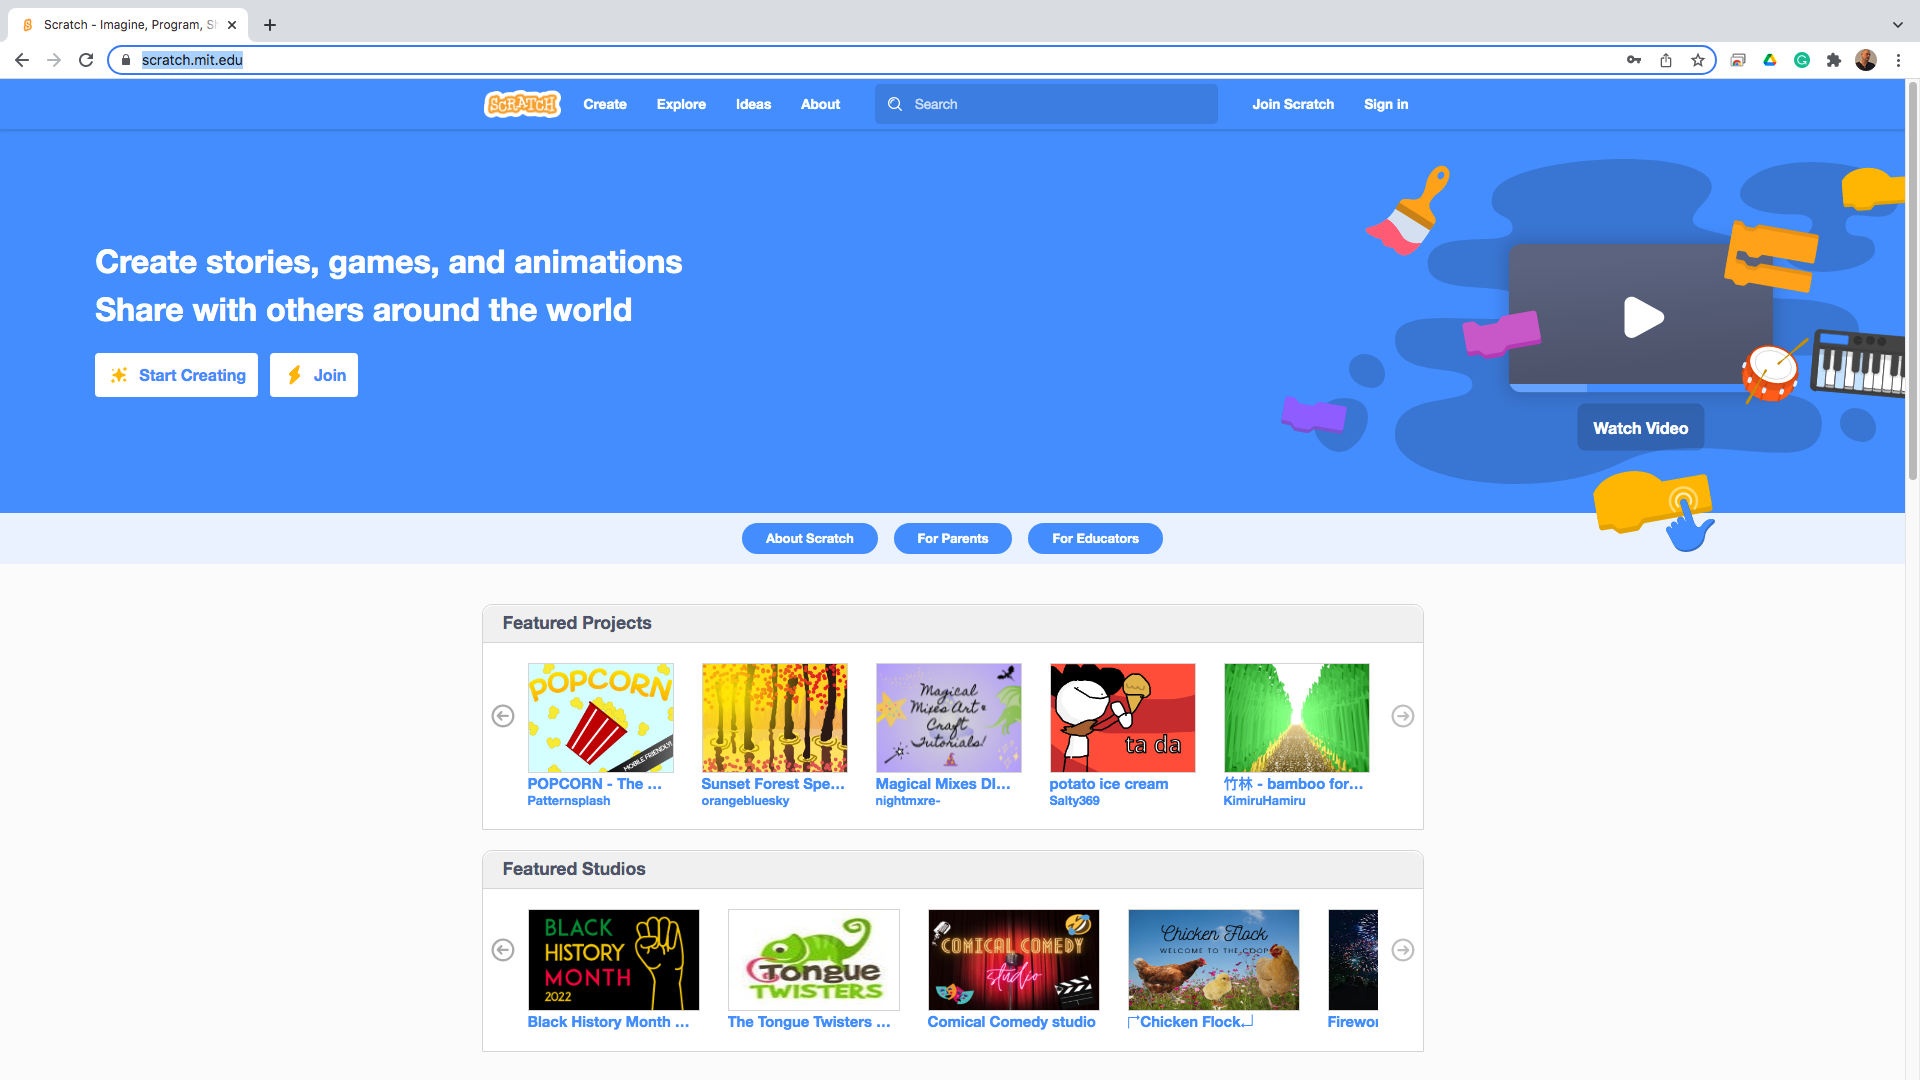
\includegraphics[width=1.0\linewidth,height=0.5\linewidth]{fig010001.png}
   \caption{Sratch Homepage}
\label{fig010001}
\end{figure}

The program environment of Sratch is organized on the principle of cloud services. For this reason, anyone wishing to use the service must register (Fig. \ref{fig010002}). The registration consists of a username and password.

\begin{figure}[H]
   \centering
   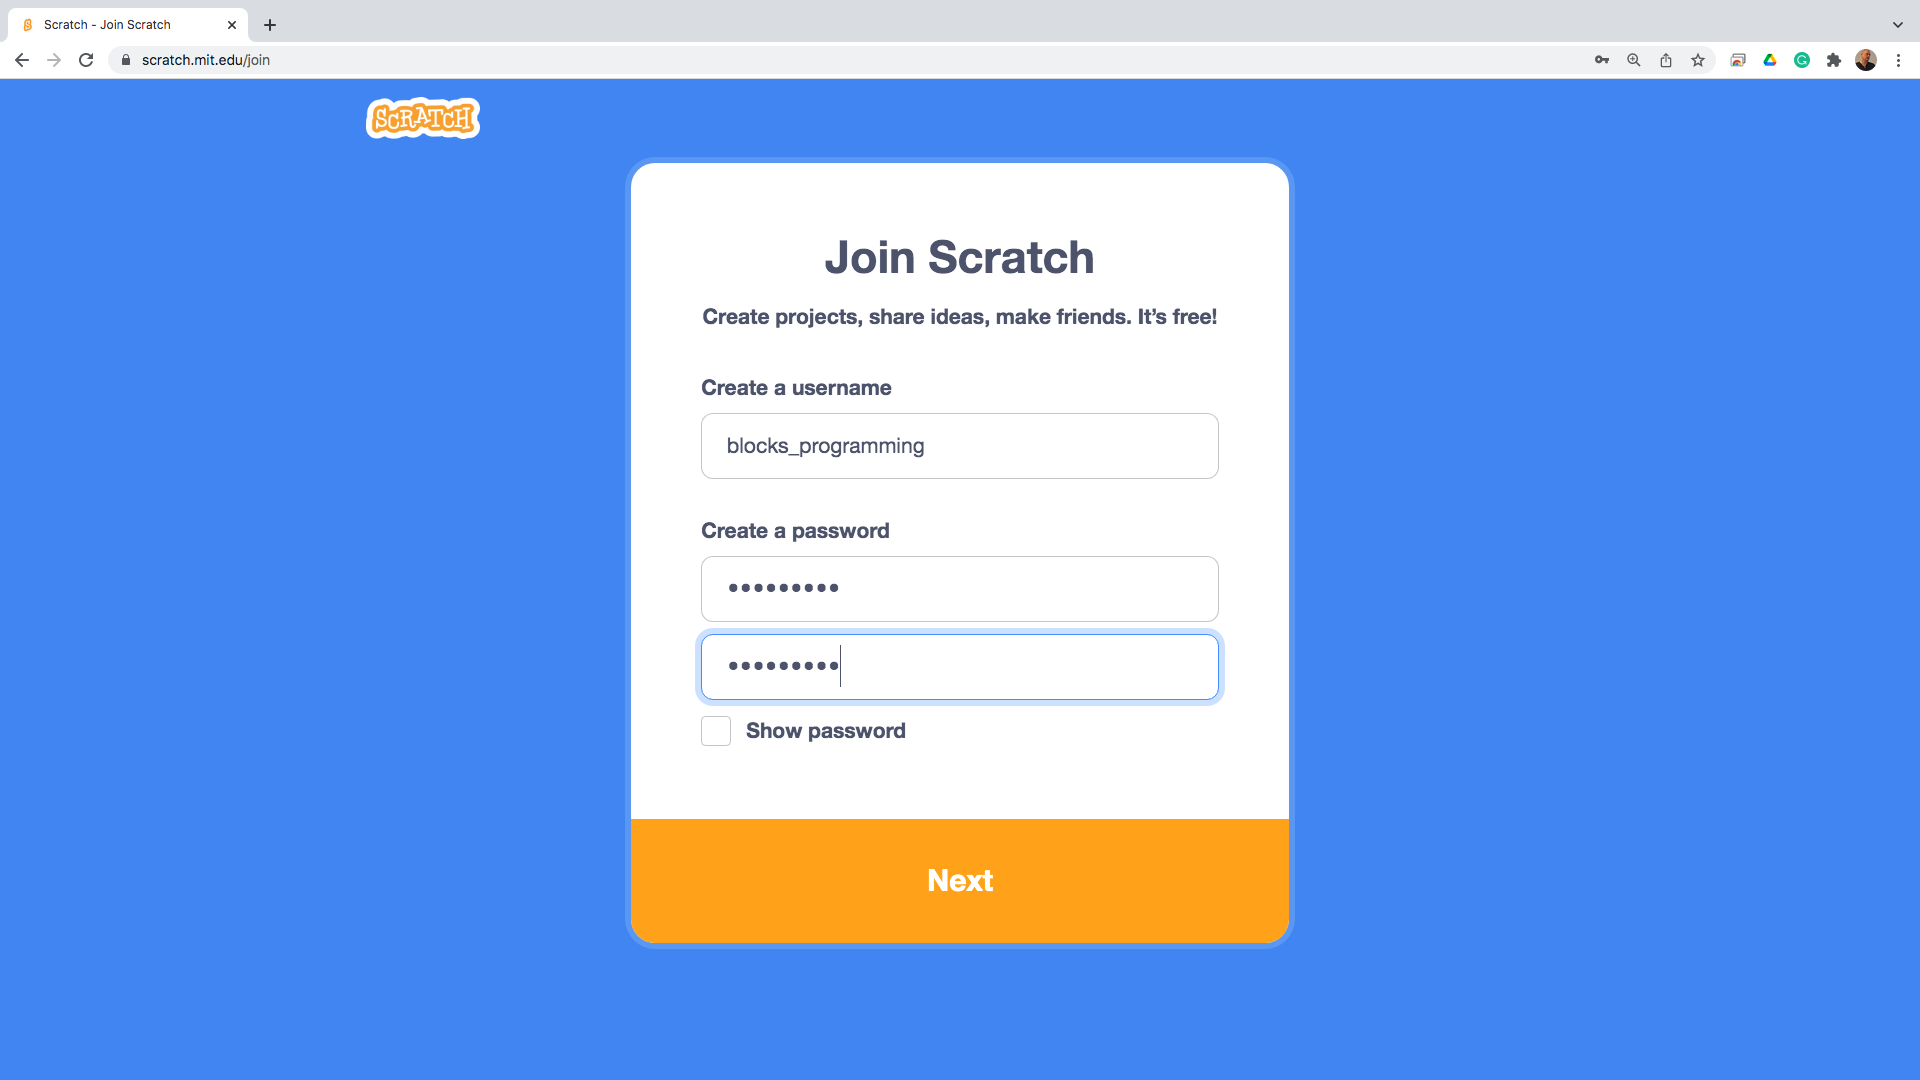
\includegraphics[width=1.0\linewidth,height=0.5\linewidth]{fig010002.png}
   \caption{Sratch user registration}
\label{fig010002}
\end{figure}

After choosing a username and password, the geographical region in which the user is located follows (Fig. \ref{fig010003}).

\begin{figure}[H]
   \centering
   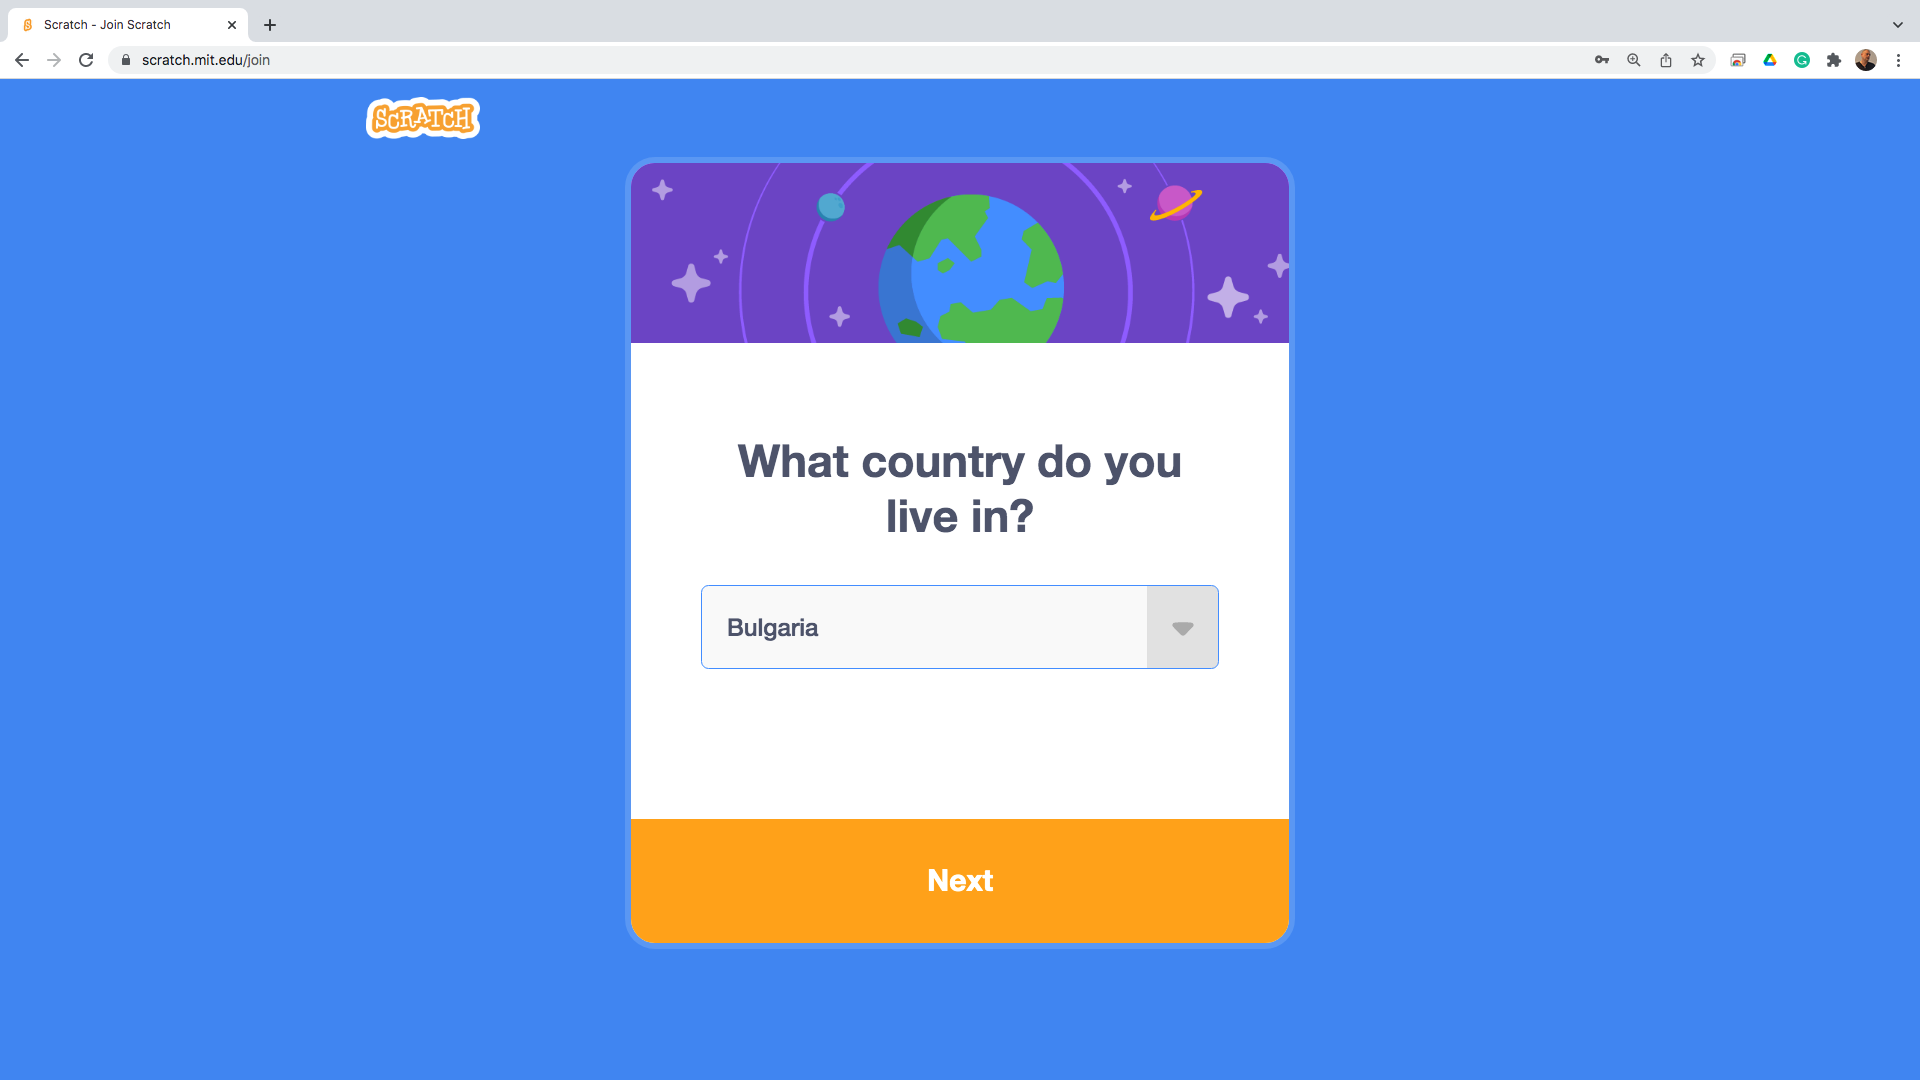
\includegraphics[width=1.0\linewidth,height=0.5\linewidth]{fig010003.png}
   \caption{Geographic location}
\label{fig010003}
\end{figure}

The platform is aimed primarily at children expressing an interest in programming but also at parents and teachers. For this reason, the system collects information about the user's age (Fig. \ref{fig010004}).

\begin{figure}[H]
   \centering
   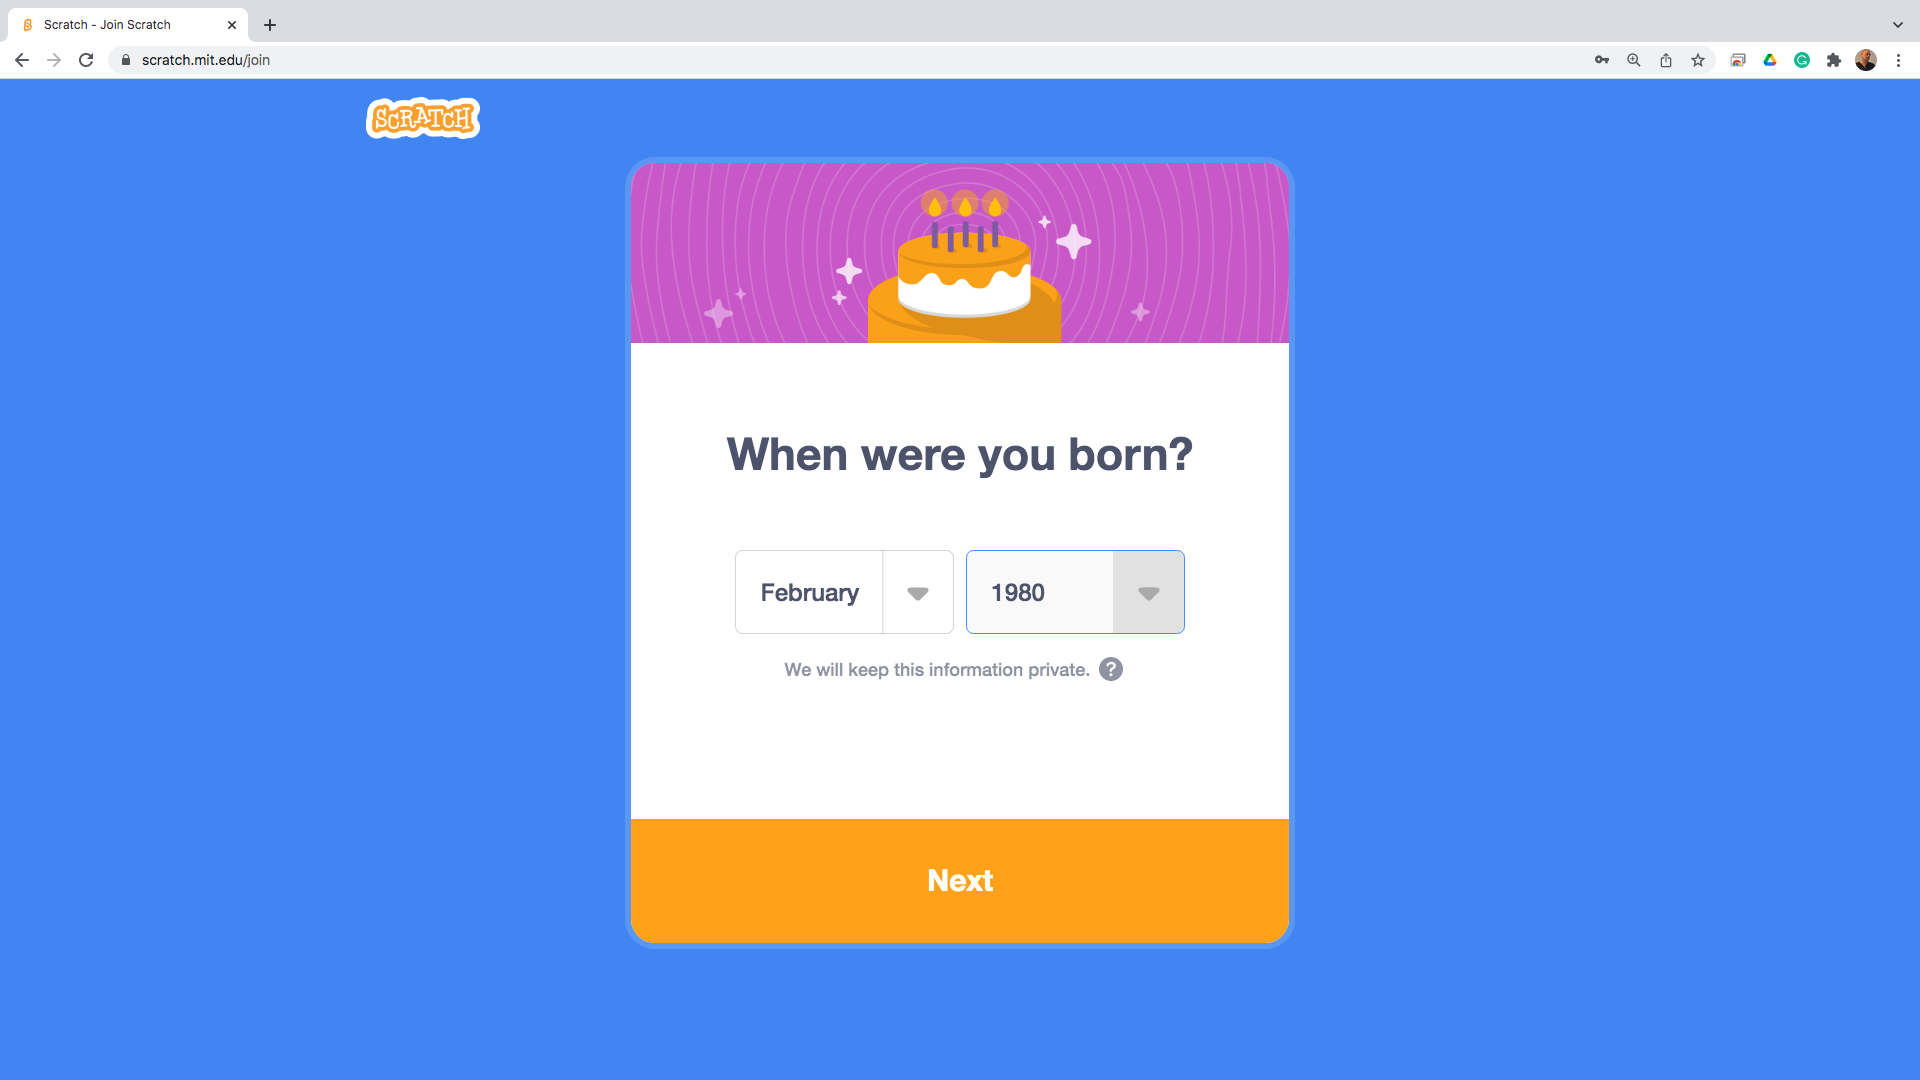
\includegraphics[width=1.0\linewidth,height=0.5\linewidth]{fig010004.png}
   \caption{Age of user}
\label{fig010004}
\end{figure}

In addition to classification by age, the system also collects information on type by gender. This information is optional to avoid discrimination (Fig. \ref{fig010005}).

\begin{figure}[H]
   \centering
   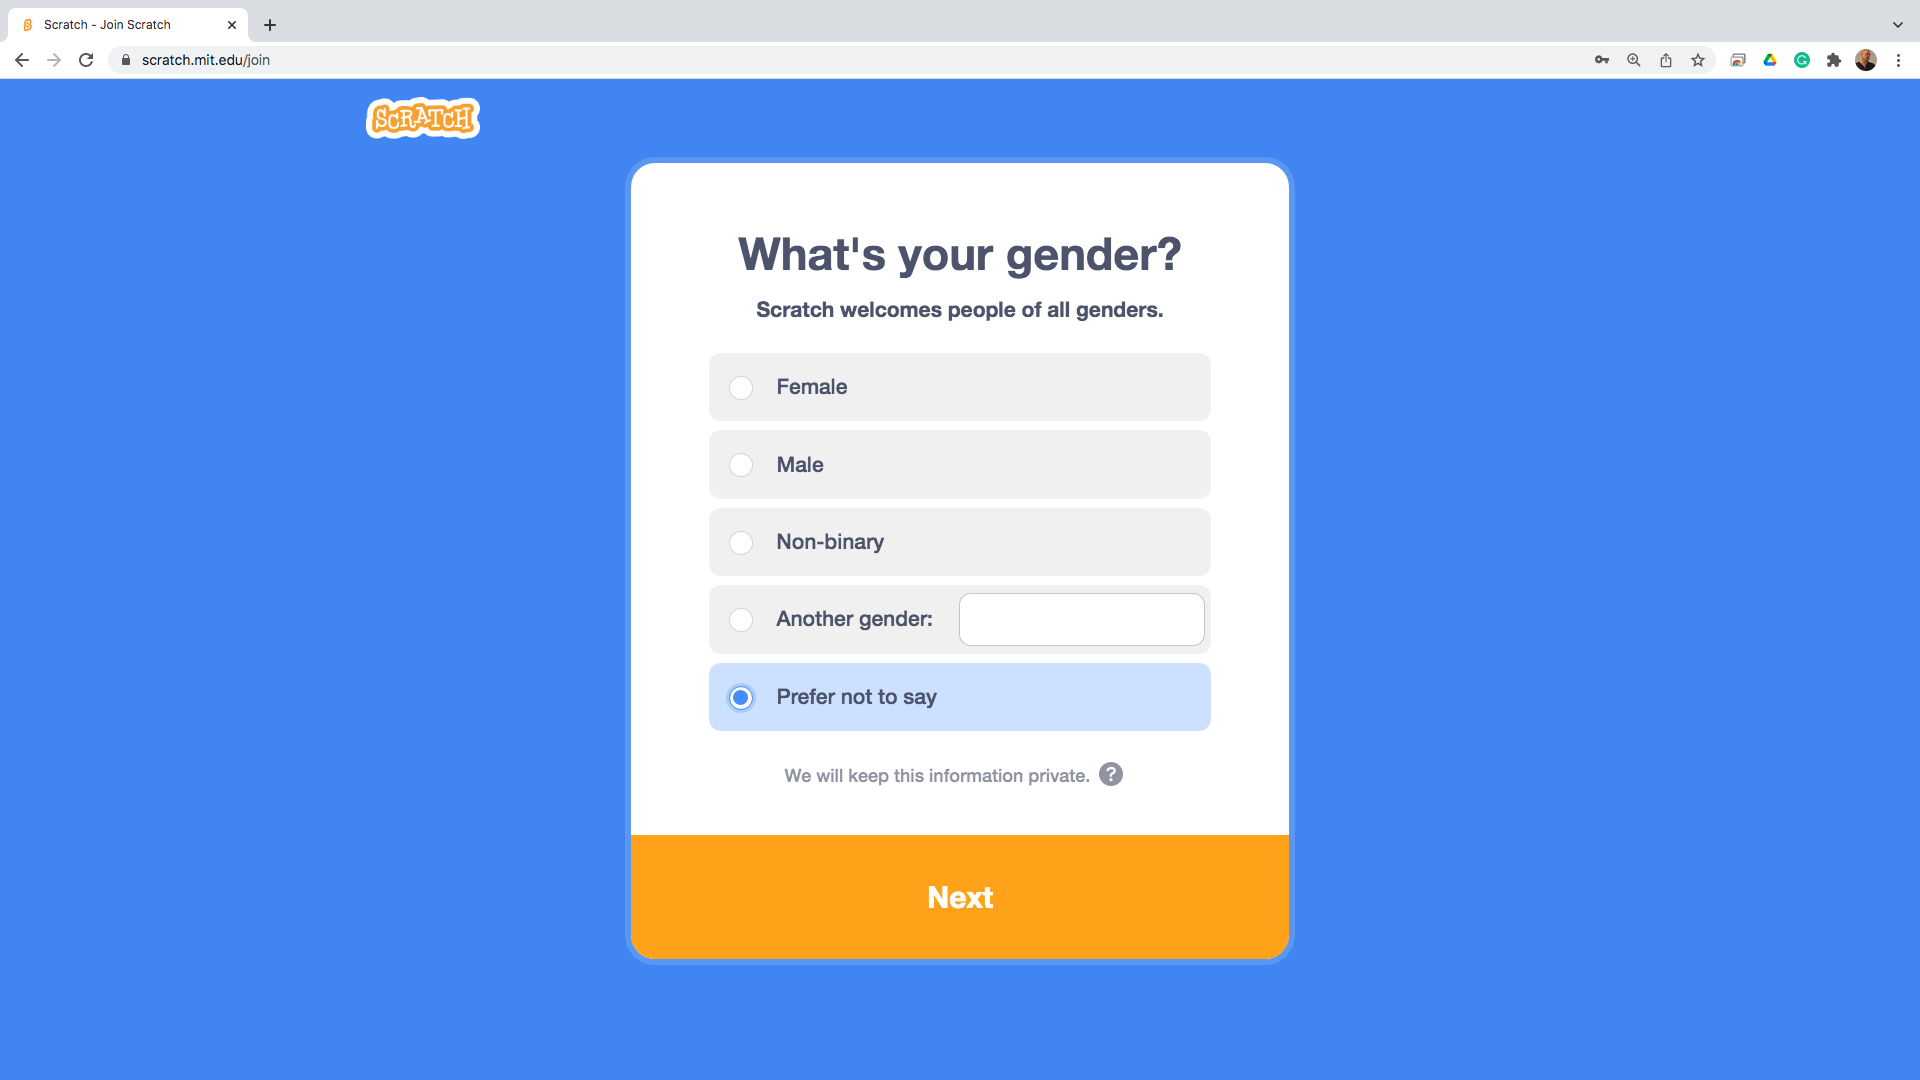
\includegraphics[width=1.0\linewidth,height=0.5\linewidth]{fig010005.png}
   \caption{User gender}
\label{fig010005}
\end{figure}

The user profile, username, and password must also be associated with an email address (Fig. \ref{fig010006}).

\begin{figure}[H]
   \centering
   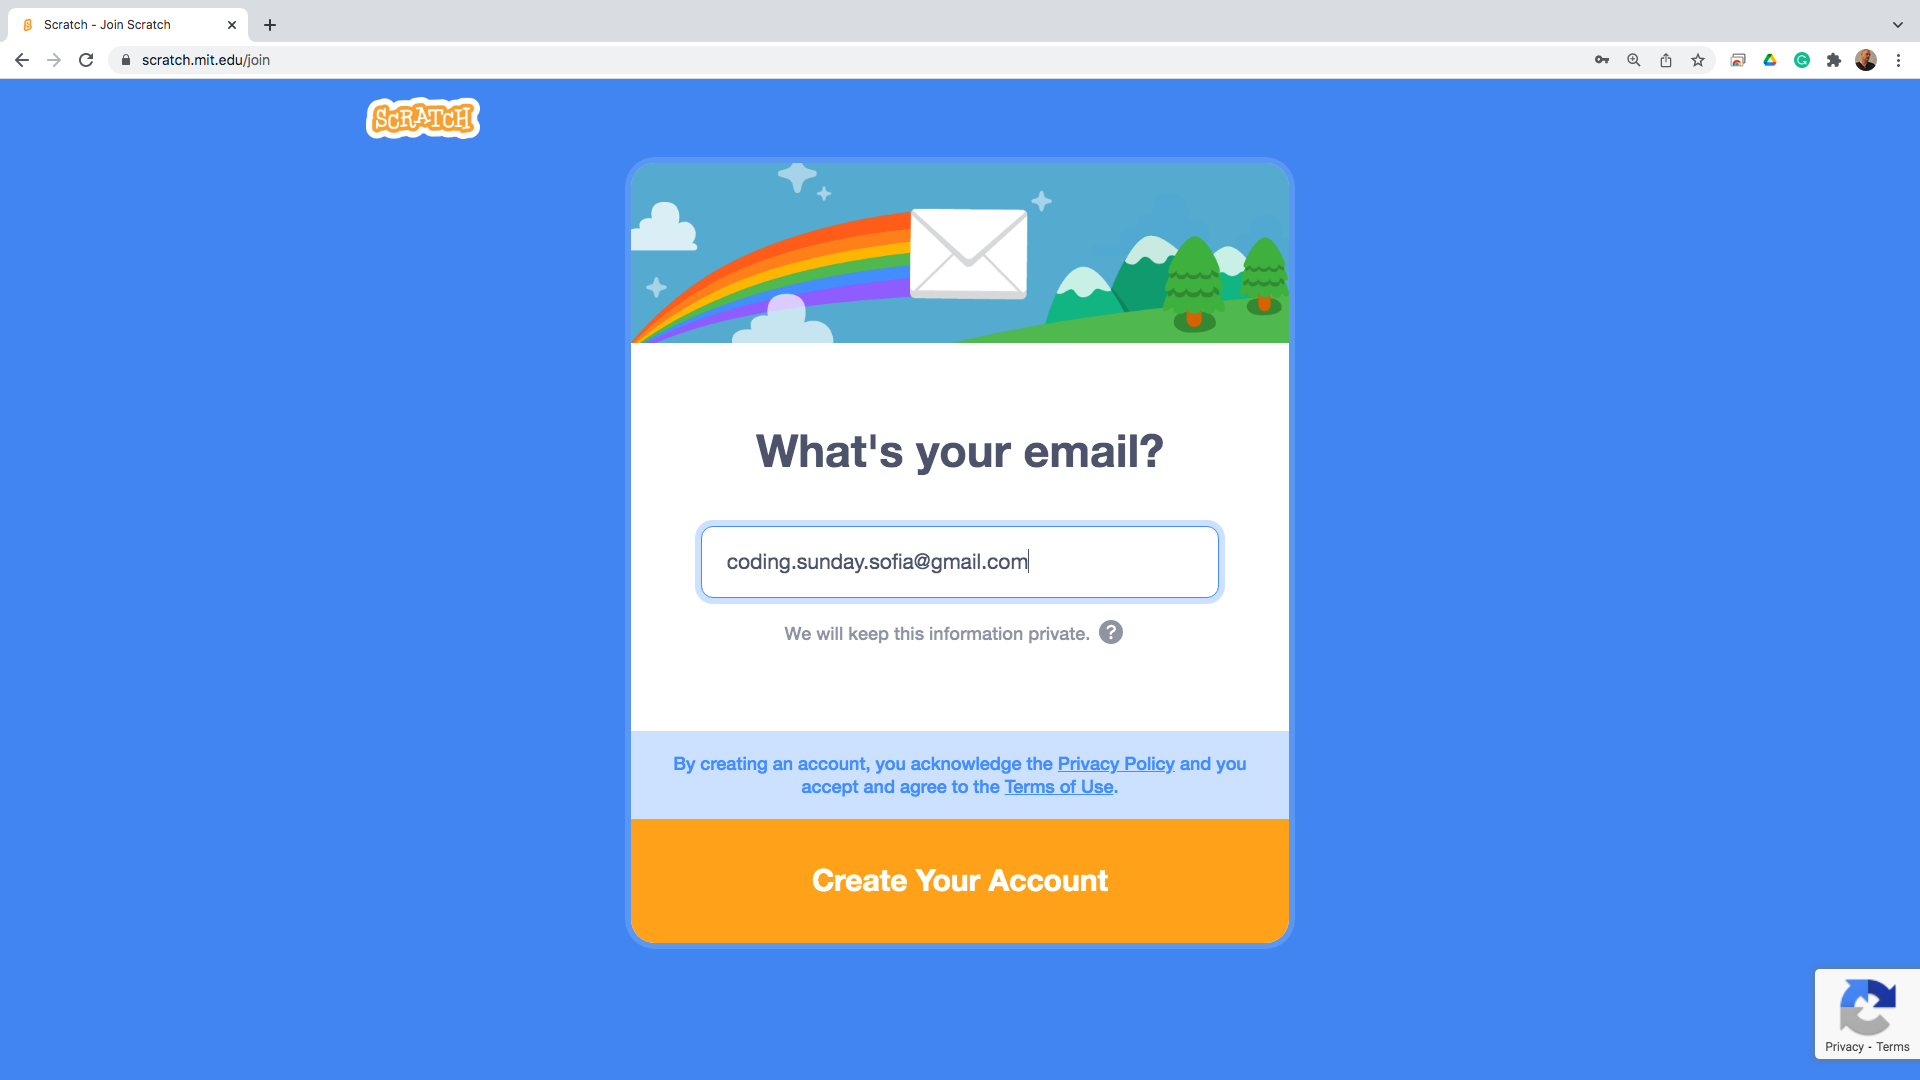
\includegraphics[width=1.0\linewidth,height=0.5\linewidth]{fig010006.png}
   \caption{User email address}
\label{fig010006}
\end{figure}

The system's user registration process is almost complete (Fig. \ref{fig010007}). All that remains is the step to confirm the selected e-mail address.

\begin{figure}[H]
   \centering
   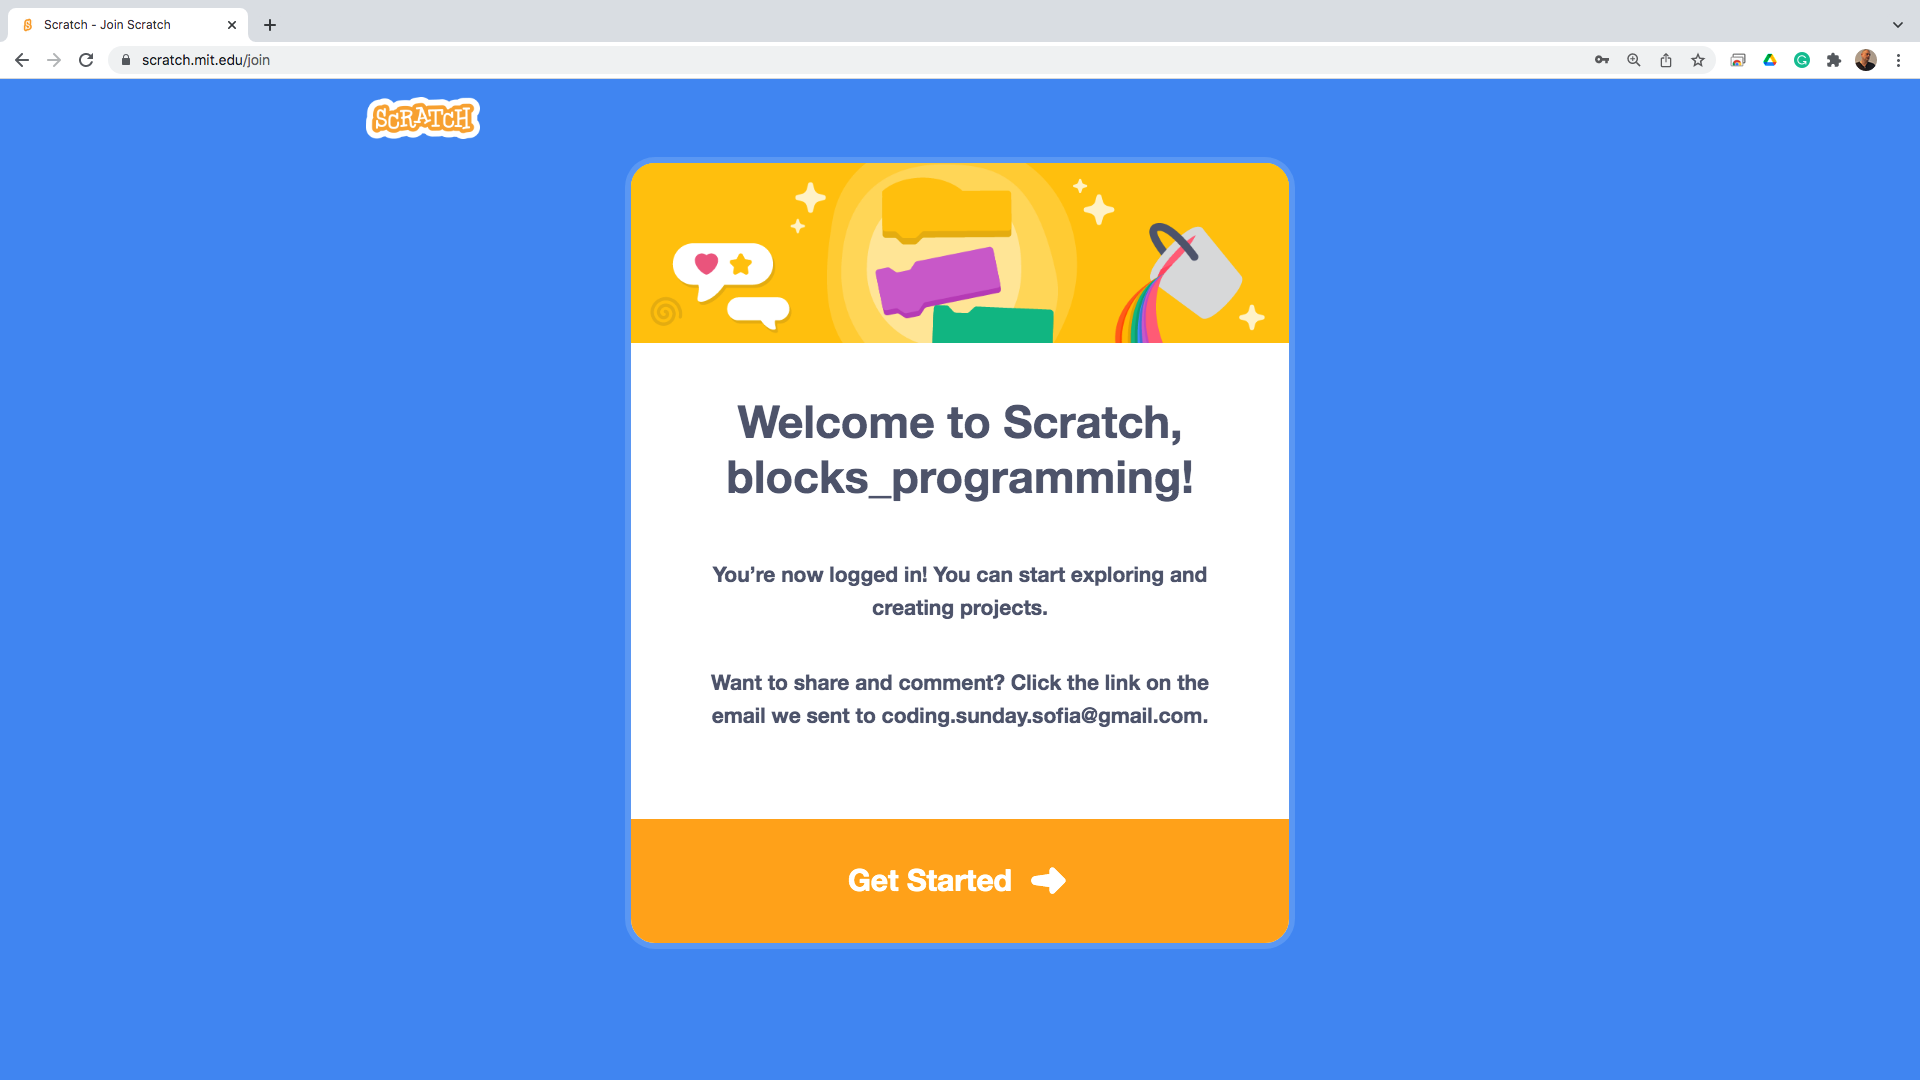
\includegraphics[width=1.0\linewidth,height=0.5\linewidth]{fig010007.png}
   \caption{Completing the user information entry process}
\label{fig010007}
\end{figure}

The email to confirm user registration contains an electronic link to the Scratch website (Fig. \ref{fig010008}). This link must be followed to complete the new user registration process.

\begin{figure}[H]
   \centering
   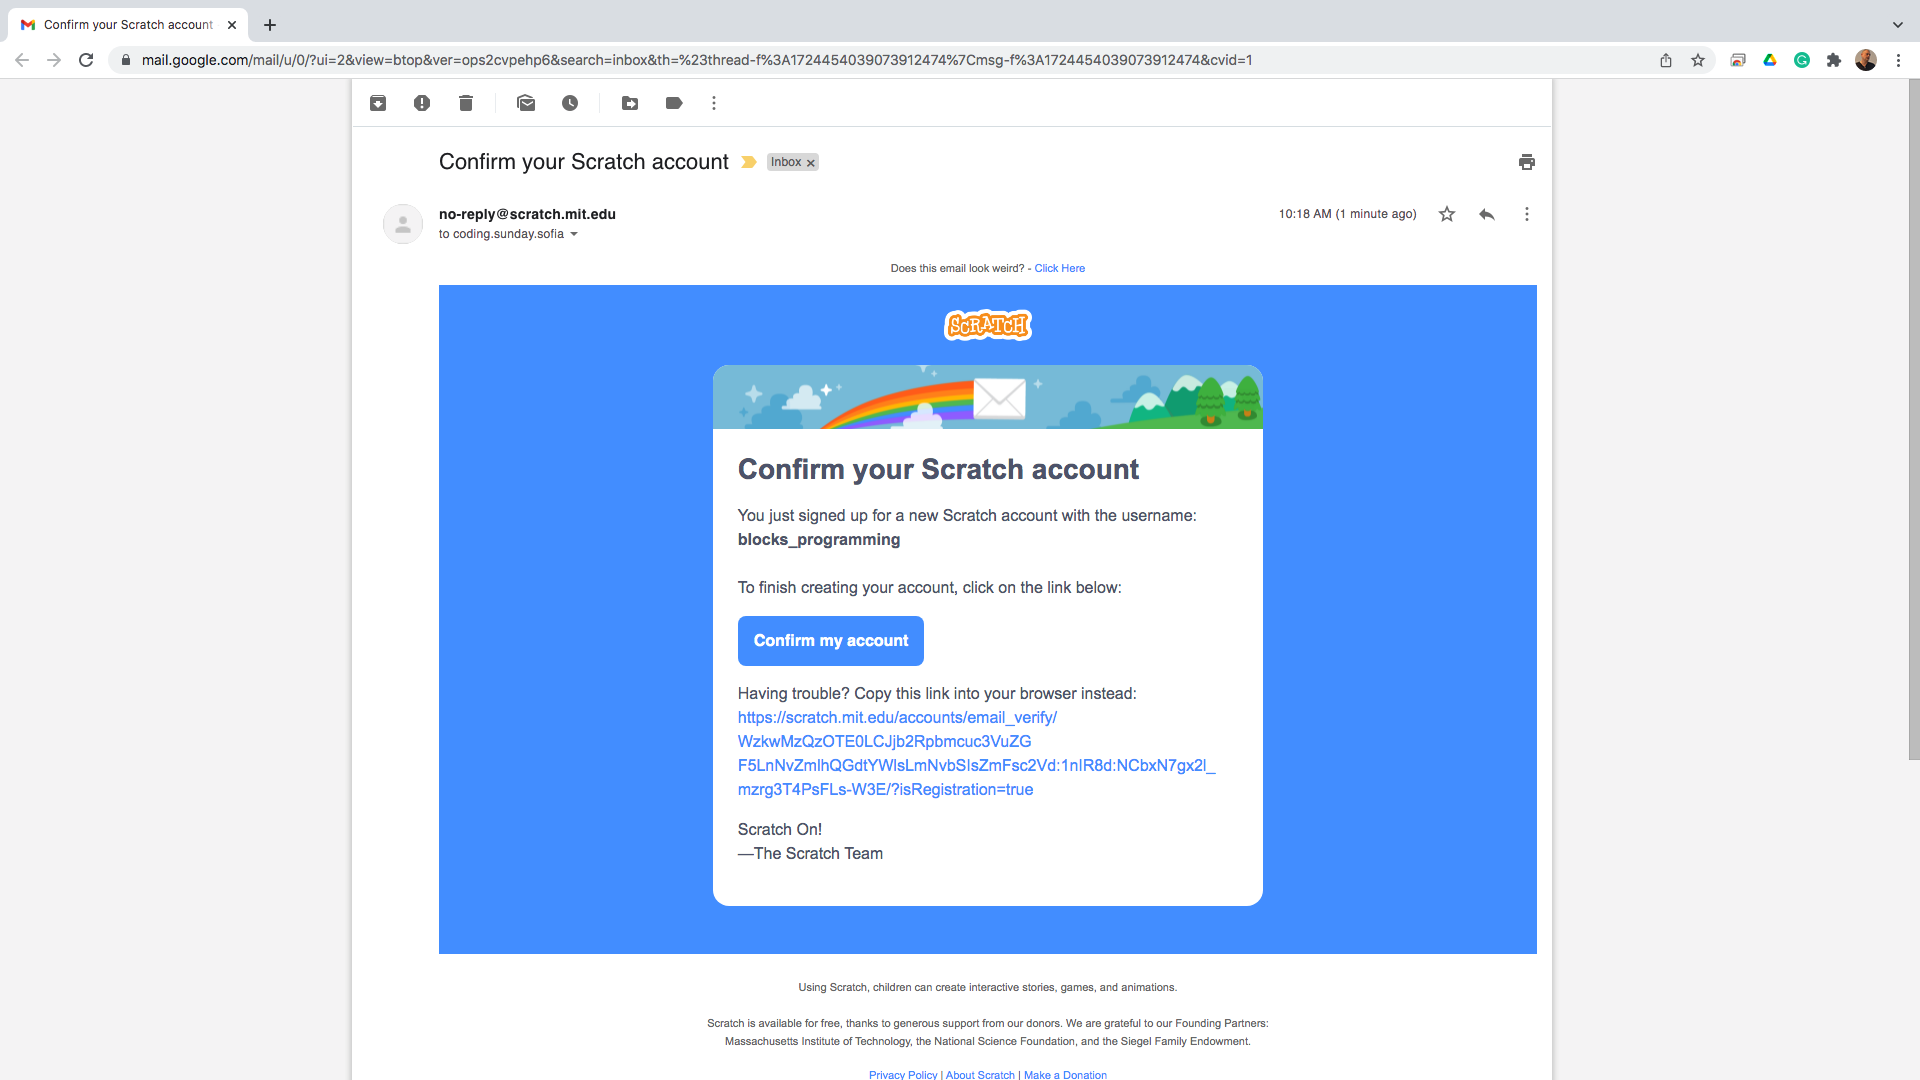
\includegraphics[width=1.0\linewidth,height=0.5\linewidth]{fig010008.png}
   \caption{Email confirmation email}
\label{fig010008}
\end{figure}

The registration of the new user ends with loading the initial working screen (Fig. \ref{fig010009}). At the top right, you can see the username chosen in the first step of the registration process.

\begin{figure}[H]
   \centering
   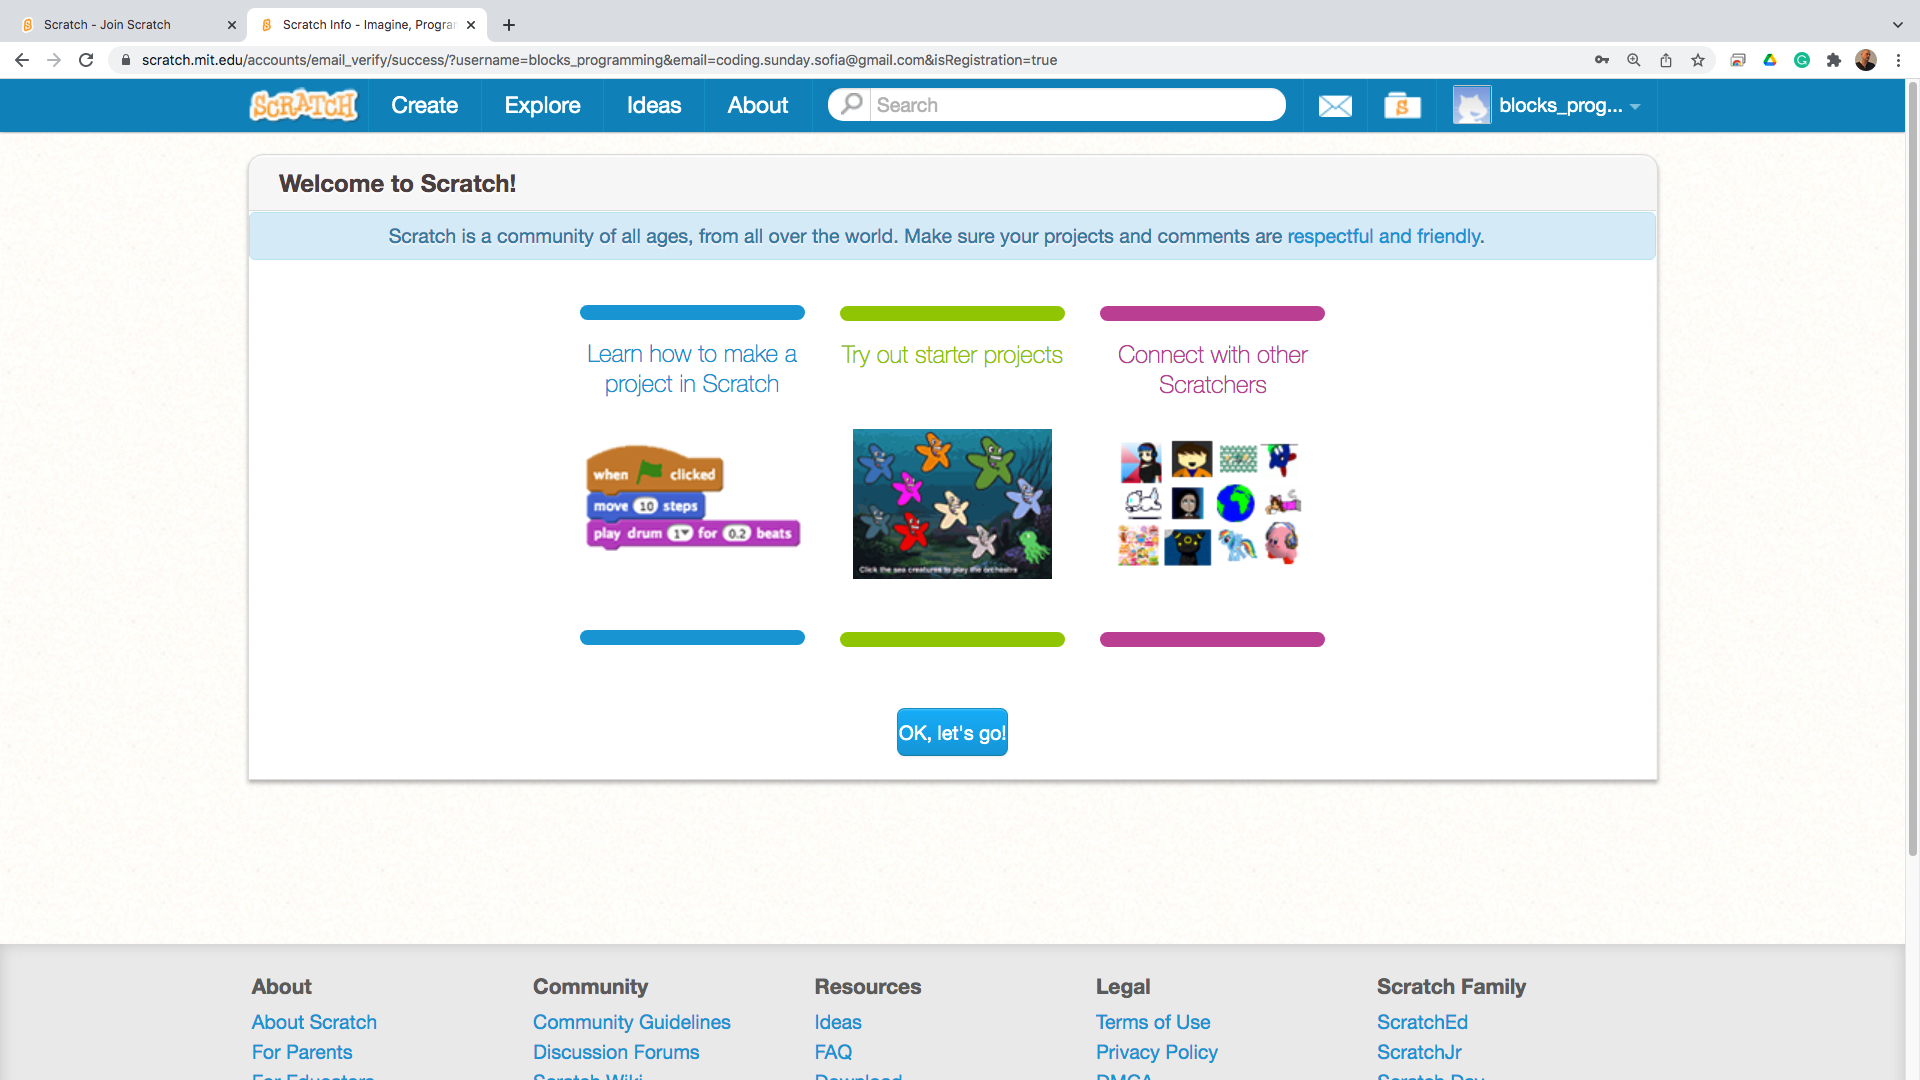
\includegraphics[width=1.0\linewidth,height=0.5\linewidth]{fig010009.png}
   \caption{Home screen}
\label{fig010009}
\end{figure}

Creating a small project demonstrating the development environment can also confirm successful registration. For this purpose, the "Create" option is selected from the menu (Fig. \ref{fig010010}).

\begin{figure}[H]
   \centering
   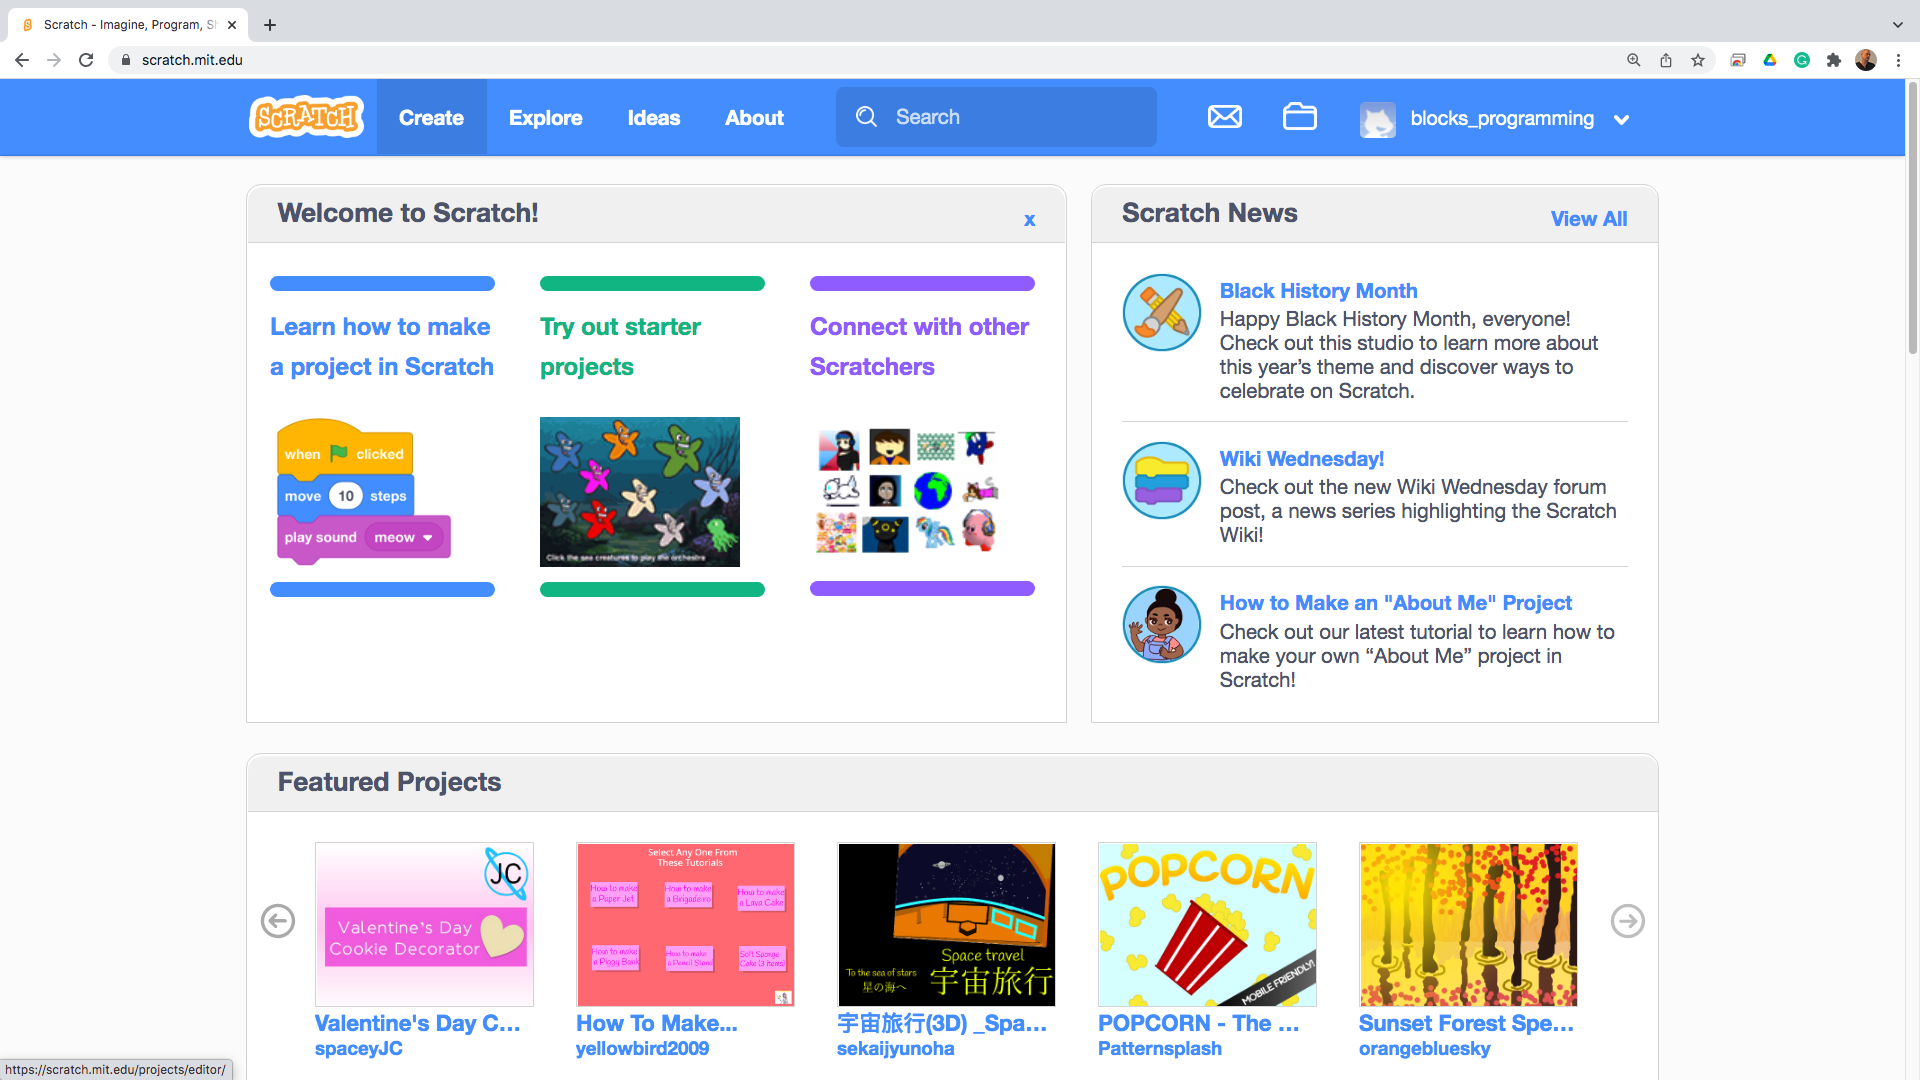
\includegraphics[width=1.0\linewidth,height=0.5\linewidth]{fig010010.png}
   \caption{Selecting a New Project Menu Option}
\label{fig010010}
\end{figure}

Creating a new project goes through a series of steps related to allocating the initially needed resources (Fig. \ref{fig010011}).

\begin{figure}[H]
   \centering
   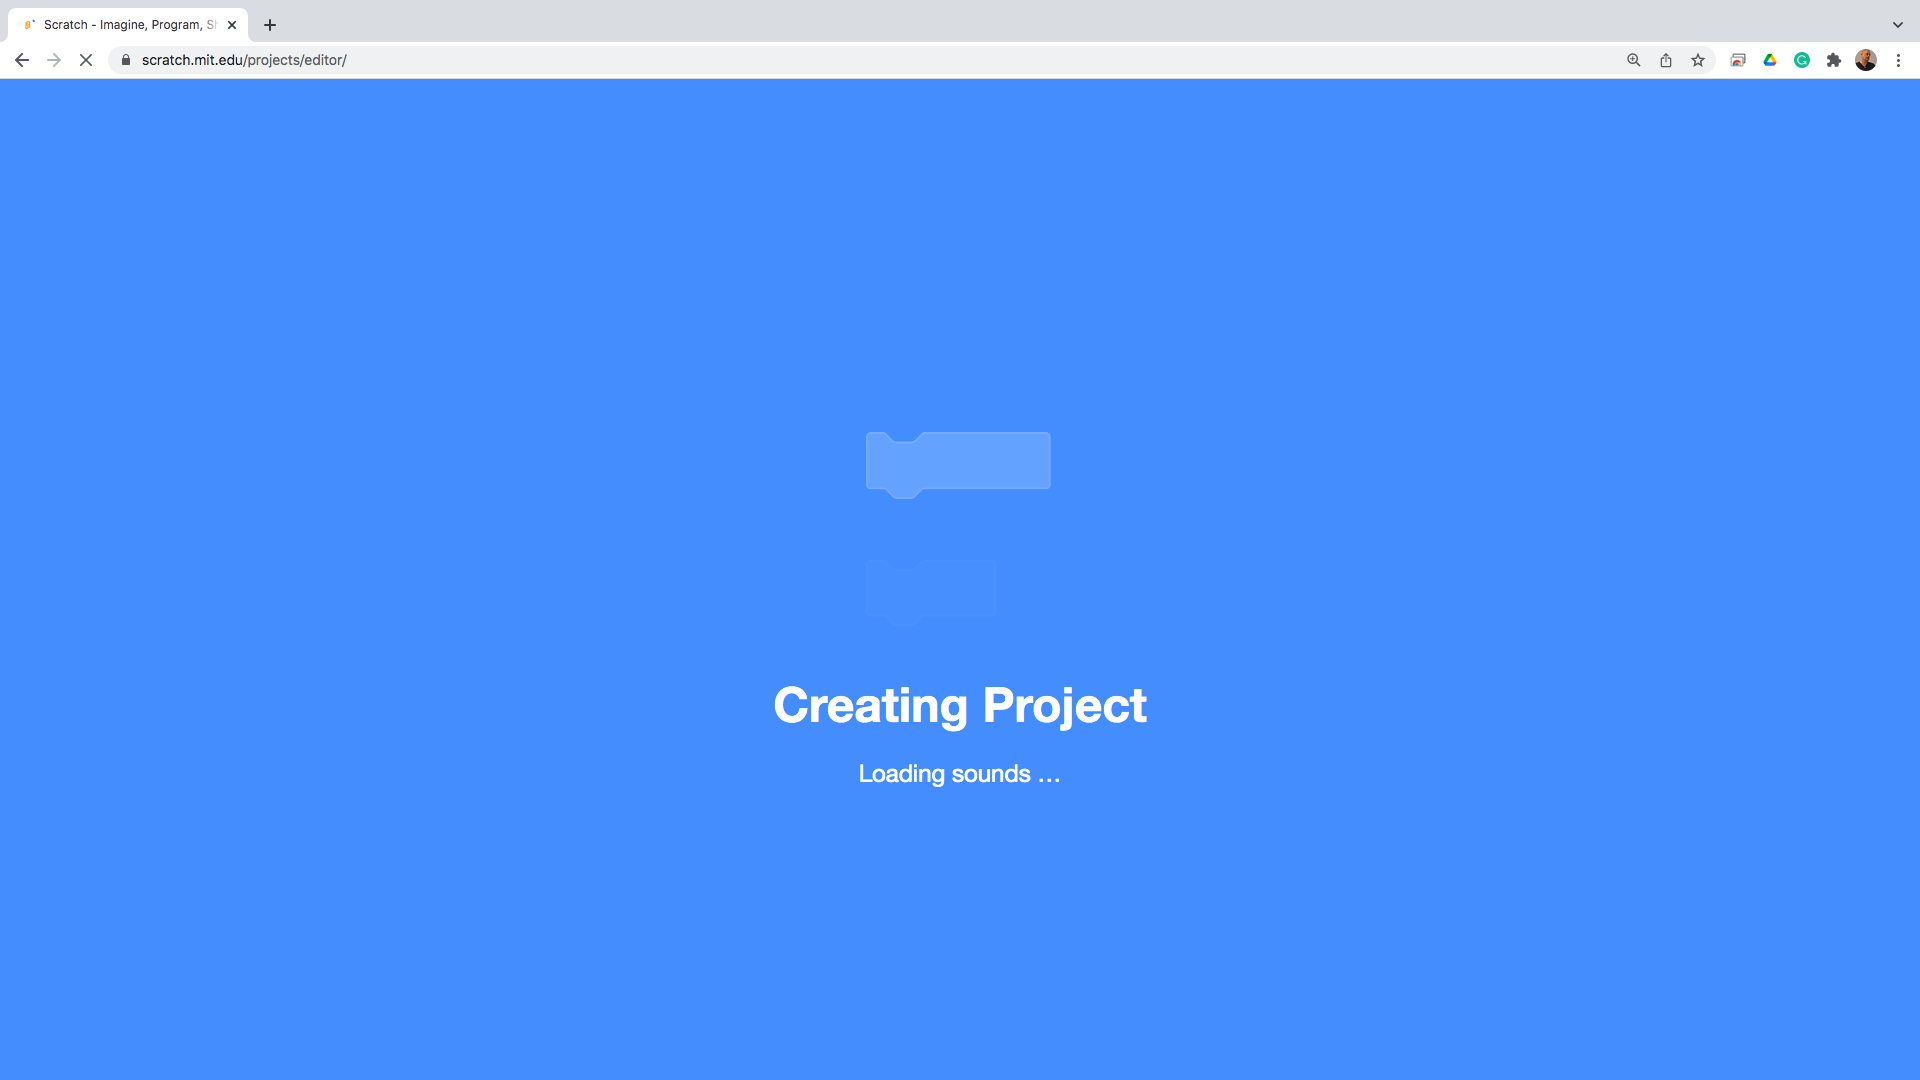
\includegraphics[width=1.0\linewidth,height=0.5\linewidth]{fig010011.png}
   \caption{Loading Resources}
\label{fig010011}
\end{figure}

The workspace is visualized after loading the new project (Fig. \ref{fig010012}). On the far left is the list of possible program instructions in the form of puzzle pieces. In the central part is the workspace where the instructions are arranged. And on the far right is the active stage, where the actions embedded in the instructions are visualized.

\begin{figure}[H]
   \centering
   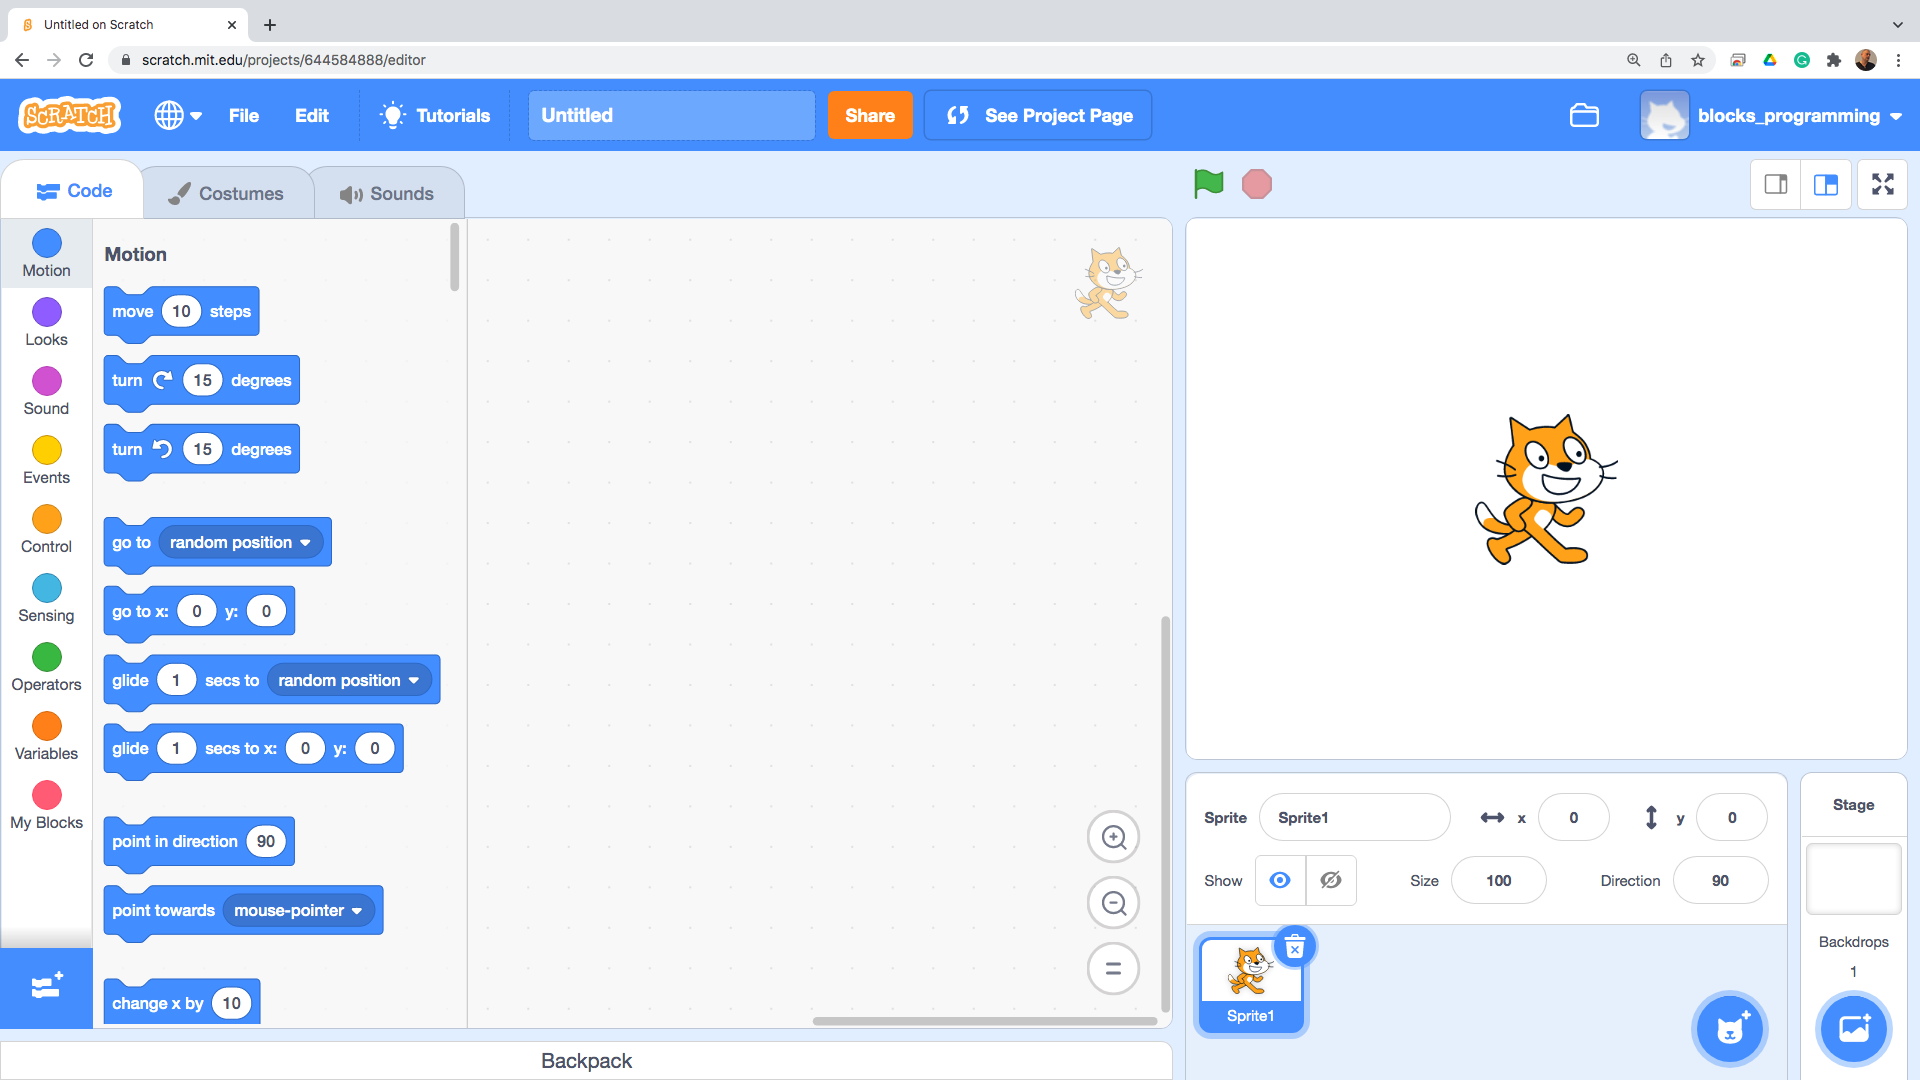
\includegraphics[width=1.0\linewidth,height=0.5\linewidth]{fig010012.png}
   \caption{Workspace Organization}
\label{fig010012}
\end{figure}

Every computer program has its starting point and its ending point. In Scratch, there is a particular block (program instruction) for the beginning of the program, which is shown in Fig. \ref{fig010013}. The execution of the programs written in Scratch starts when the green flag is pressed. Therefore, the program launch block is bound to the green flag click event.

\begin{figure}[H]
   \centering
   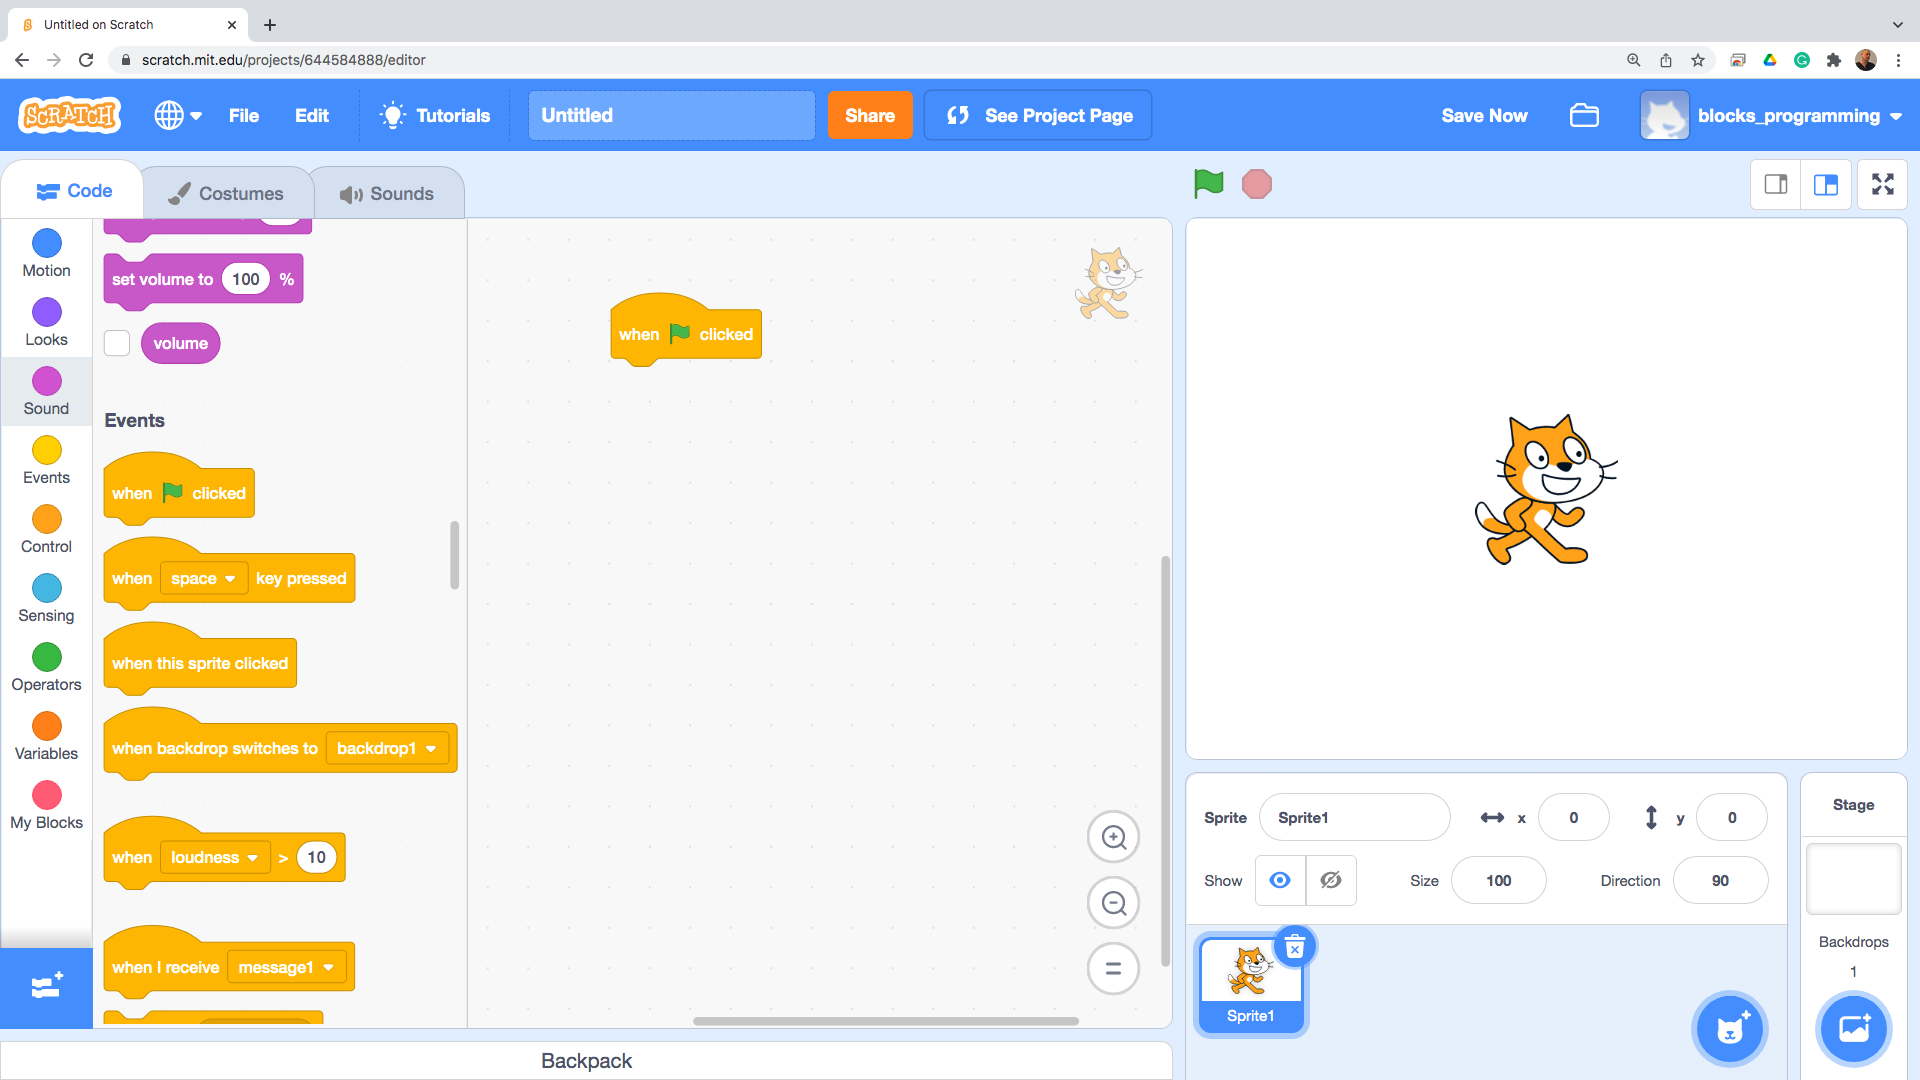
\includegraphics[width=1.0\linewidth,height=0.5\linewidth]{fig010013.png}
   \caption{Start of program}
\label{fig010013}
\end{figure}

One of the most intuitive and, simultaneously, easy-to-understand instructions is to move by a certain number of steps (Fig. \ref{fig010014}). The main actor in the opening scene of Scratch is the orange cat. If the scene is not changed, the instructions to perform various actions are directed directly to that cat.

\begin{figure}[H]
   \centering
   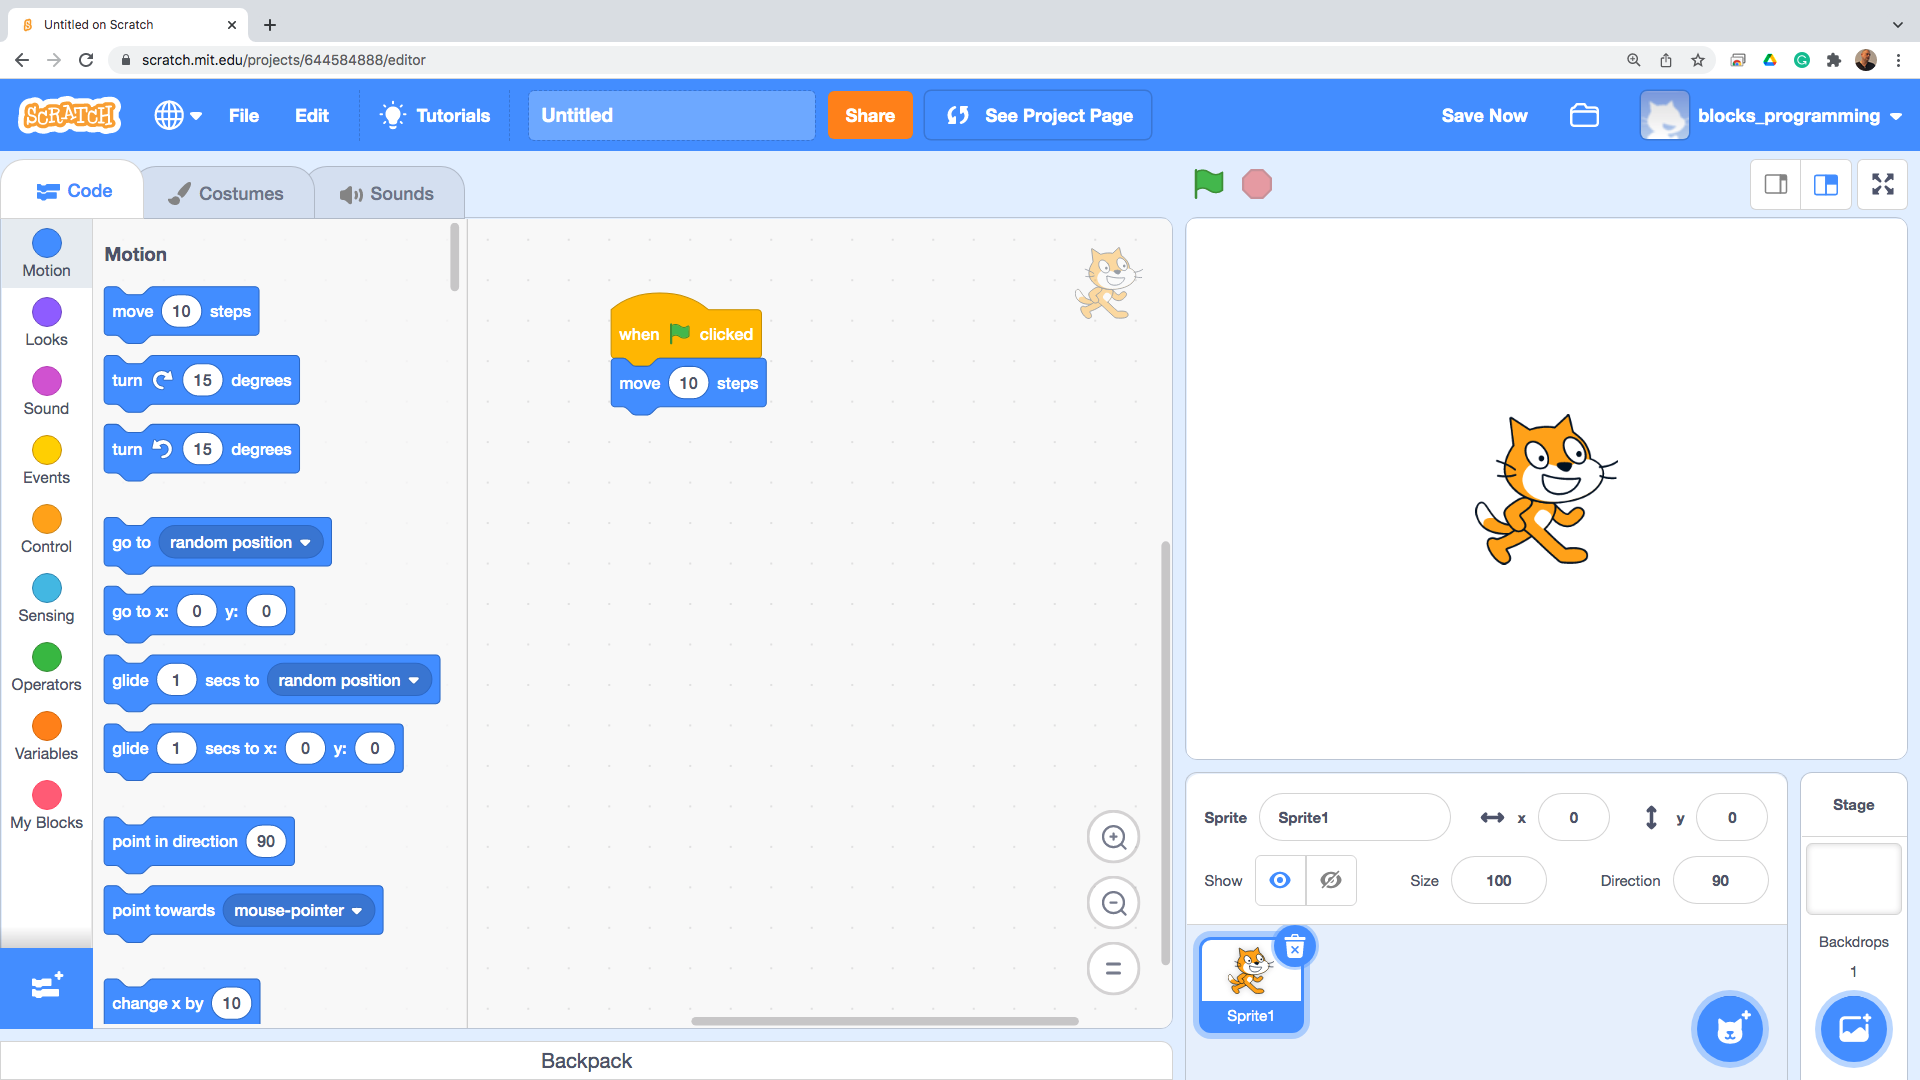
\includegraphics[width=1.0\linewidth,height=0.5\linewidth]{fig010014.png}
   \caption{Step-by-step instructions}
\label{fig010014}
\end{figure}

After the cat is moved, there must be a waiting pause so that the move is visually noted. For this purpose, a wait instruction can be implemented for a certain number of seconds (Fig. \ref{fig010015}).

\begin{figure}[H]
   \centering
   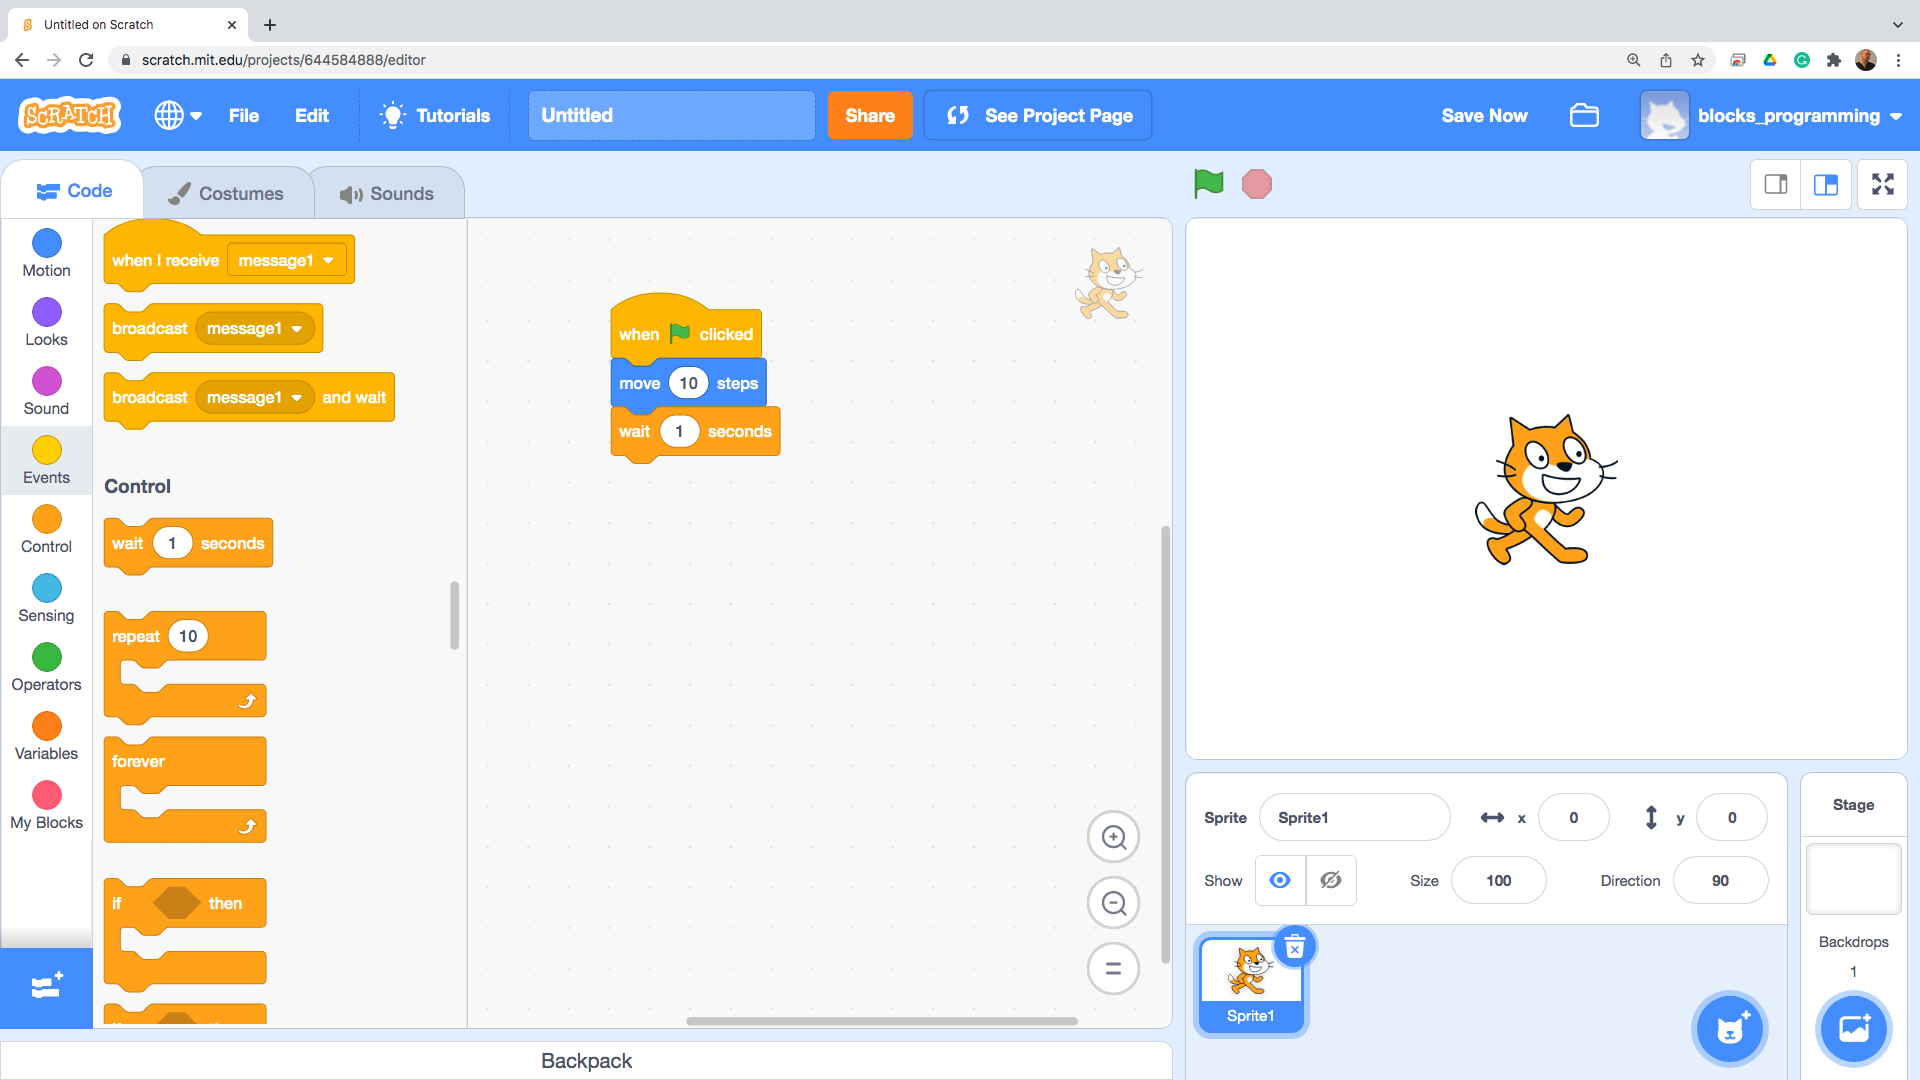
\includegraphics[width=1.0\linewidth,height=0.5\linewidth]{fig010015.png}
   \caption{Wait instruction}
\label{fig010015}
\end{figure}

After the wait, the cat can return to its original position by executing a move instruction with a negative number of steps (Fig. \ref{fig010016}).

\begin{figure}[H]
   \centering
   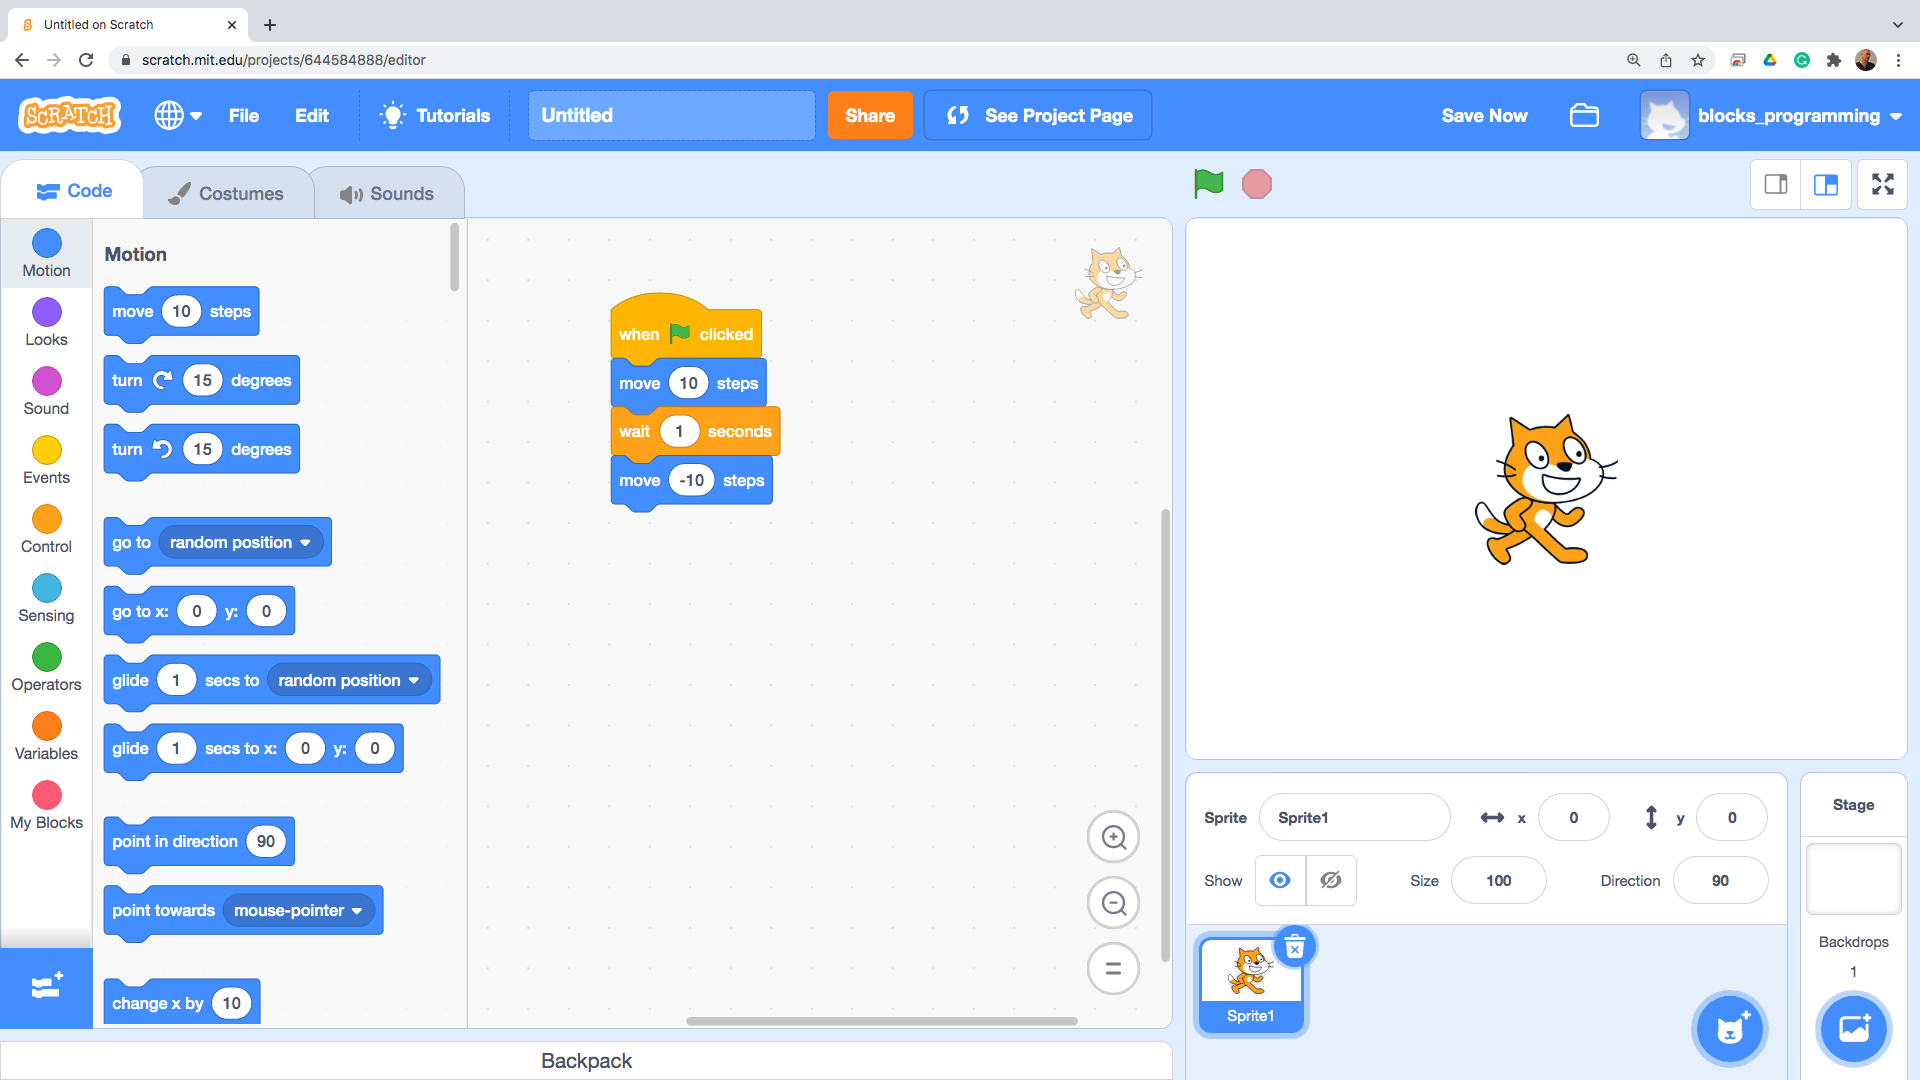
\includegraphics[width=1.0\linewidth,height=0.5\linewidth]{fig010016.png}
   \caption{Instructions for moving back}
\label{fig010016}
\end{figure}

After all the intended instructions have been executed, it is reasonable to end the program, for which a separate block is provided in the list of instructions (Fig. \ref{fig010017}).

\begin{figure}[H]
   \centering
   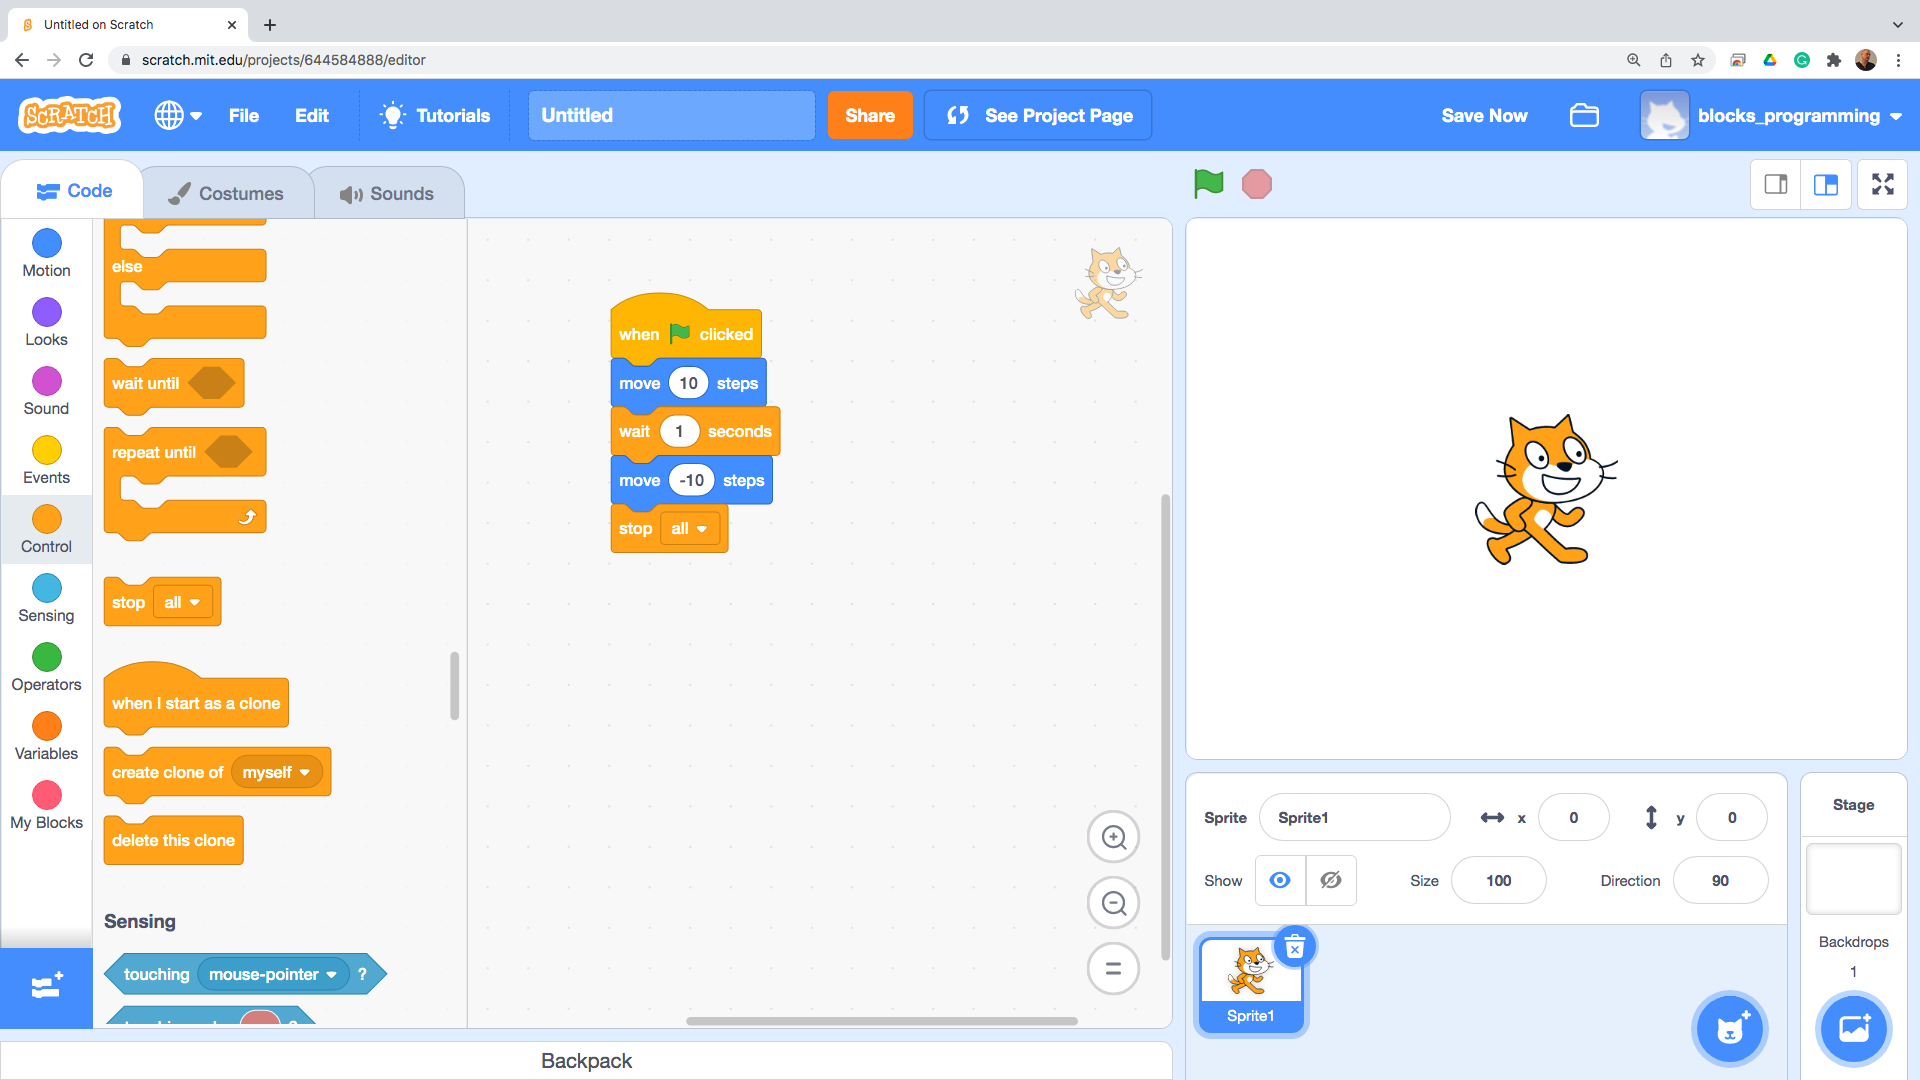
\includegraphics[width=1.0\linewidth,height=0.5\linewidth]{fig010017.png}
   \caption{End instruction}
\label{fig010017}
\end{figure}

The program written in this way is executed by pressing the green flag (Fig. \ref{fig010018}), and if an emergency stop is needed, press the red circle to the right of the green flag.

\begin{figure}[H]
   \centering
   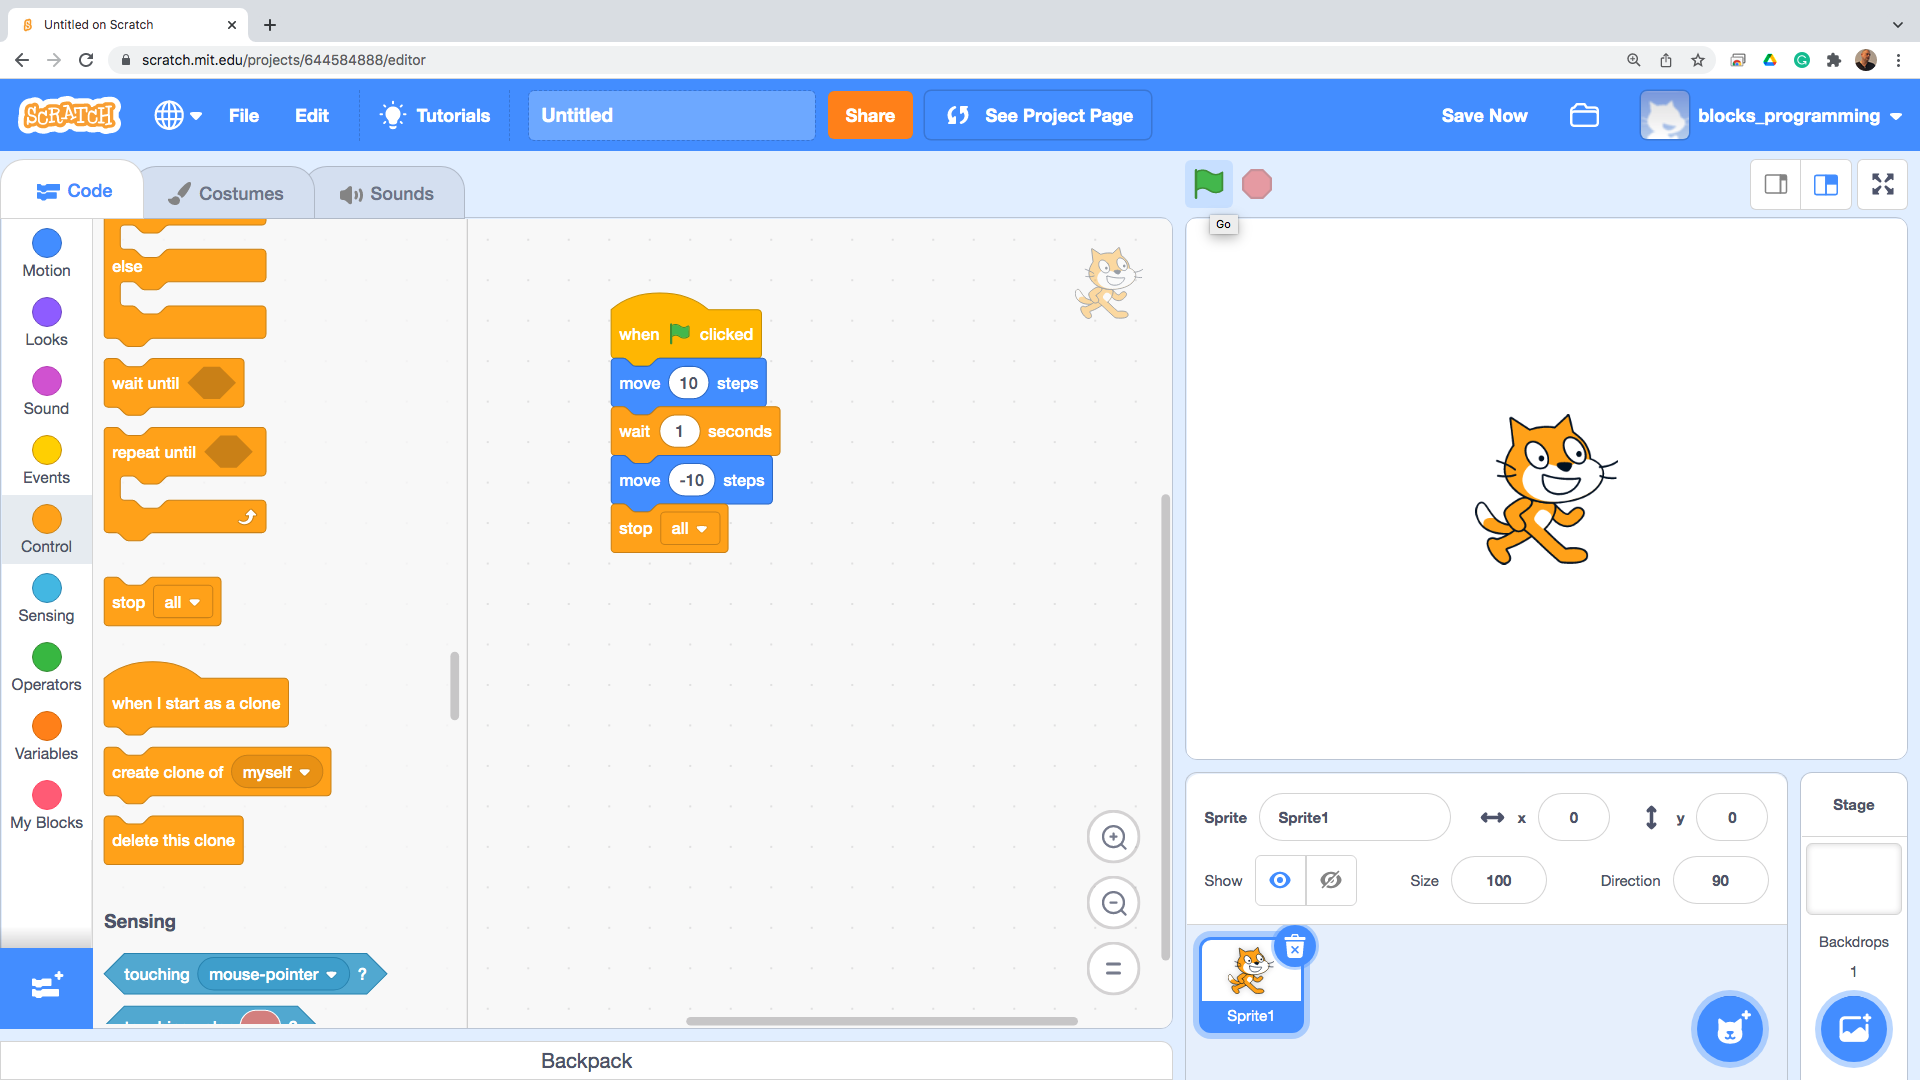
\includegraphics[width=1.0\linewidth,height=0.5\linewidth]{fig010018.png}
   \caption{Program Execution}
\label{fig010018}
\end{figure}

Each program that is written in Scratch is placed in a separate project. All of the user's projects can be accessed from the "My Stuff" menu, which is part of the list of options for handling the registered user (Fig. \ref{fig010019}).

\begin{figure}[H]
   \centering
   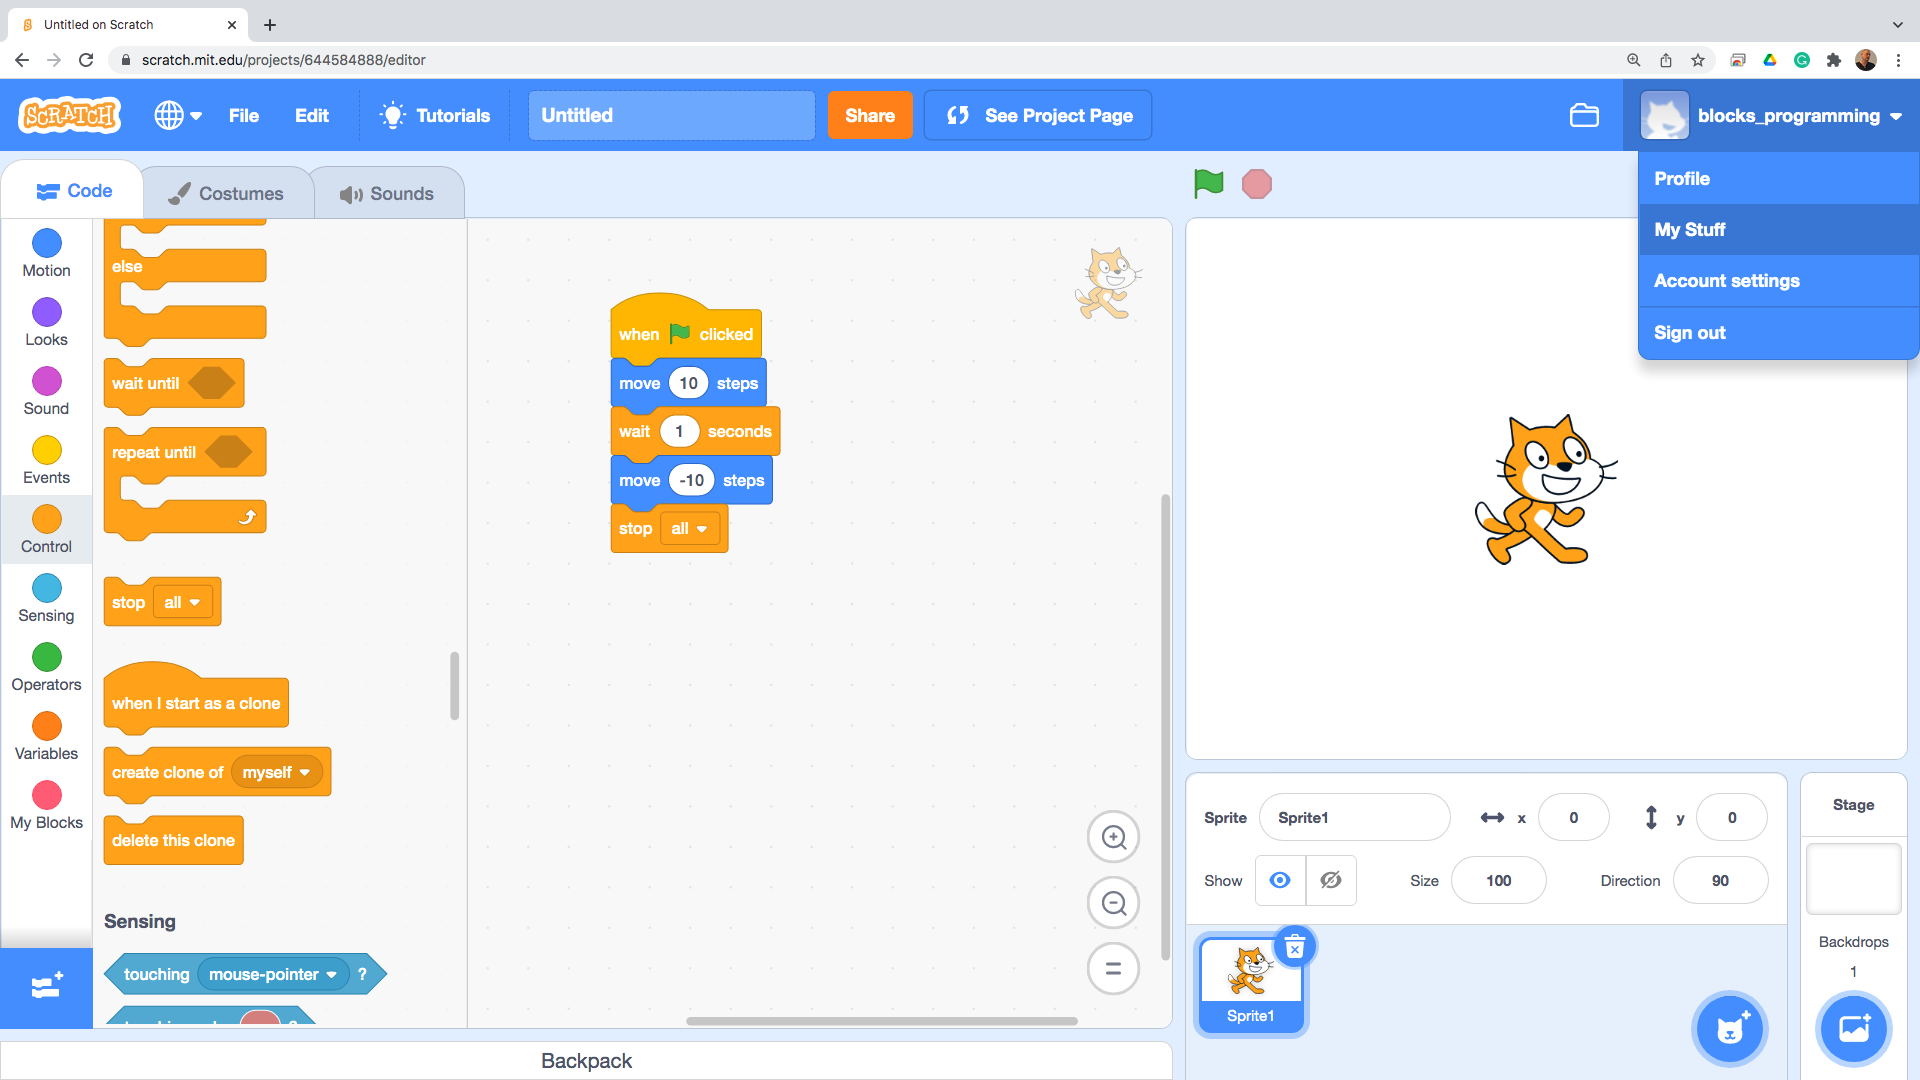
\includegraphics[width=1.0\linewidth,height=0.5\linewidth]{fig010019.png}
   \caption{Project Organization Menu}
\label{fig010019}
\end{figure}

Initially, each project has a working name (Fig. \ref{fig010020}), which can be changed later. One of the most attractive advantages of the programming environment is that users' projects can be shared (Sharing) with a vast audience. This allows a quick transfer of knowledge and skills and an assessment of the work done.

\begin{figure}[H]
   \centering
   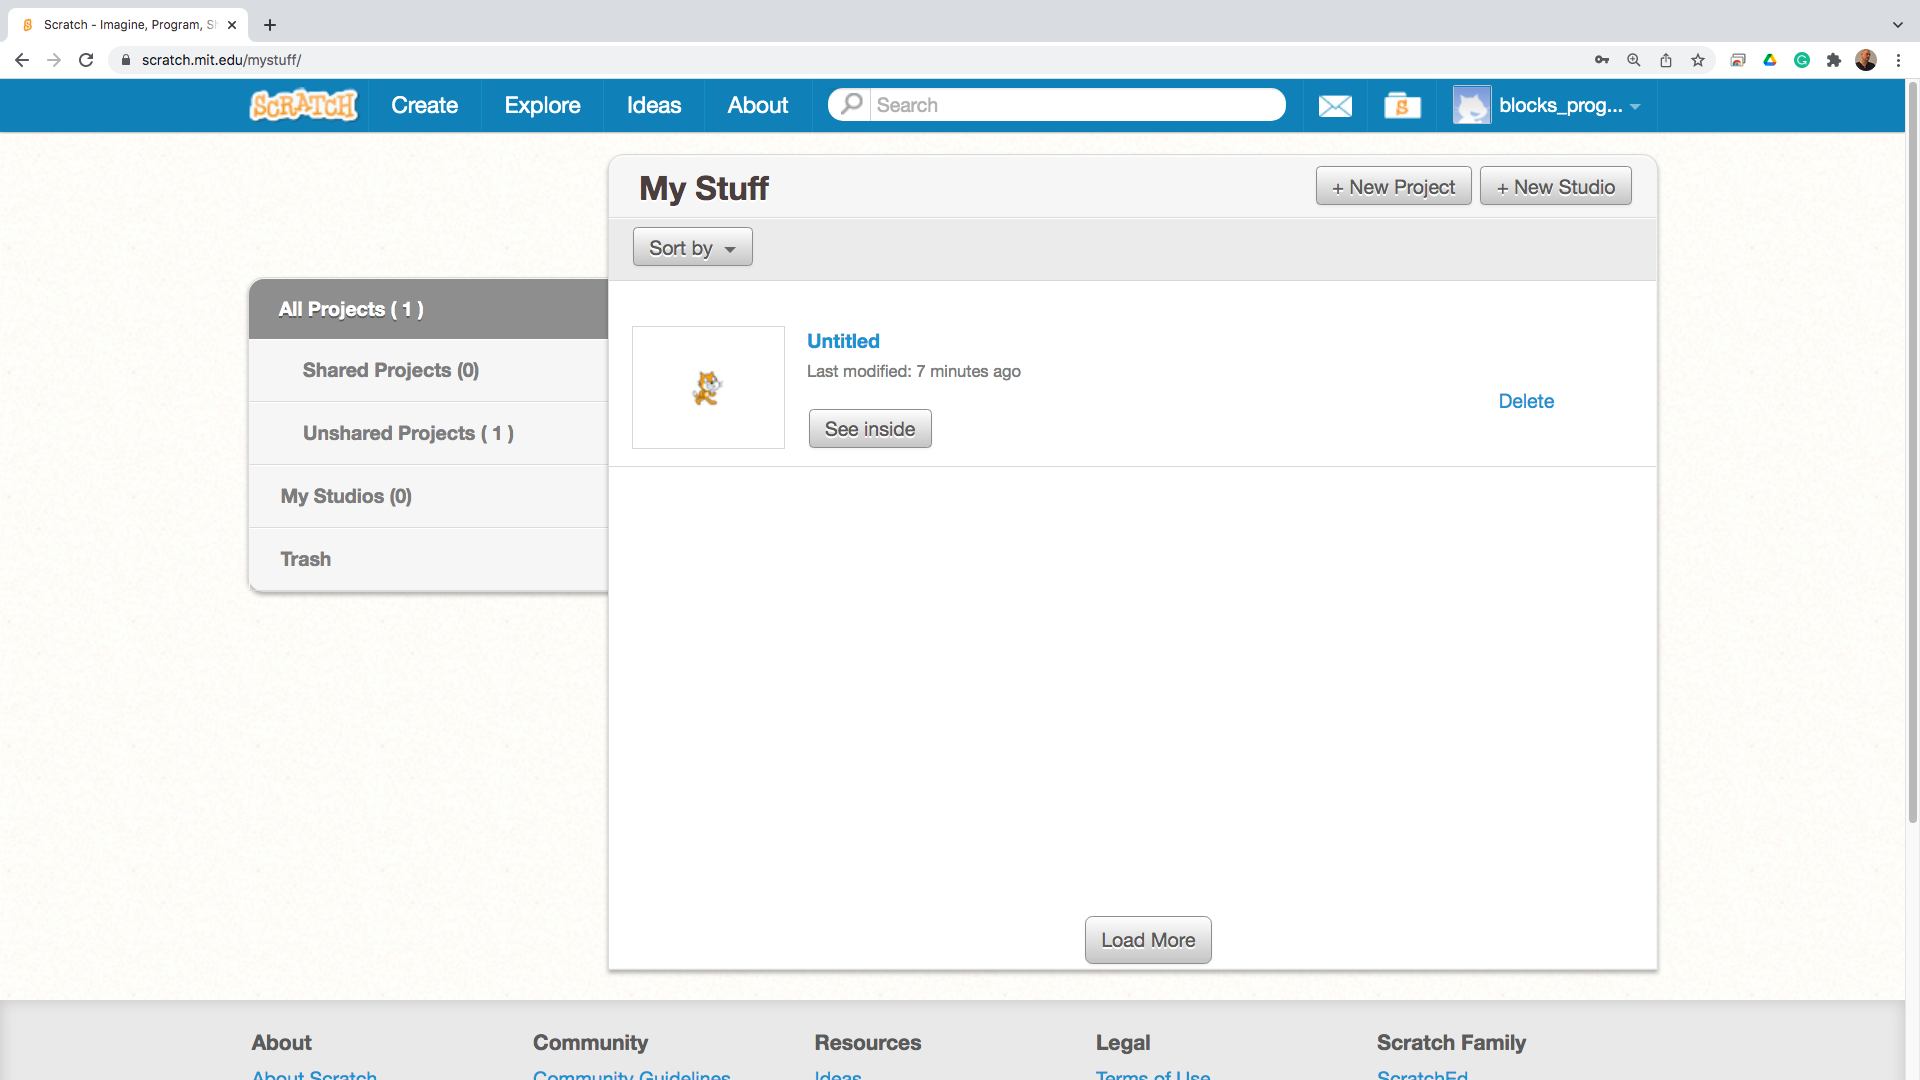
\includegraphics[width=1.0\linewidth,height=0.5\linewidth]{fig010020.png}
   \caption{List of projects}
\label{fig010020}
\end{figure}

The greatest fascination with block languages comes from writing the instructions and forming a complete program, like putting together a puzzle. Almost all children like to put together puzzles. They like bright colors and beautiful pictures. When the charm of classic puzzles is transferred to a field as attractive as programming, the results can be astounding.

\section{Getting Started in App Inventor}

Working in the App Inventor environment begins by loading the main web page (Fig. \ref{fig010021}), which is located at: \\ \href{https://appinventor.mit.edu/}{https:// appinventor.mit.edu/}

\begin{figure}[H]
   \centering
   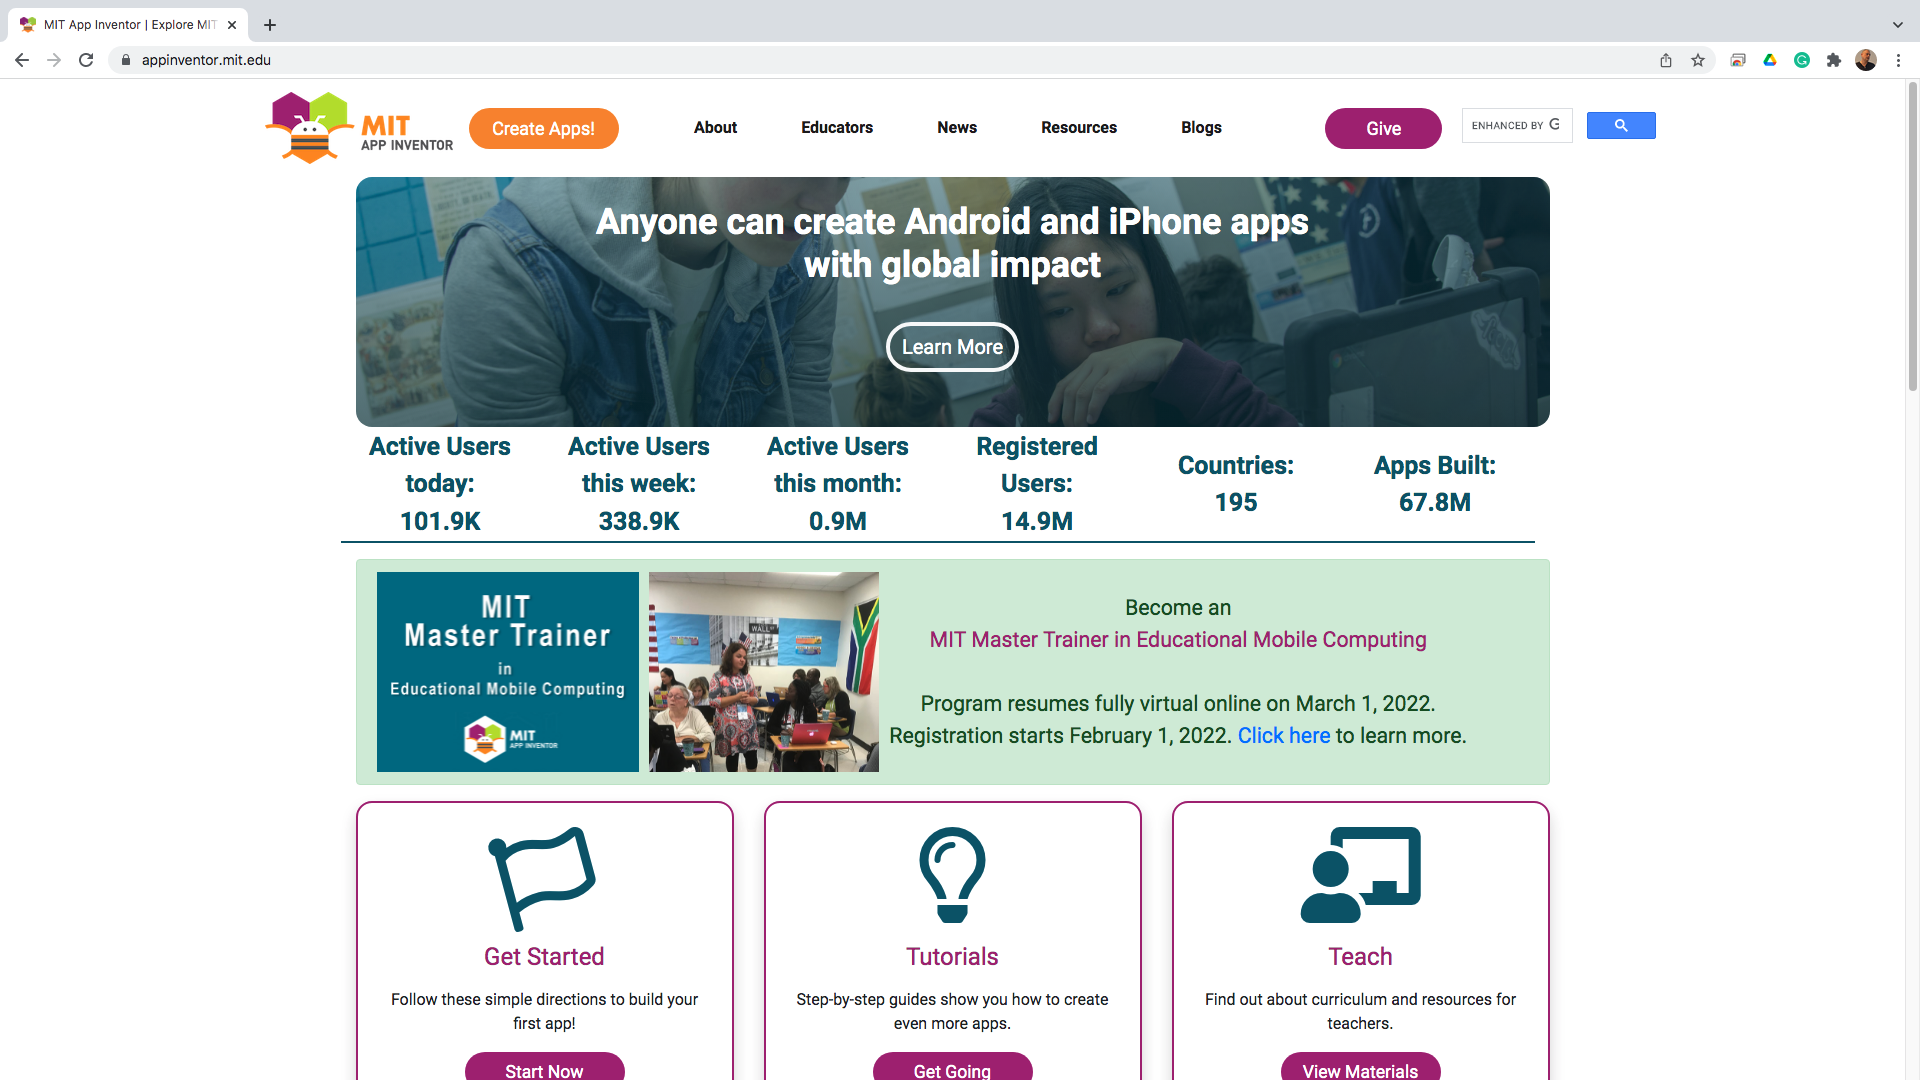
\includegraphics[width=1.0\linewidth,height=0.5\linewidth]{fig010021.png}
   \caption{App Inventor Home Web Page}
\label{fig010021}
\end{figure}

Although App Inventor is also a product of the Massachusetts Institute of Technology, working with it in some aspects differs from how you work in Scratch. App Inventor is also available as a cloud service where registration is required. Unlike Scratch, in App Inventor, you can skip creating a user profile and log in to the system through classic registration in the GMail service. This process starts after selecting the orange "Create Apps!" button (Fig. \ref{fig010022}).

\begin{figure}[H]
   \centering
   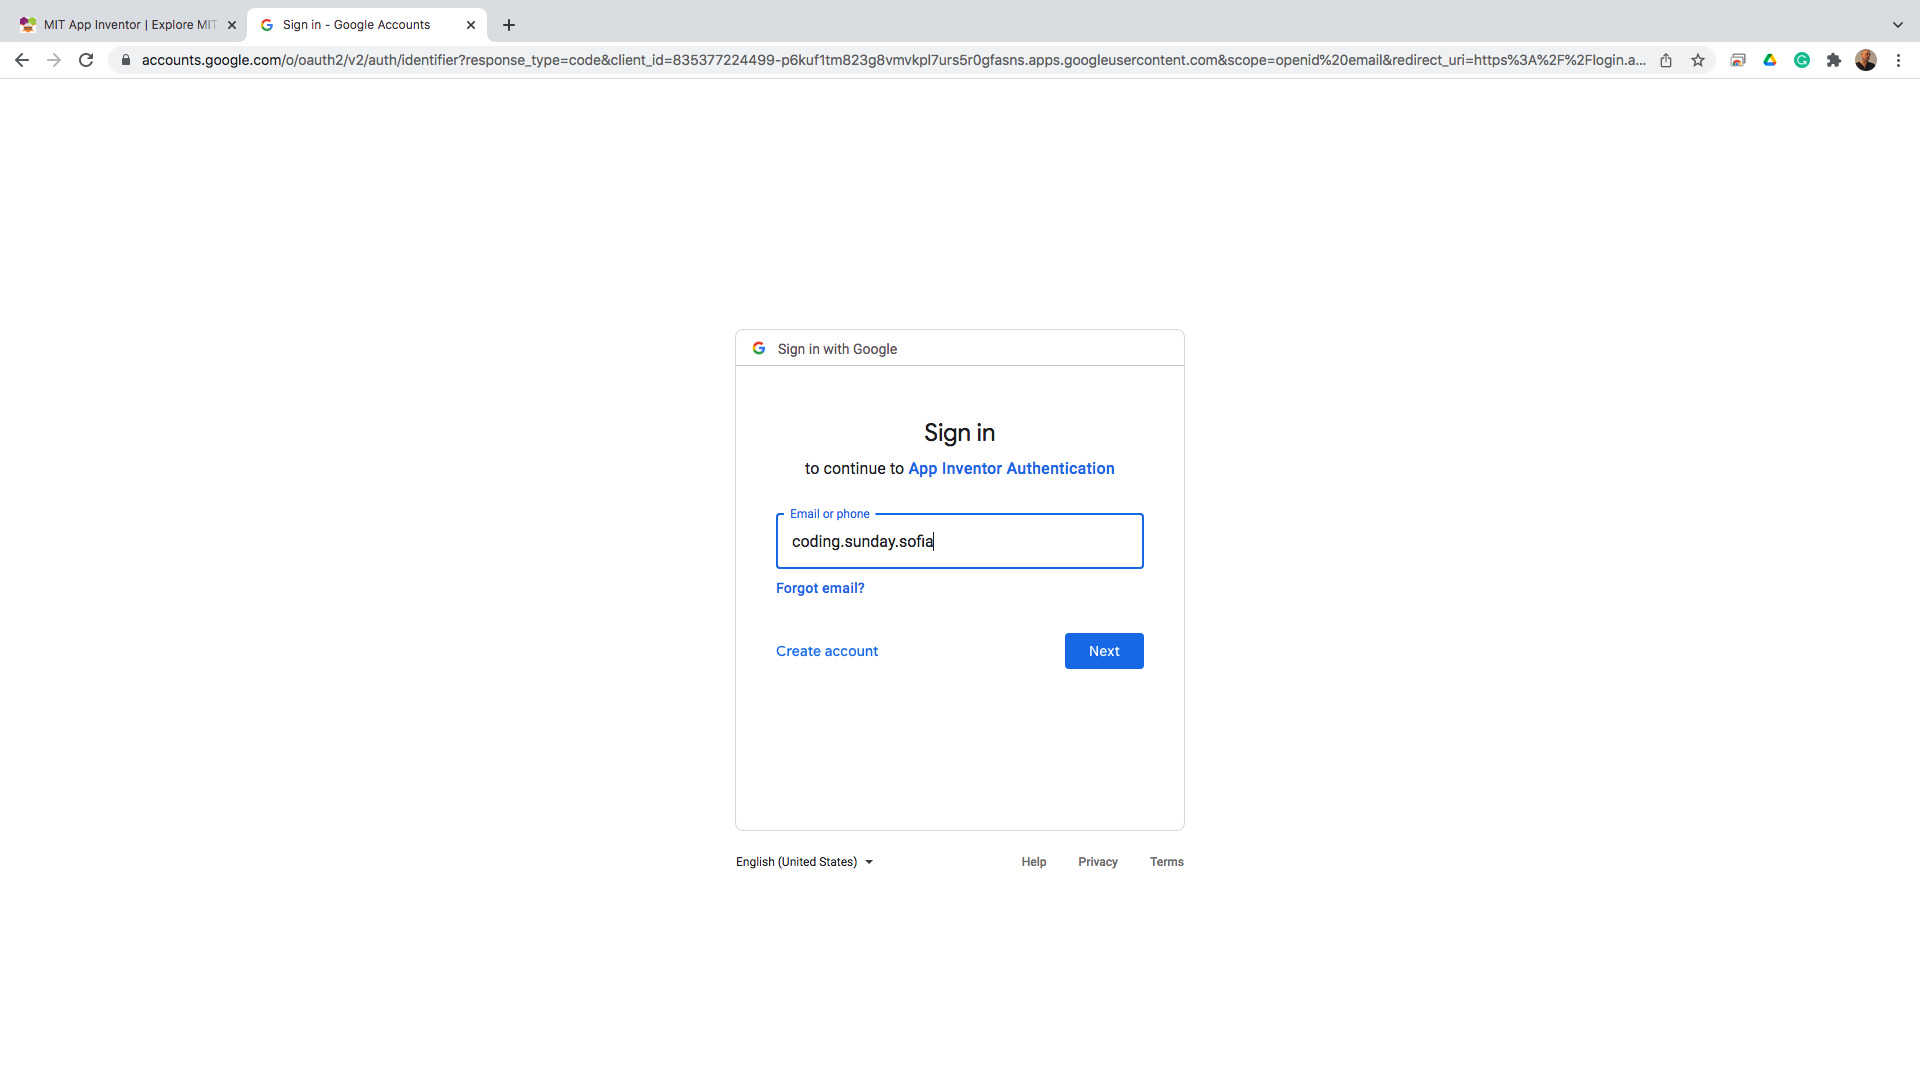
\includegraphics[width=1.0\linewidth,height=0.5\linewidth]{fig010022.png}
   \caption{Choosing a GMail user to log in}
\label{fig010022}
\end{figure}

After selecting a user to work within the App Inventor environment, this user must be authenticated by entering a password (Fig. \ref{fig010023}).

\begin{figure}[H]
   \centering
   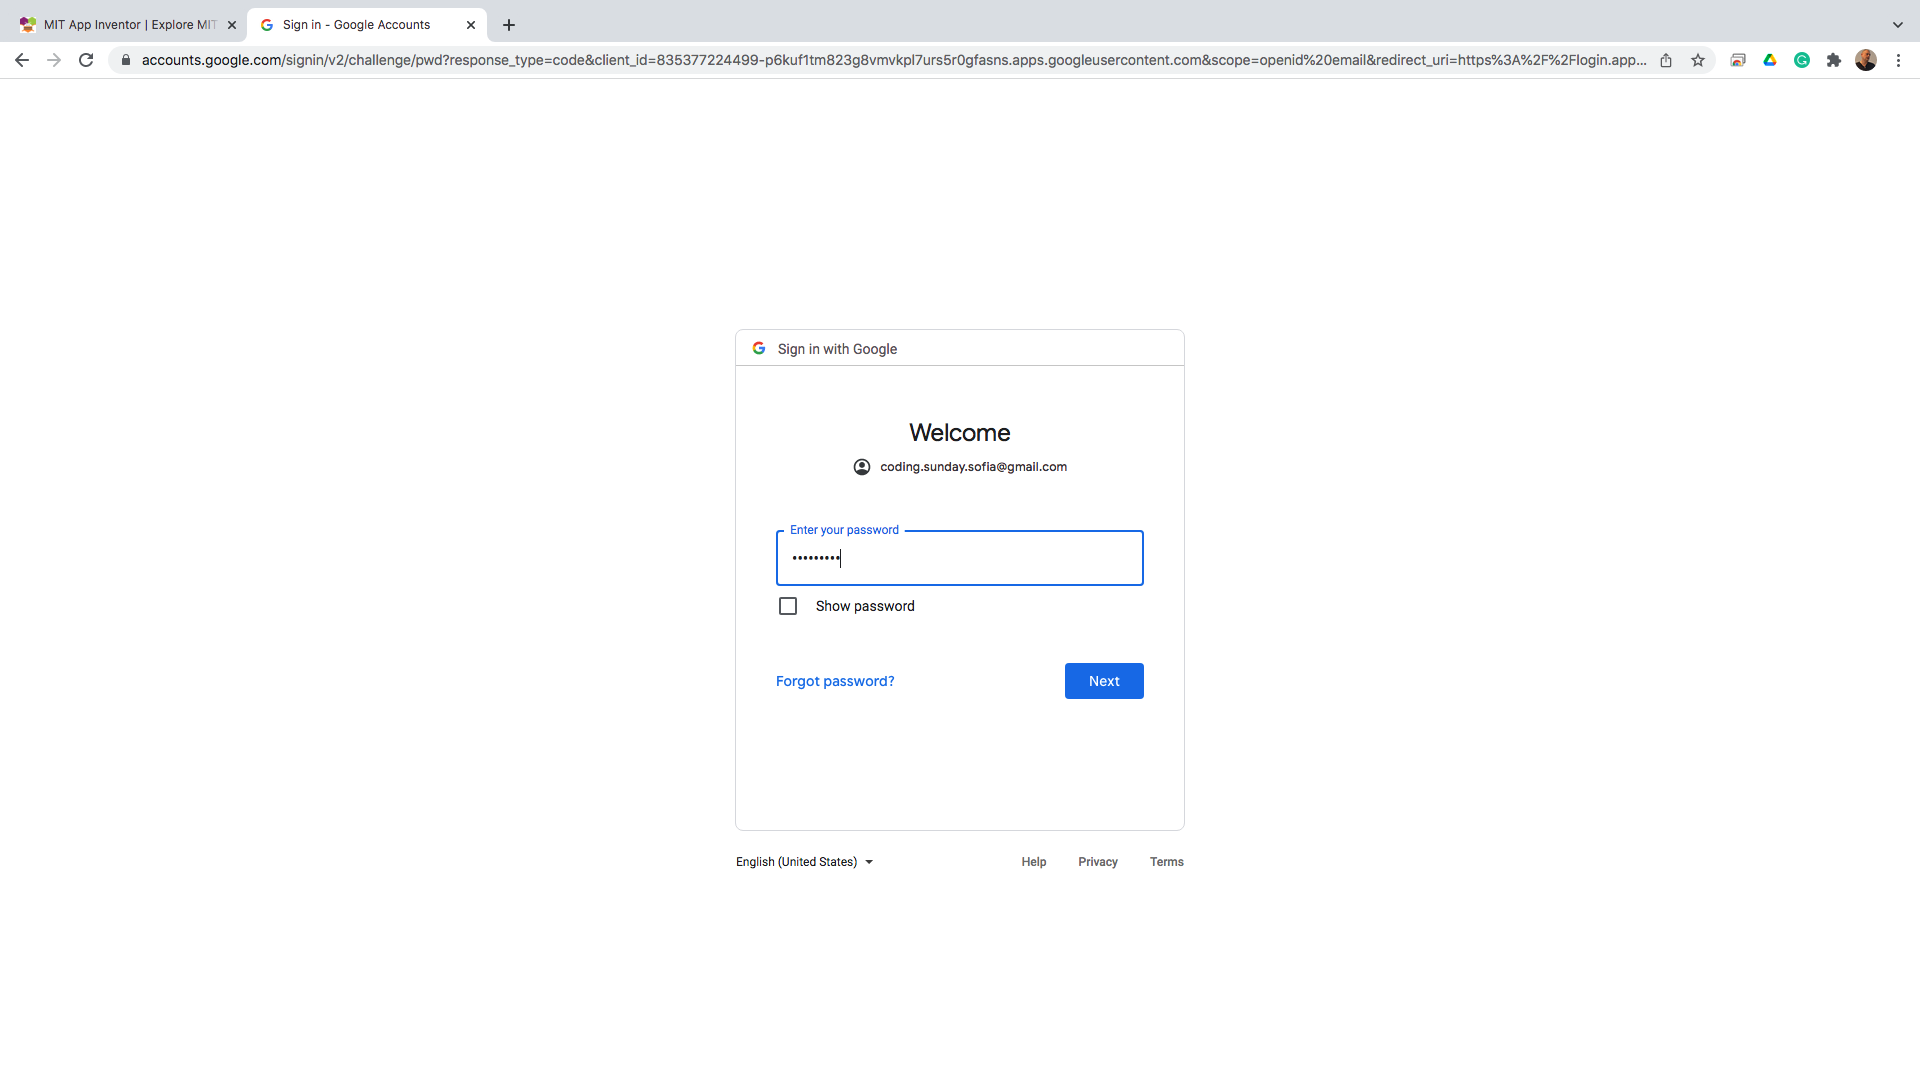
\includegraphics[width=1.0\linewidth,height=0.5\linewidth]{fig010023.png}
   \caption{User Authentication}
\label{fig010023}
\end{figure}

To be allowed to work in the App Inventor programming environment, the user's agreement with the general terms of the platform is required (Fig. \ref{fig010024}).

\begin{figure}[H]
   \centering
   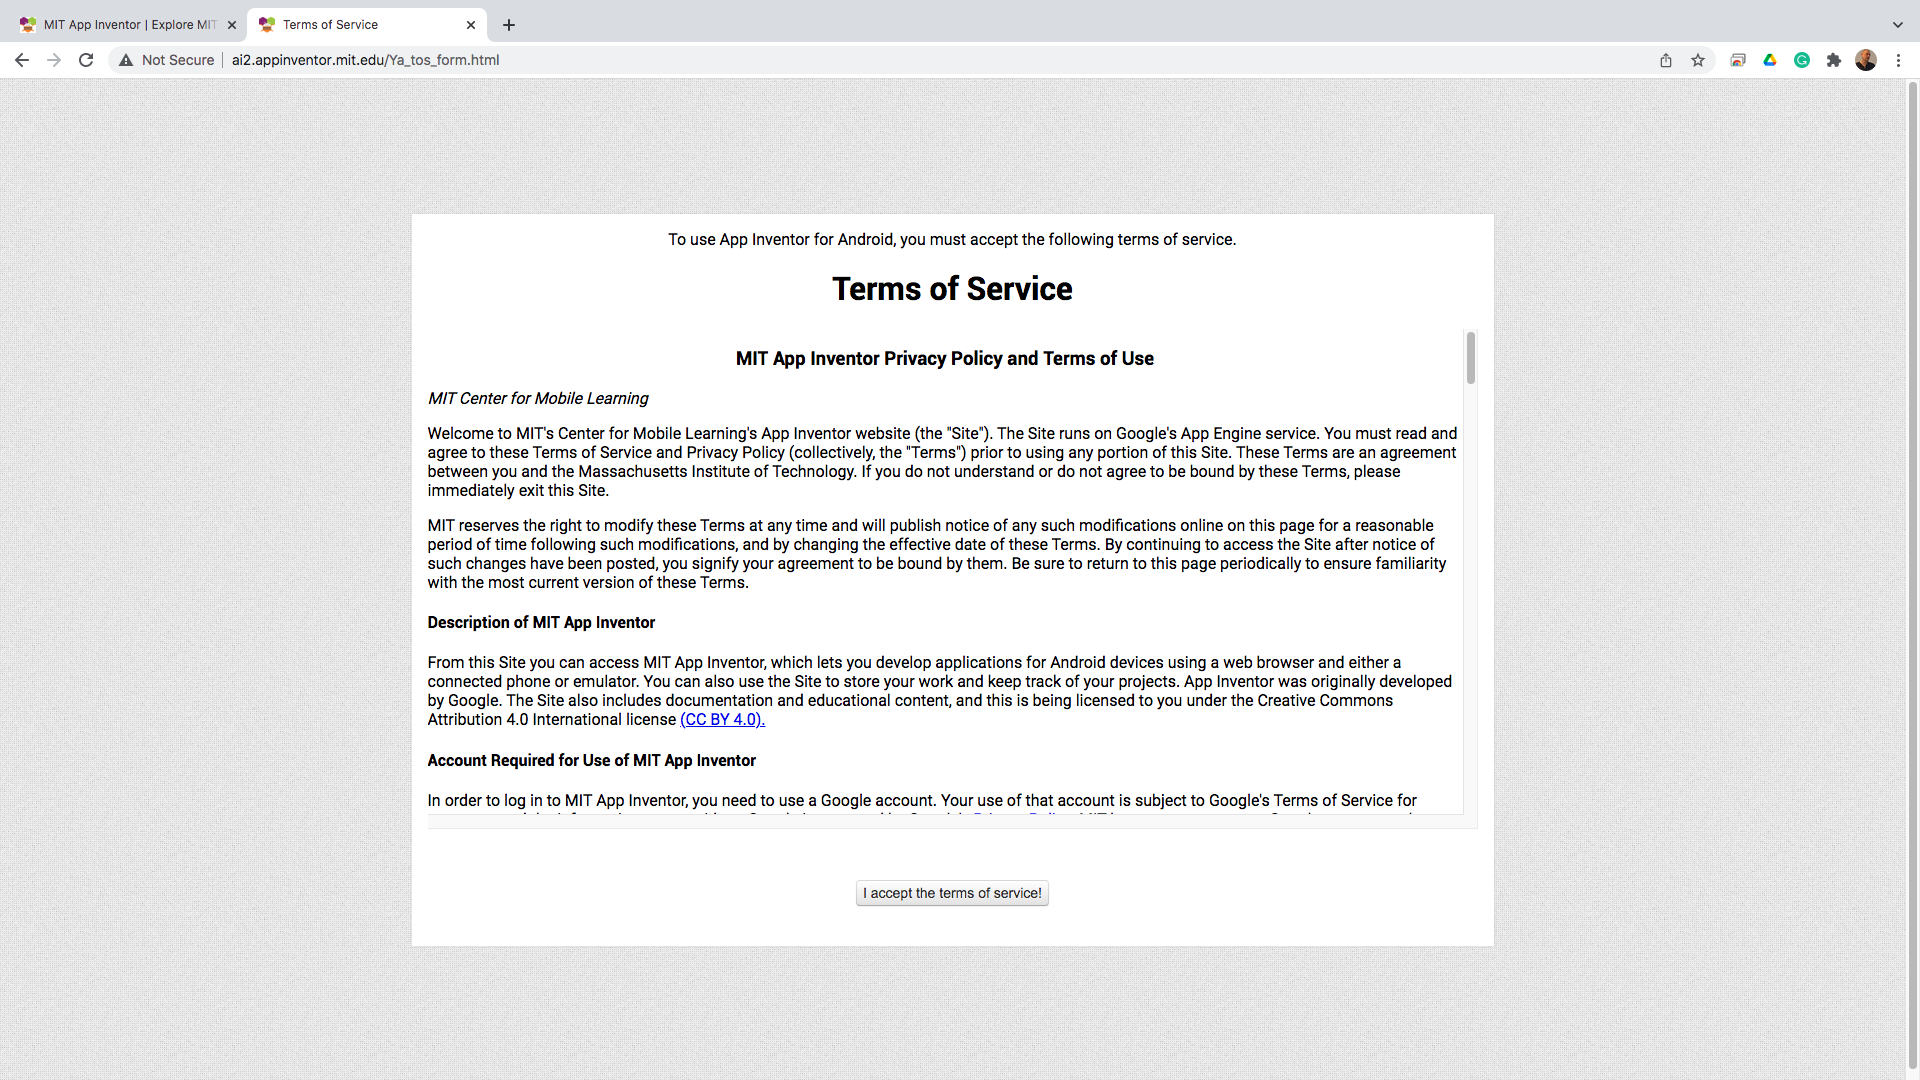
\includegraphics[width=1.0\linewidth,height=0.5\linewidth]{fig010024.png}
   \caption{General Terms of Use of the Program Environment}
\label{fig010024}
\end{figure}

Entering the programming environment ends with a welcome web page (Fig. \ref{fig010025}). This page presents more detailed information about the program environment, the type of instance launched, and the version.

\begin{figure}[H]
   \centering
   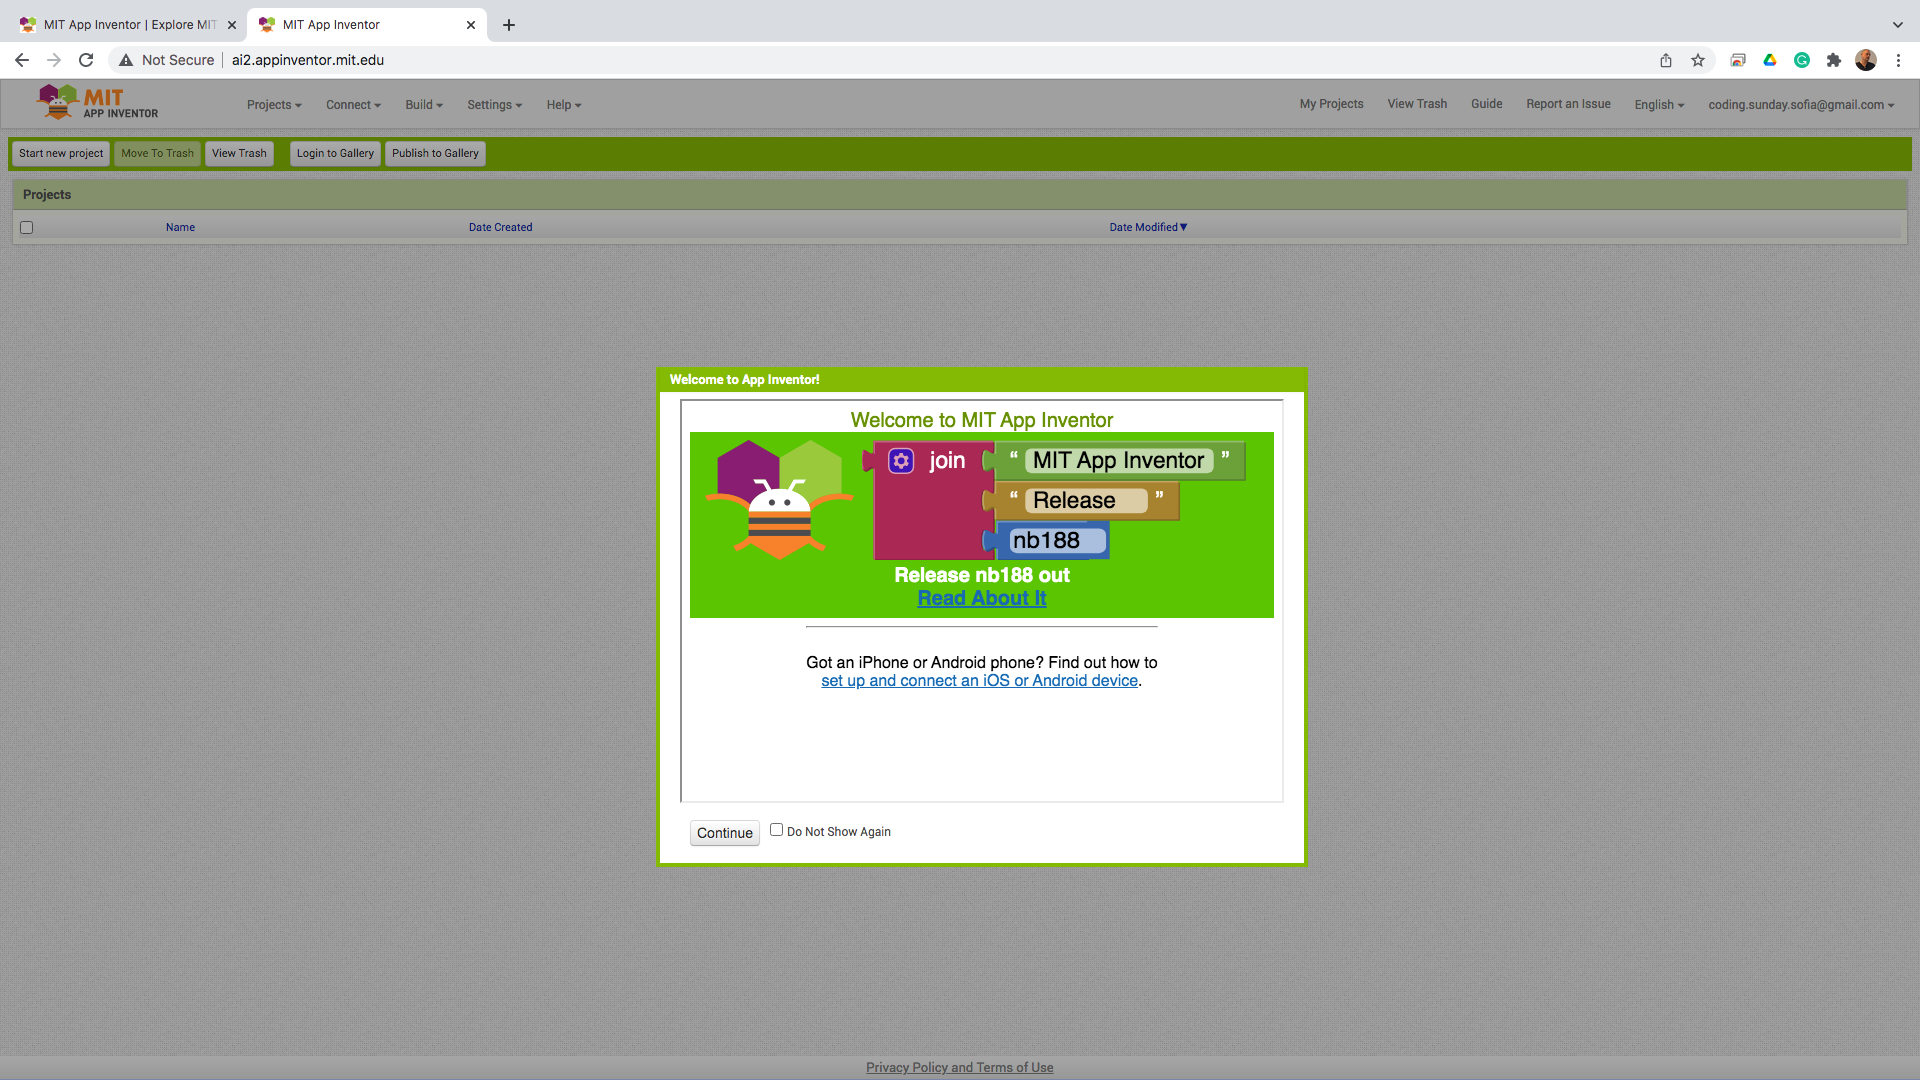
\includegraphics[width=1.0\linewidth,height=0.5\linewidth]{fig010025.png}
   \caption{Welcome Page}
\label{fig010025}
\end{figure}

The first option offered to the user is to choose from options to view several learning projects as an initial introduction to how to work with the programming environment (Fig. \ref{fig010026}).

\begin{figure}[H]
   \centering
   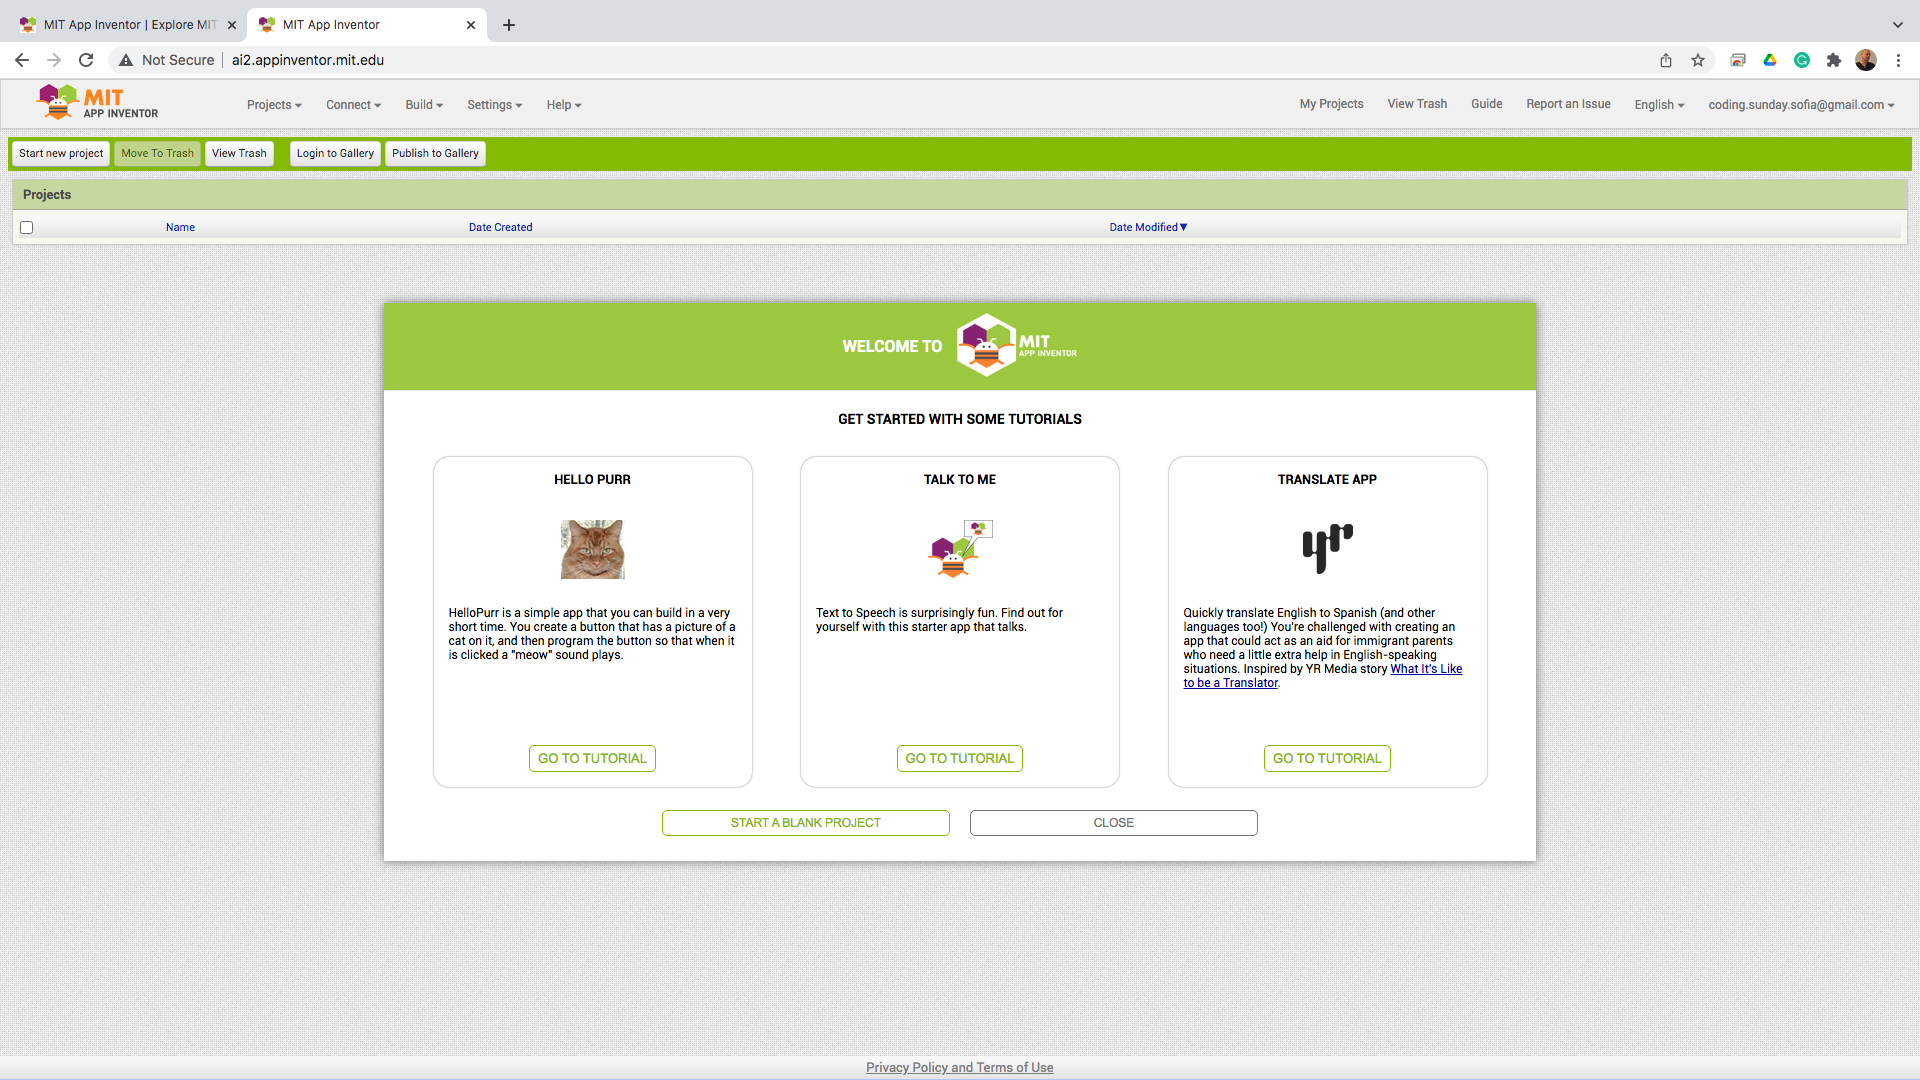
\includegraphics[width=1.0\linewidth,height=0.5\linewidth]{fig010026.png}
   \caption{Ability to choose learning projects}
\label{fig010026}
\end{figure}

If no learning project or the option to create an empty project is selected, the system directs the user to the page with a list of own projects (Fig. \ref{fig010027}).

\begin{figure}[H]
   \centering
   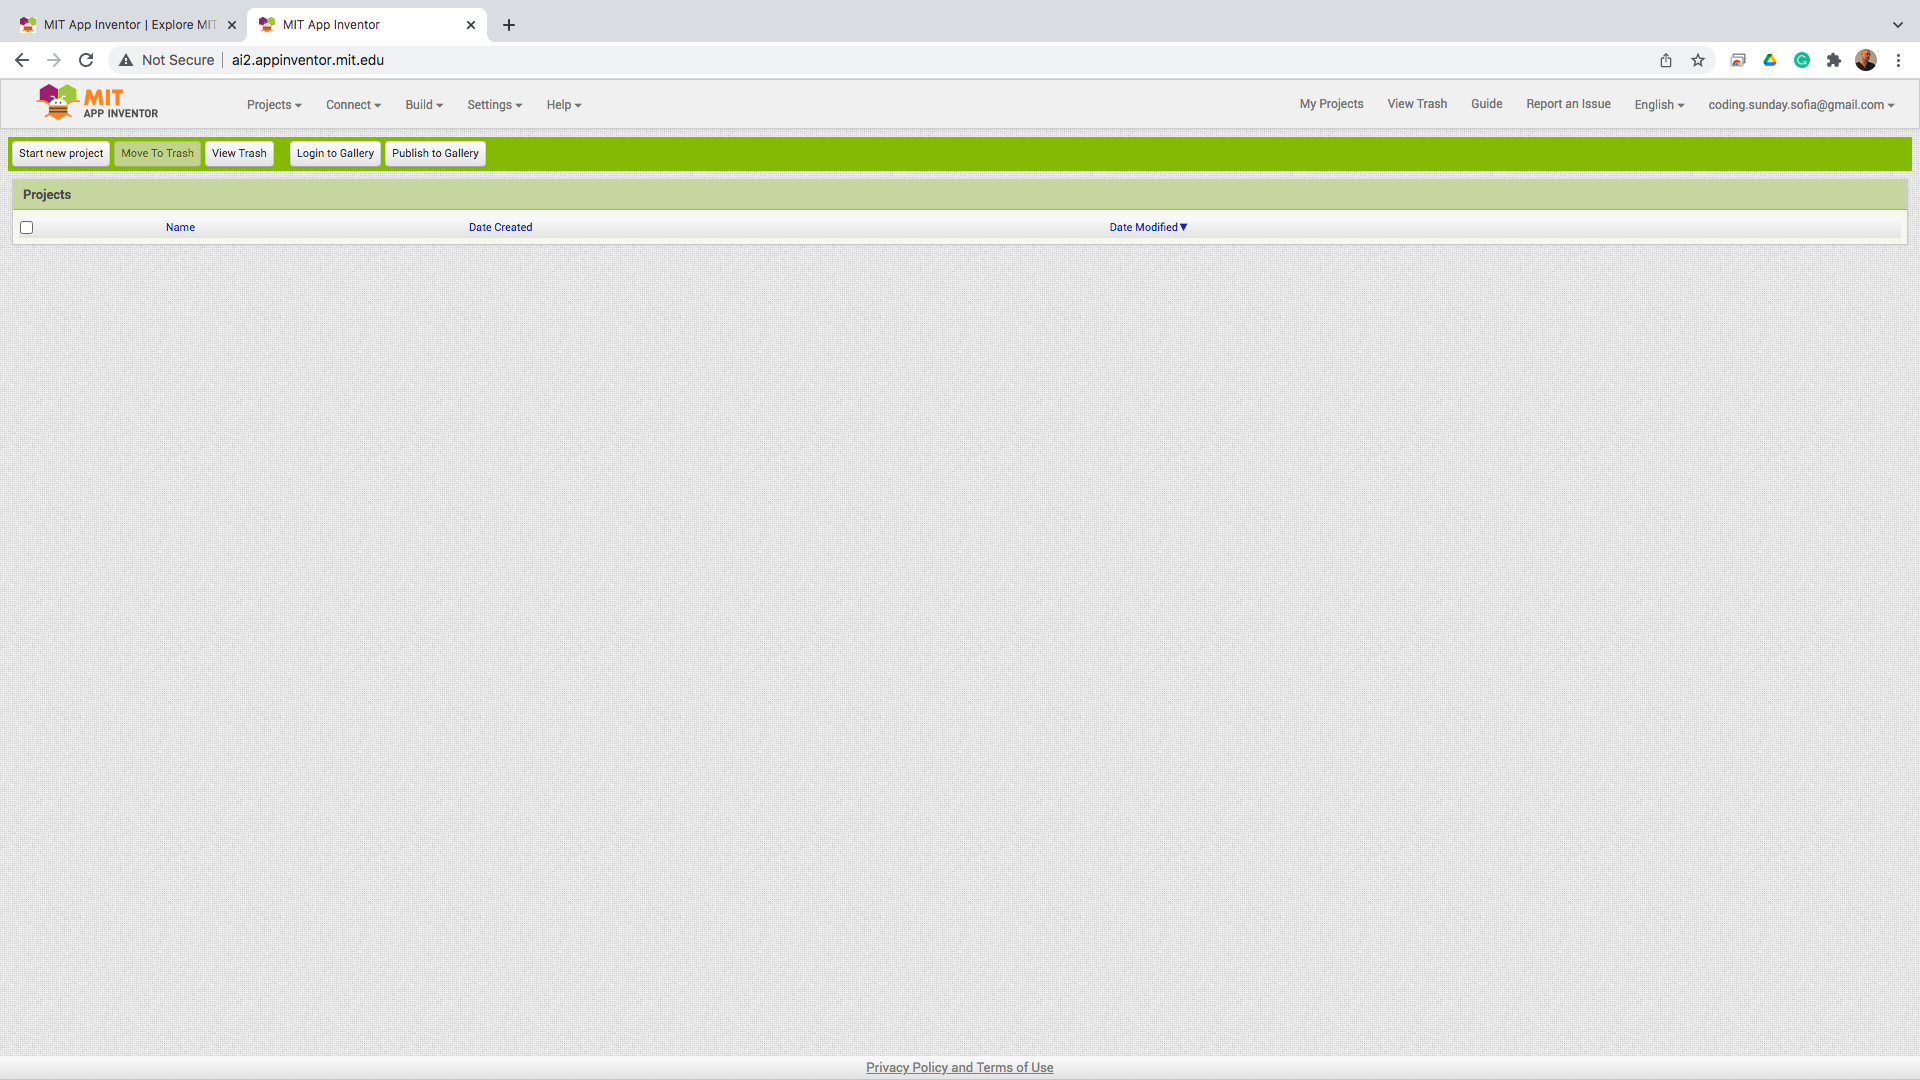
\includegraphics[width=1.0\linewidth,height=0.5\linewidth]{fig010027.png}
   \caption{Own Projects List Page}
\label{fig010027}
\end{figure}

Starting a new project happens from a button, at the top left, on the main work screen (Fig. \ref{fig010028}).

\begin{figure}[H]
   \centering
   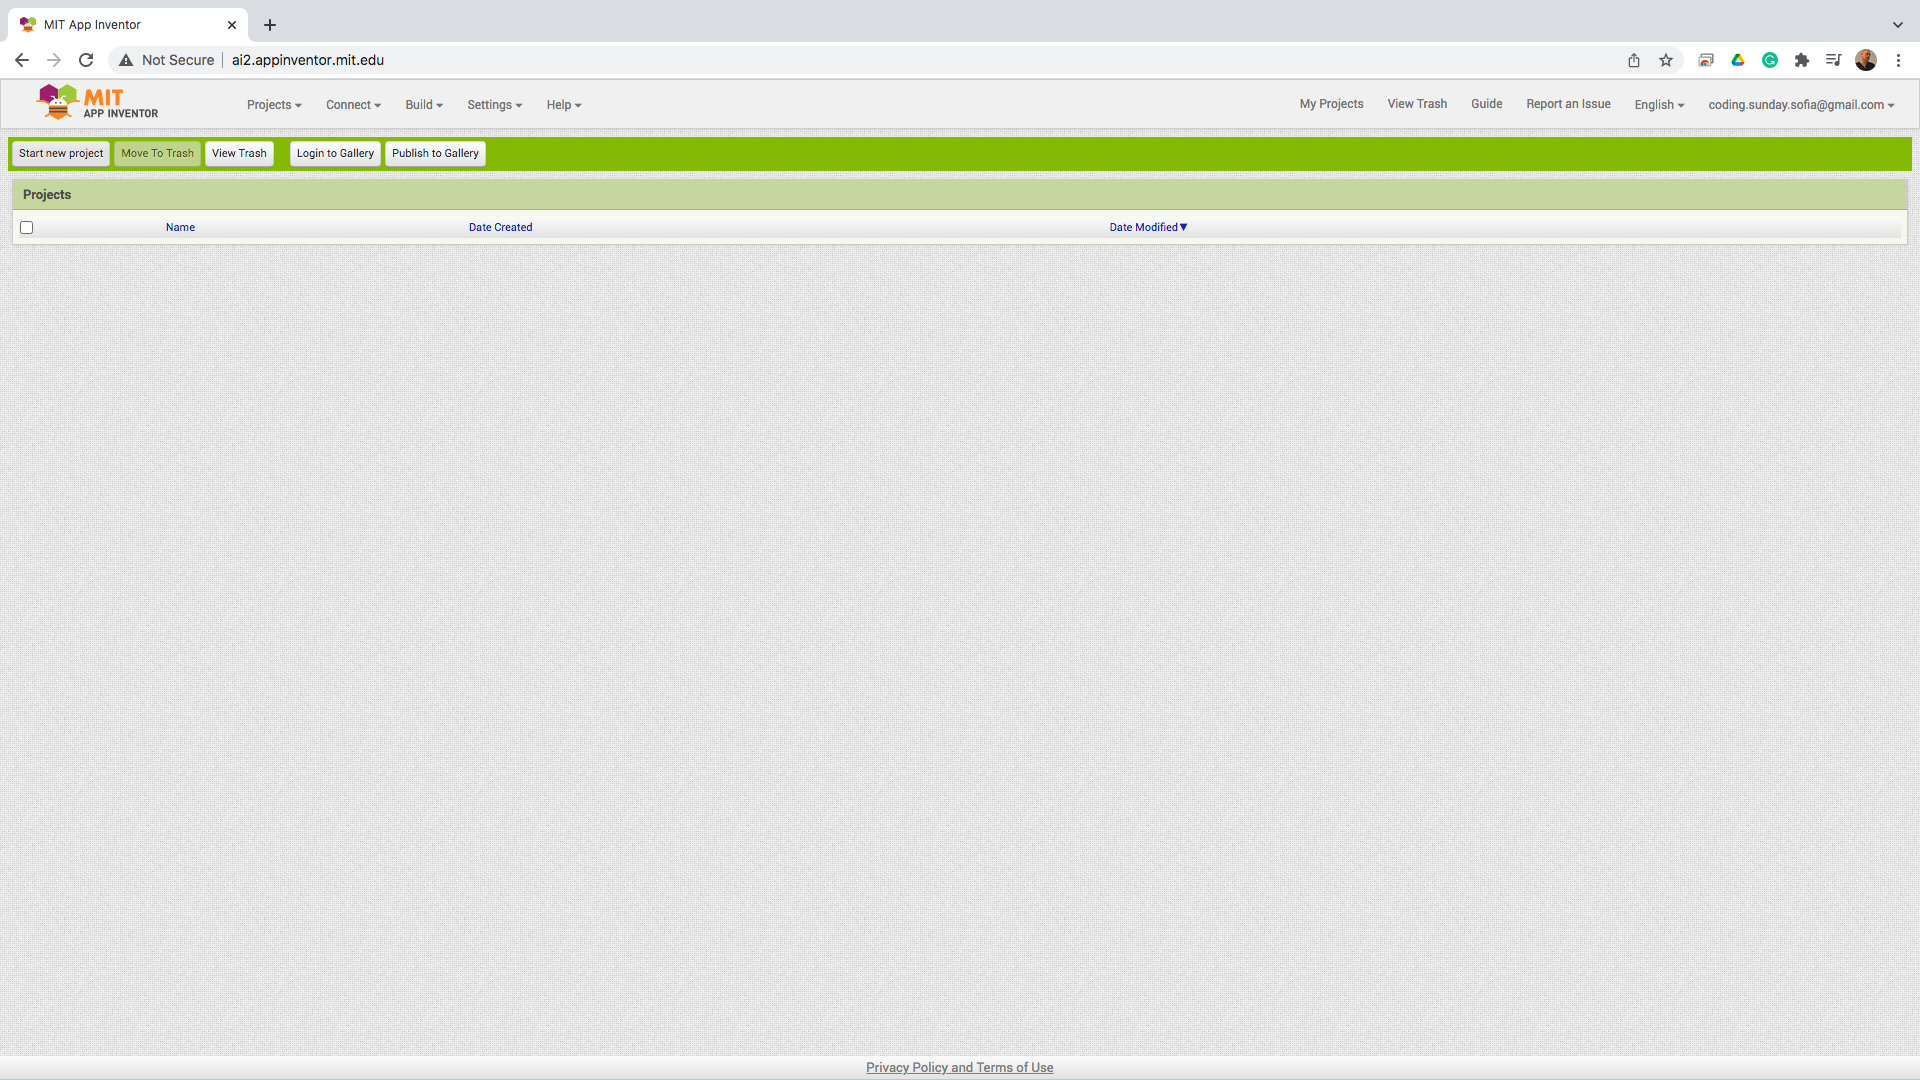
\includegraphics[width=1.0\linewidth,height=0.5\linewidth]{fig010028.png}
   \caption{Start New Project Button}
\label{fig010028}
\end{figure}

The App Inventor programming environment organizes work on programming code through projects. Each project must have an appropriate name set when the project is created (Fig. \ref{fig010029}).

\begin{figure}[H]
   \centering
   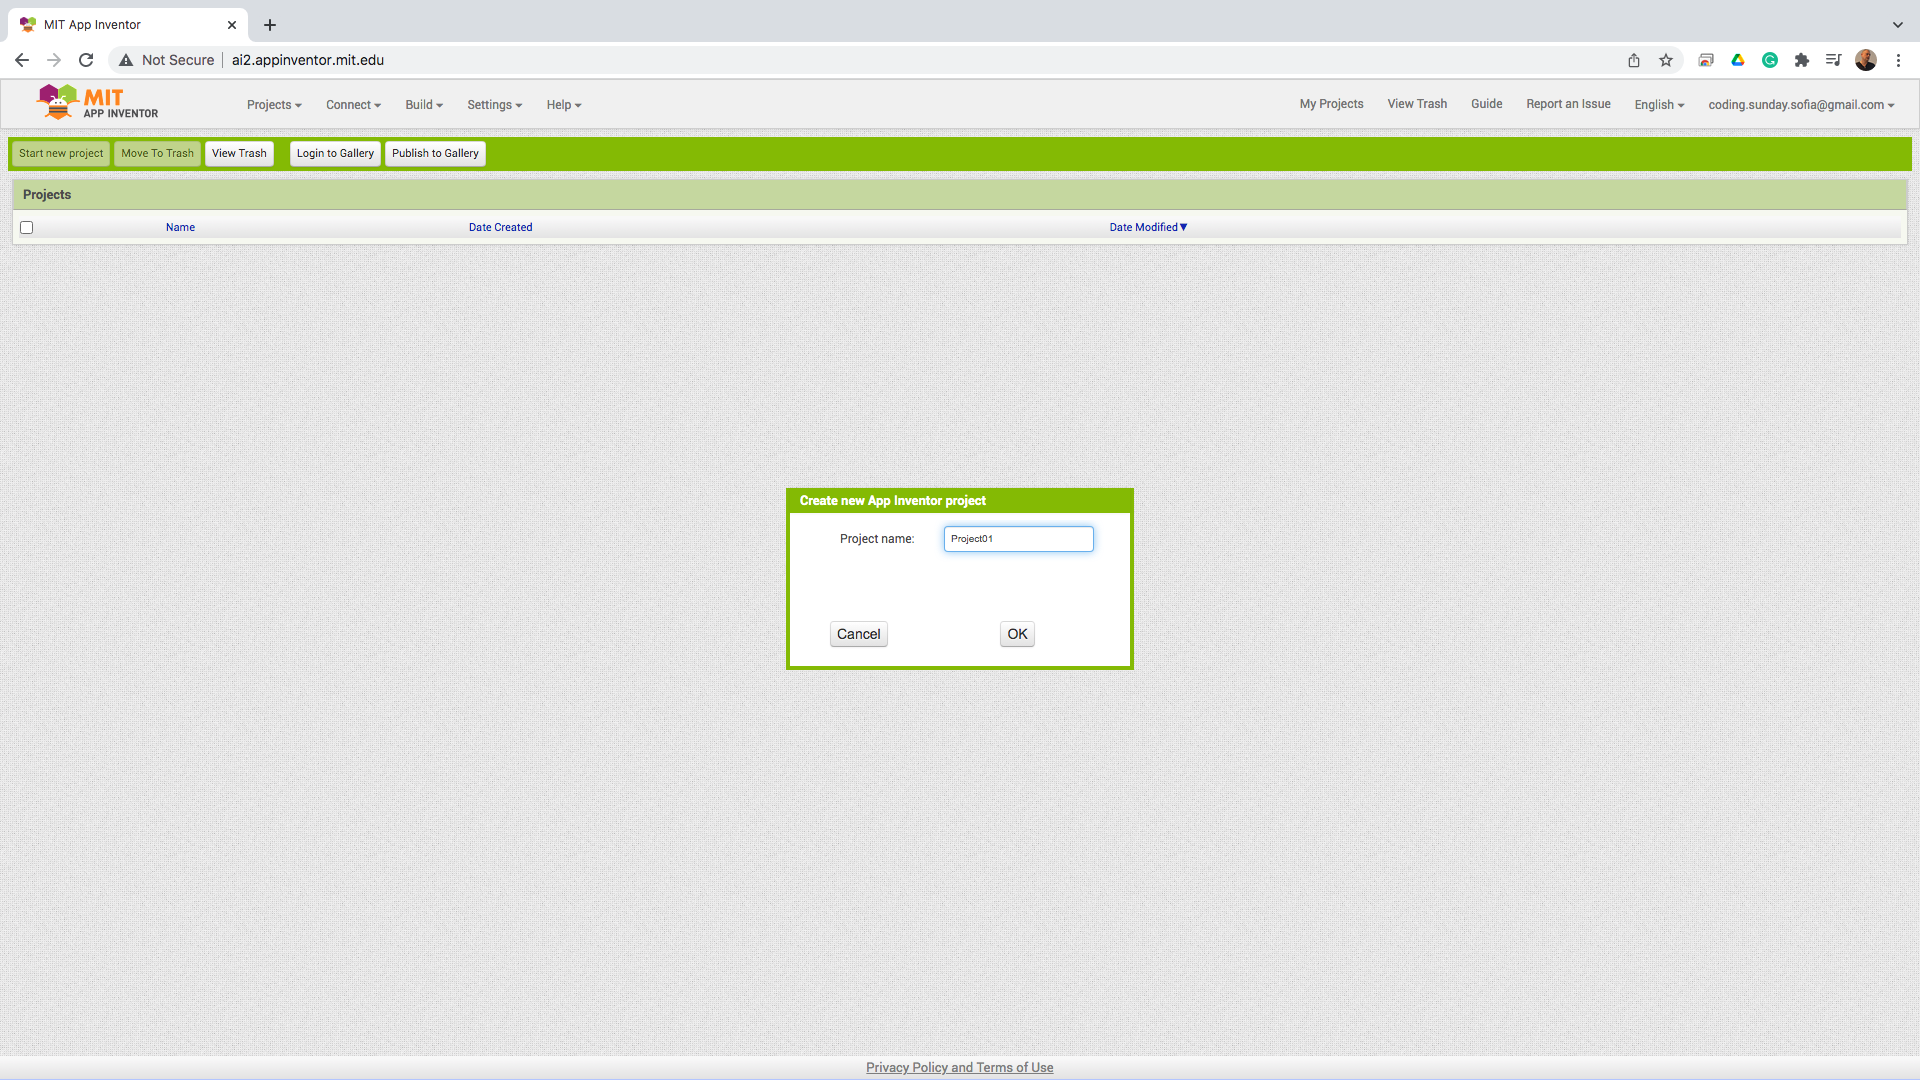
\includegraphics[width=1.0\linewidth,height=0.5\linewidth]{fig010029.png}
   \caption{Project Name}
\label{fig010029}
\end{figure}

After choosing a name, the programming environment visualizes the first working screen, giving the possibility to design the visual user interface (Fig. \ref{fig010030}). Creating the graphical user interface happens by dragging the various visual controls into the main work area.

\begin{figure}[H]
   \centering
   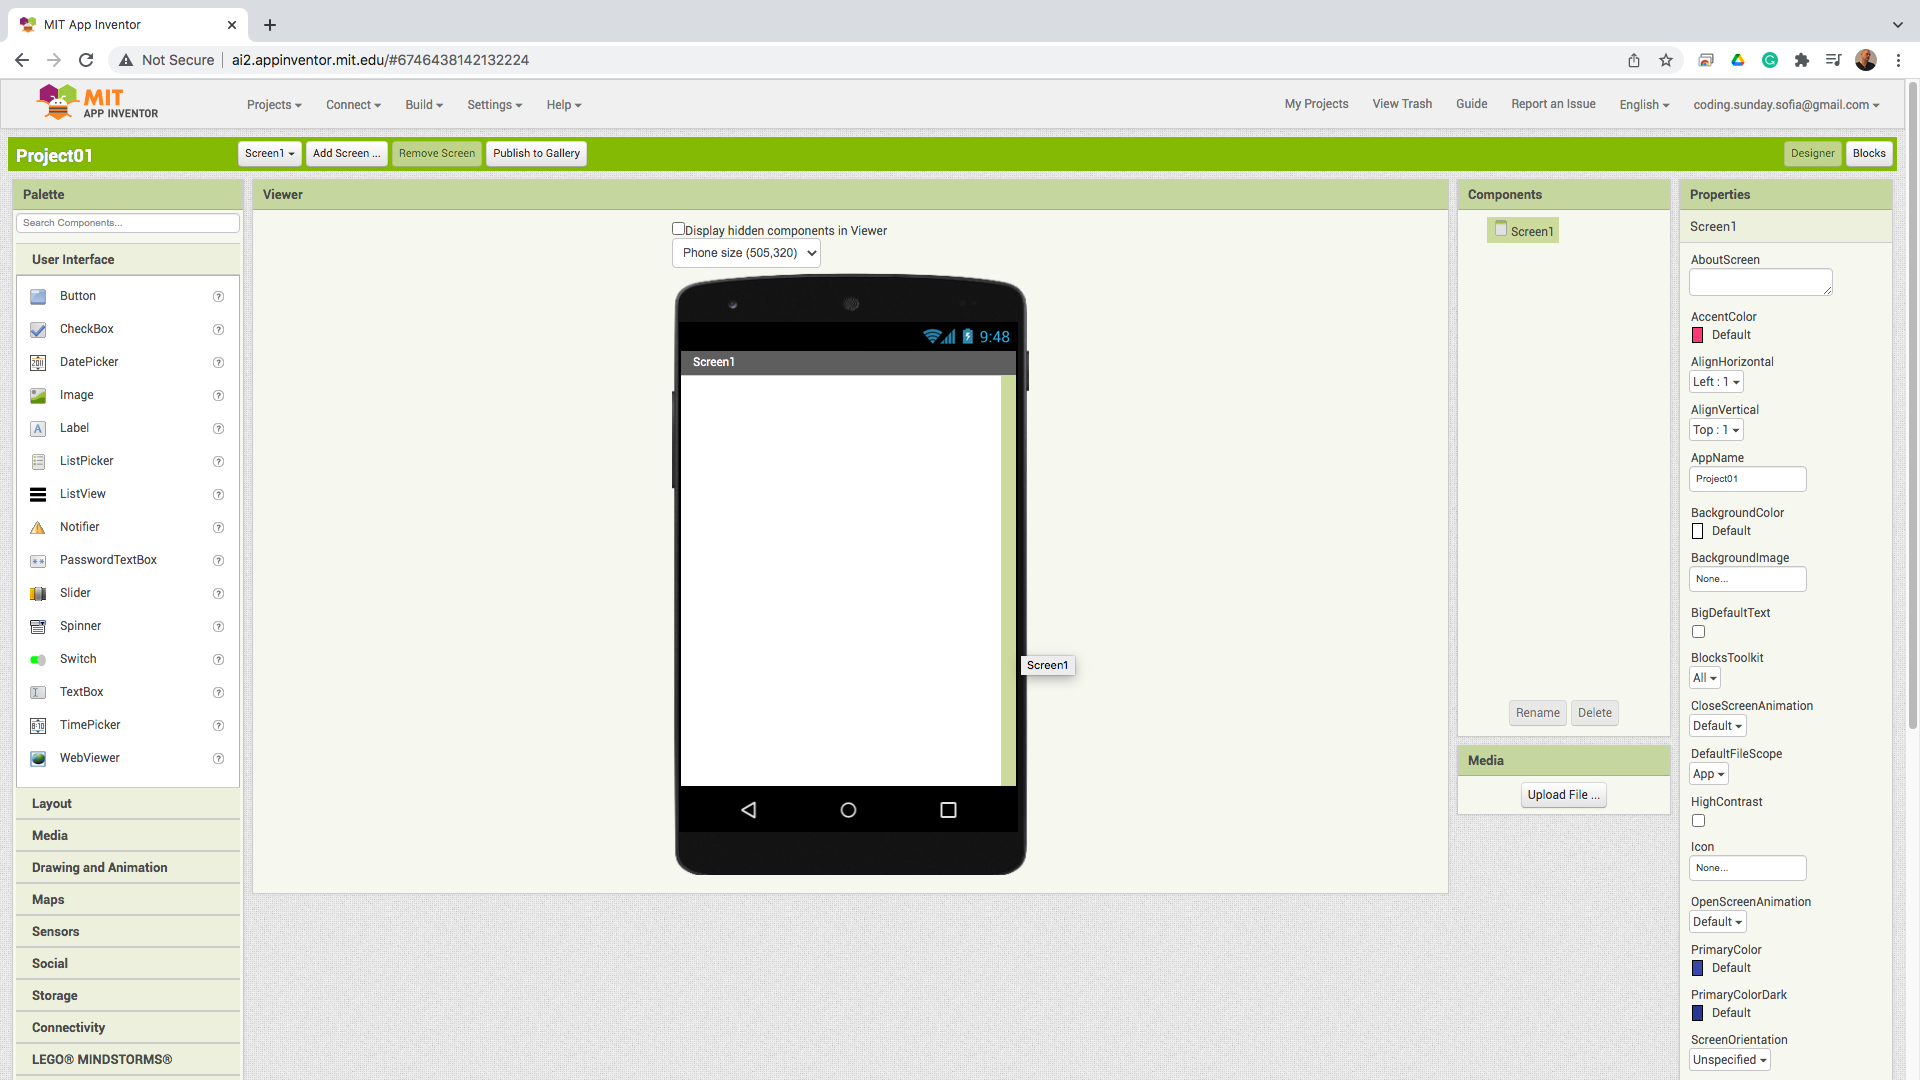
\includegraphics[width=1.0\linewidth,height=0.5\linewidth]{fig010030.png}
   \caption{Design view of the development environment}
\label{fig010030}
\end{figure}

One of the most basic visual controls is the button. Represents a designated area in the visual field with a text label or icon to visually represent the action performed after the button is pressed. One button is used to demonstrate the process of working with the compiled program code (Fig. \ref{fig010031}).

\begin{figure}[H]
   \centering
   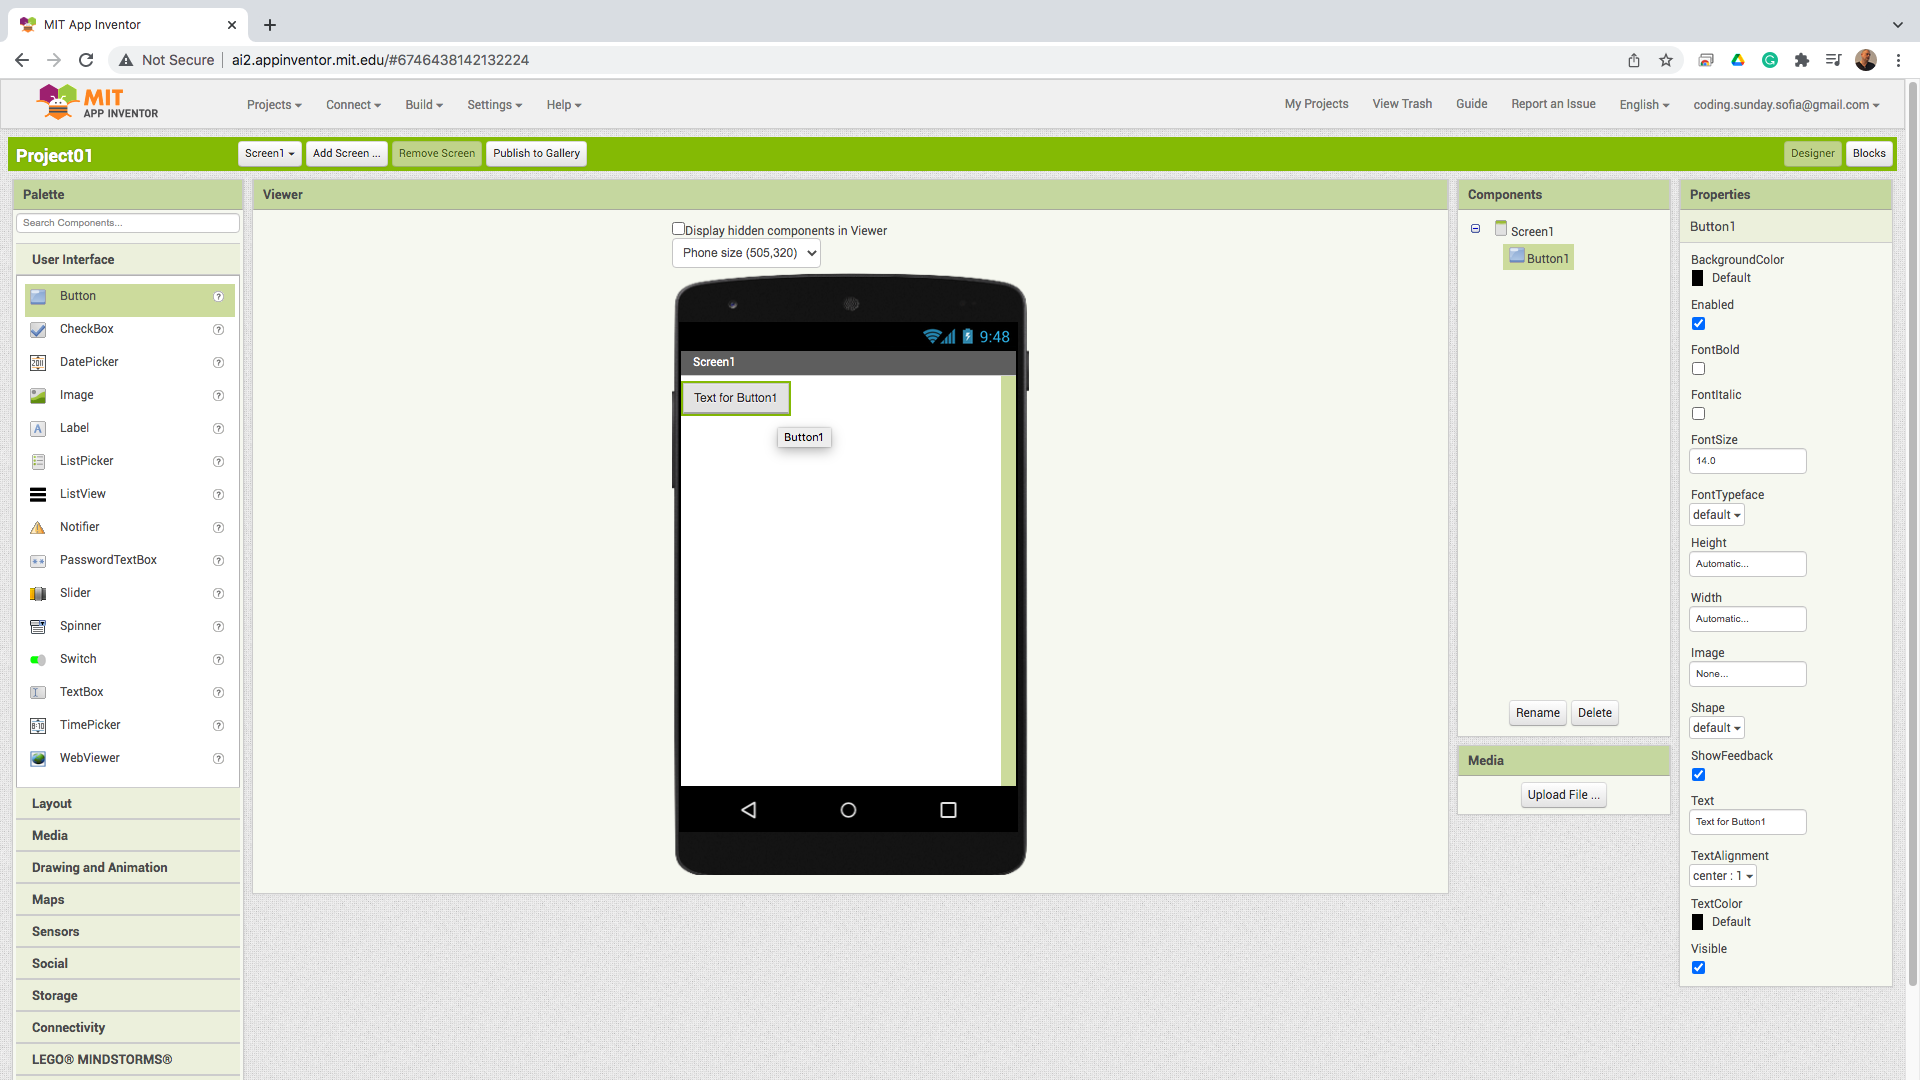
\includegraphics[width=1.0\linewidth,height=0.5\linewidth]{fig010031.png}
   \caption{Place Button}
\label{fig010031}
\end{figure}

It is essential for people using the software application that the buttons have maximally expressive names. In this case, the goal is for the button to be pressed and a specific action to follow. For this reason, the name of the button is just "Push" (Fig. \ref{fig010031}).

\begin{figure}[H]
   \centering
   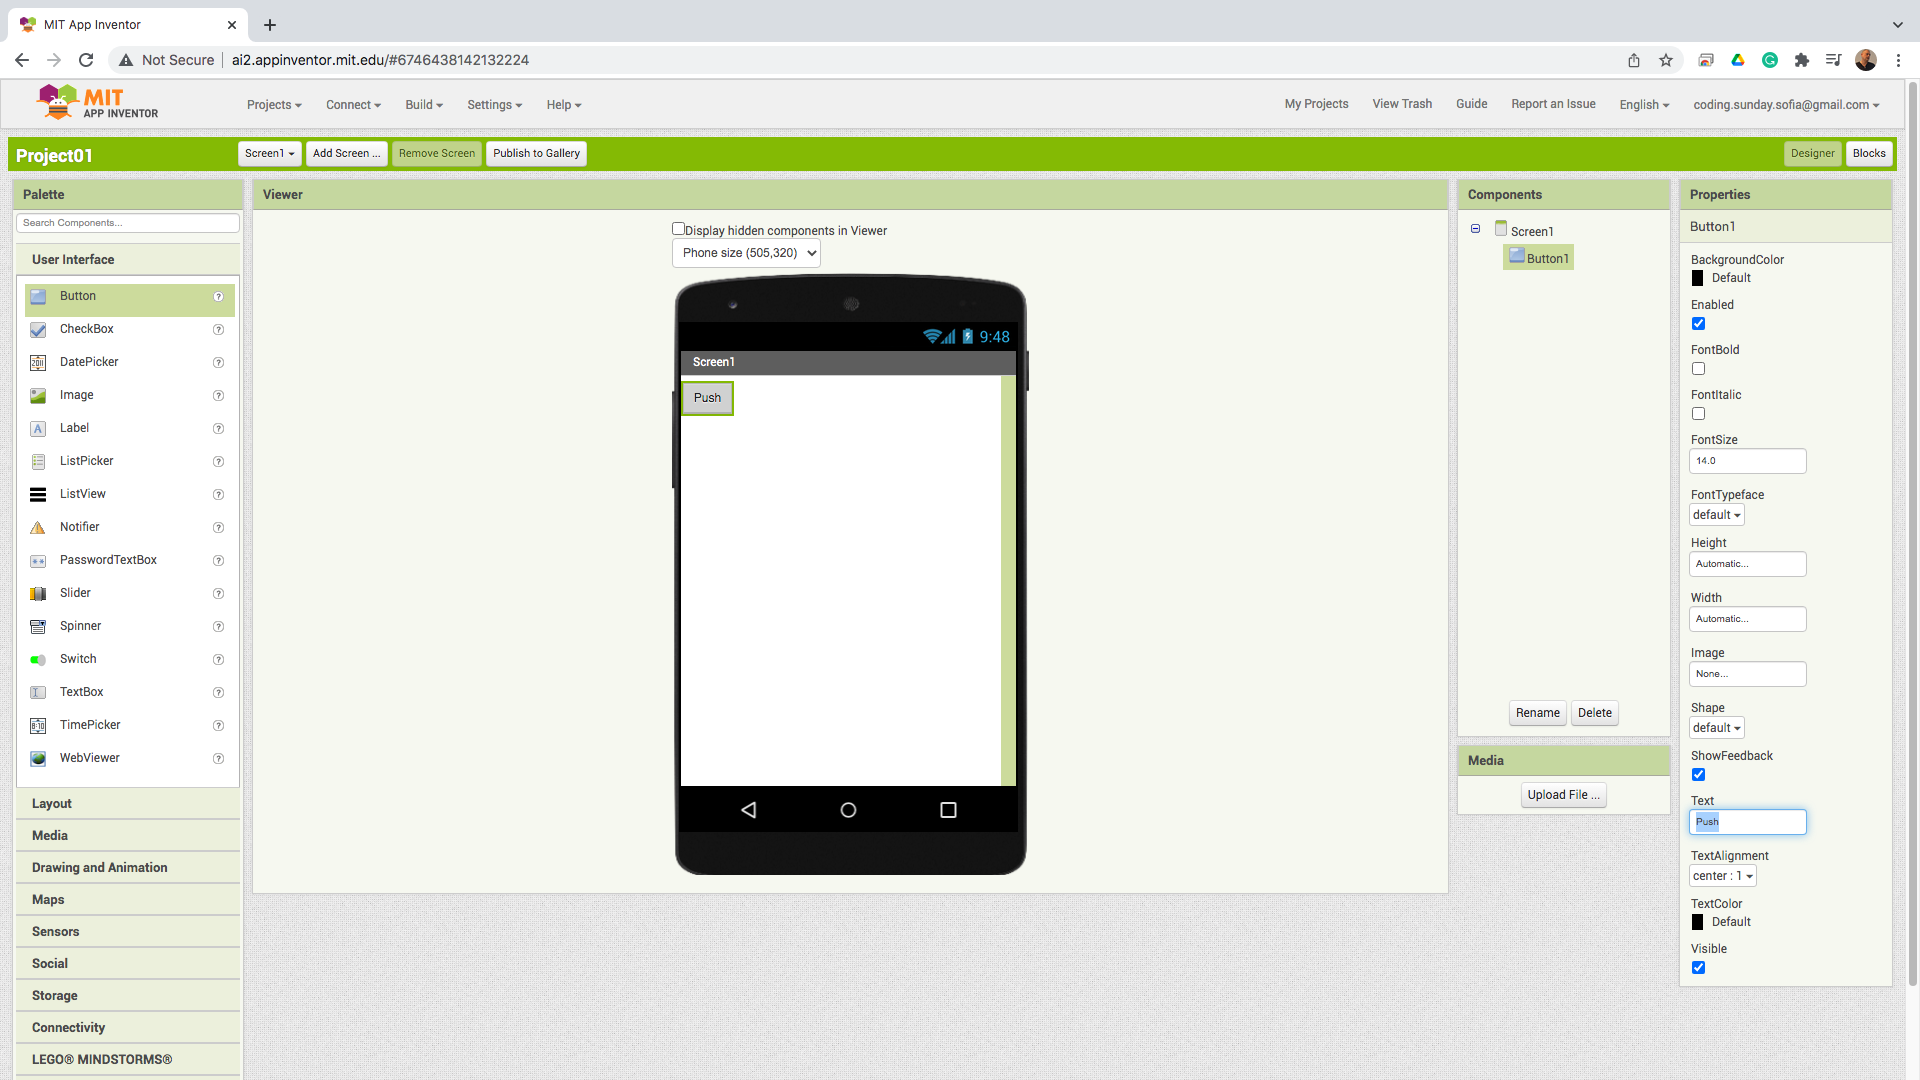
\includegraphics[width=1.0\linewidth,height=0.5\linewidth]{fig010032.png}
   \caption{Select text on button}
\label{fig010032}
\end{figure}

Unlike the Scratch programming environment, App Inventor's program instructions are cut as a puzzle in a separate work screen (Fig. \ref{fig010033}).

\begin{figure}[H]
   \centering
   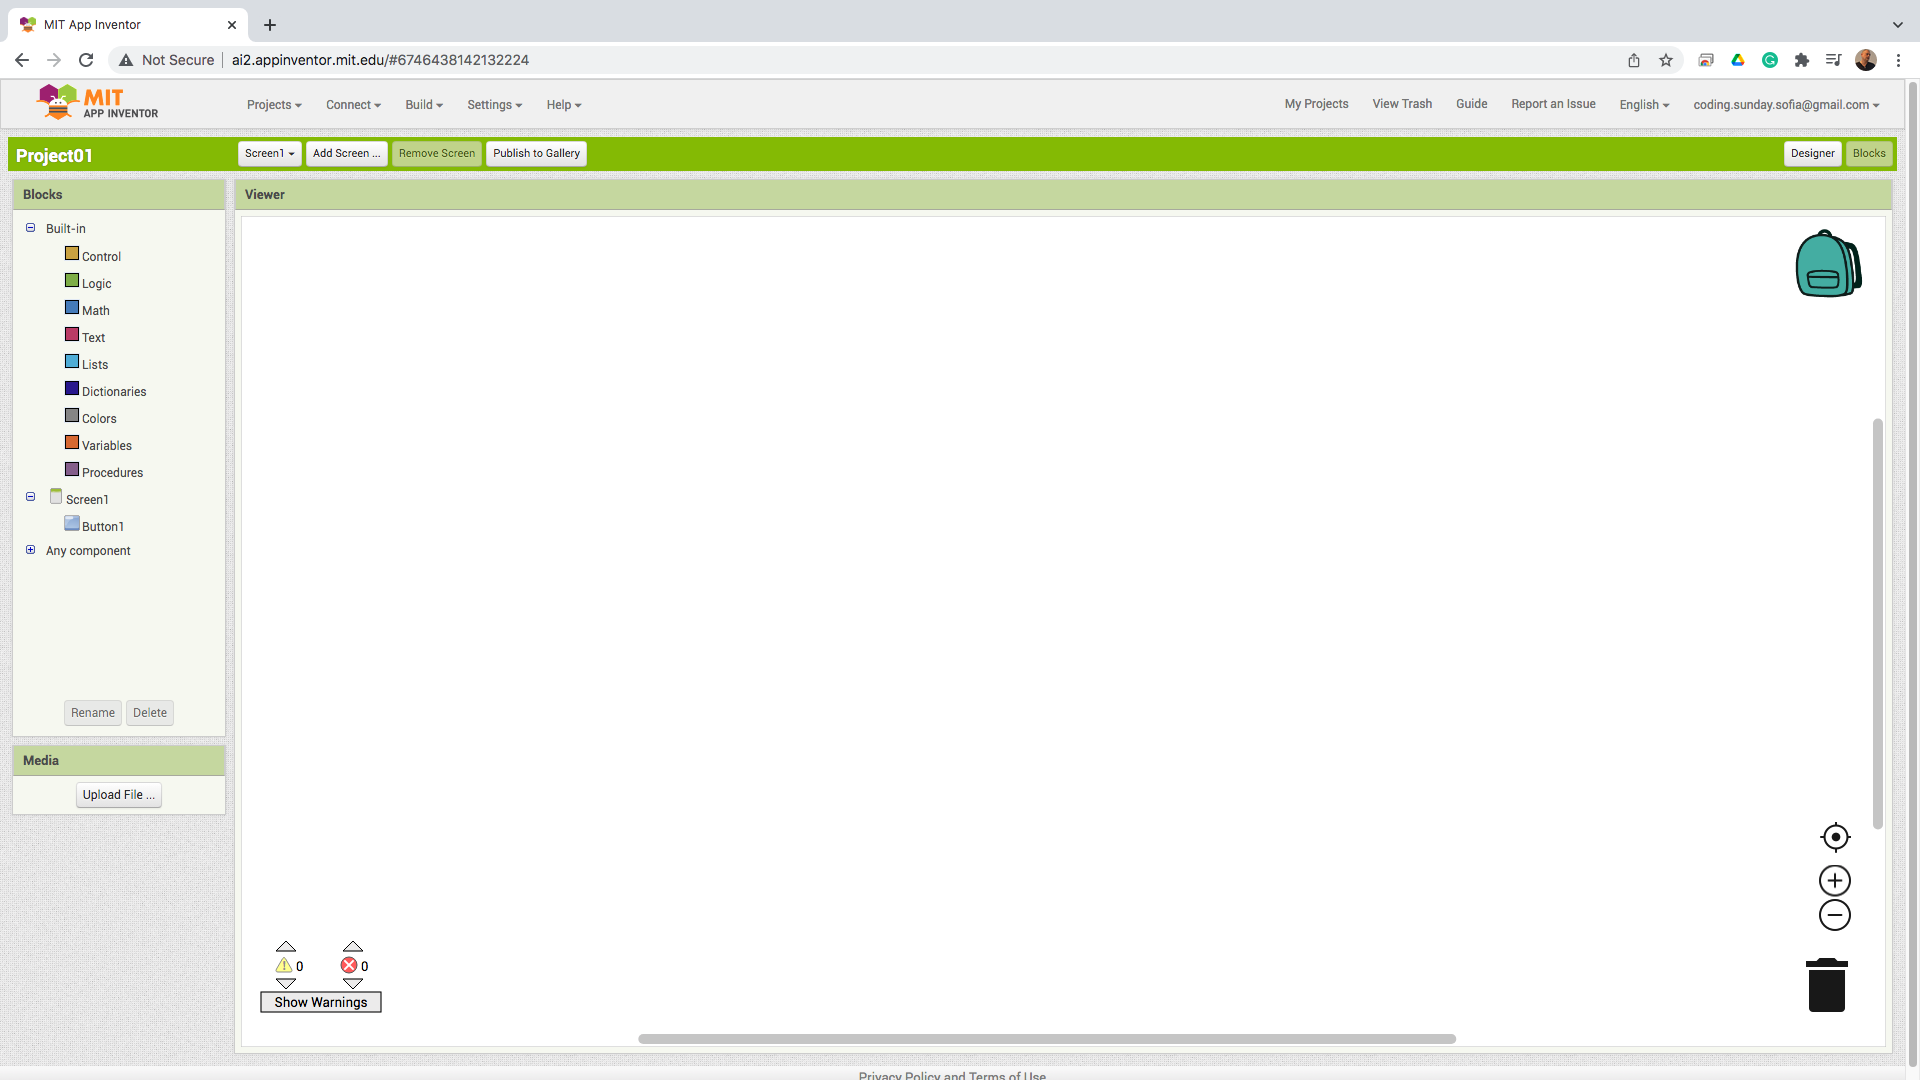
\includegraphics[width=1.0\linewidth,height=0.5\linewidth]{fig010033.png}
   \caption{Program view of the development environment}
\label{fig010033}
\end{figure}

Since the graphical user interface has only a single component (a button), some instructions can only be executed with this visual component. Unlike Scratch, where the program has an initial starting point and a final endpoint, App Inventor's instructions are ordered according to the principle of occurring events. When the program starts running, it visualizes the graphical user interface and expects the device user to perform some action (Fig. \ref{fig010034}).

\begin{figure}[H]
   \centering
   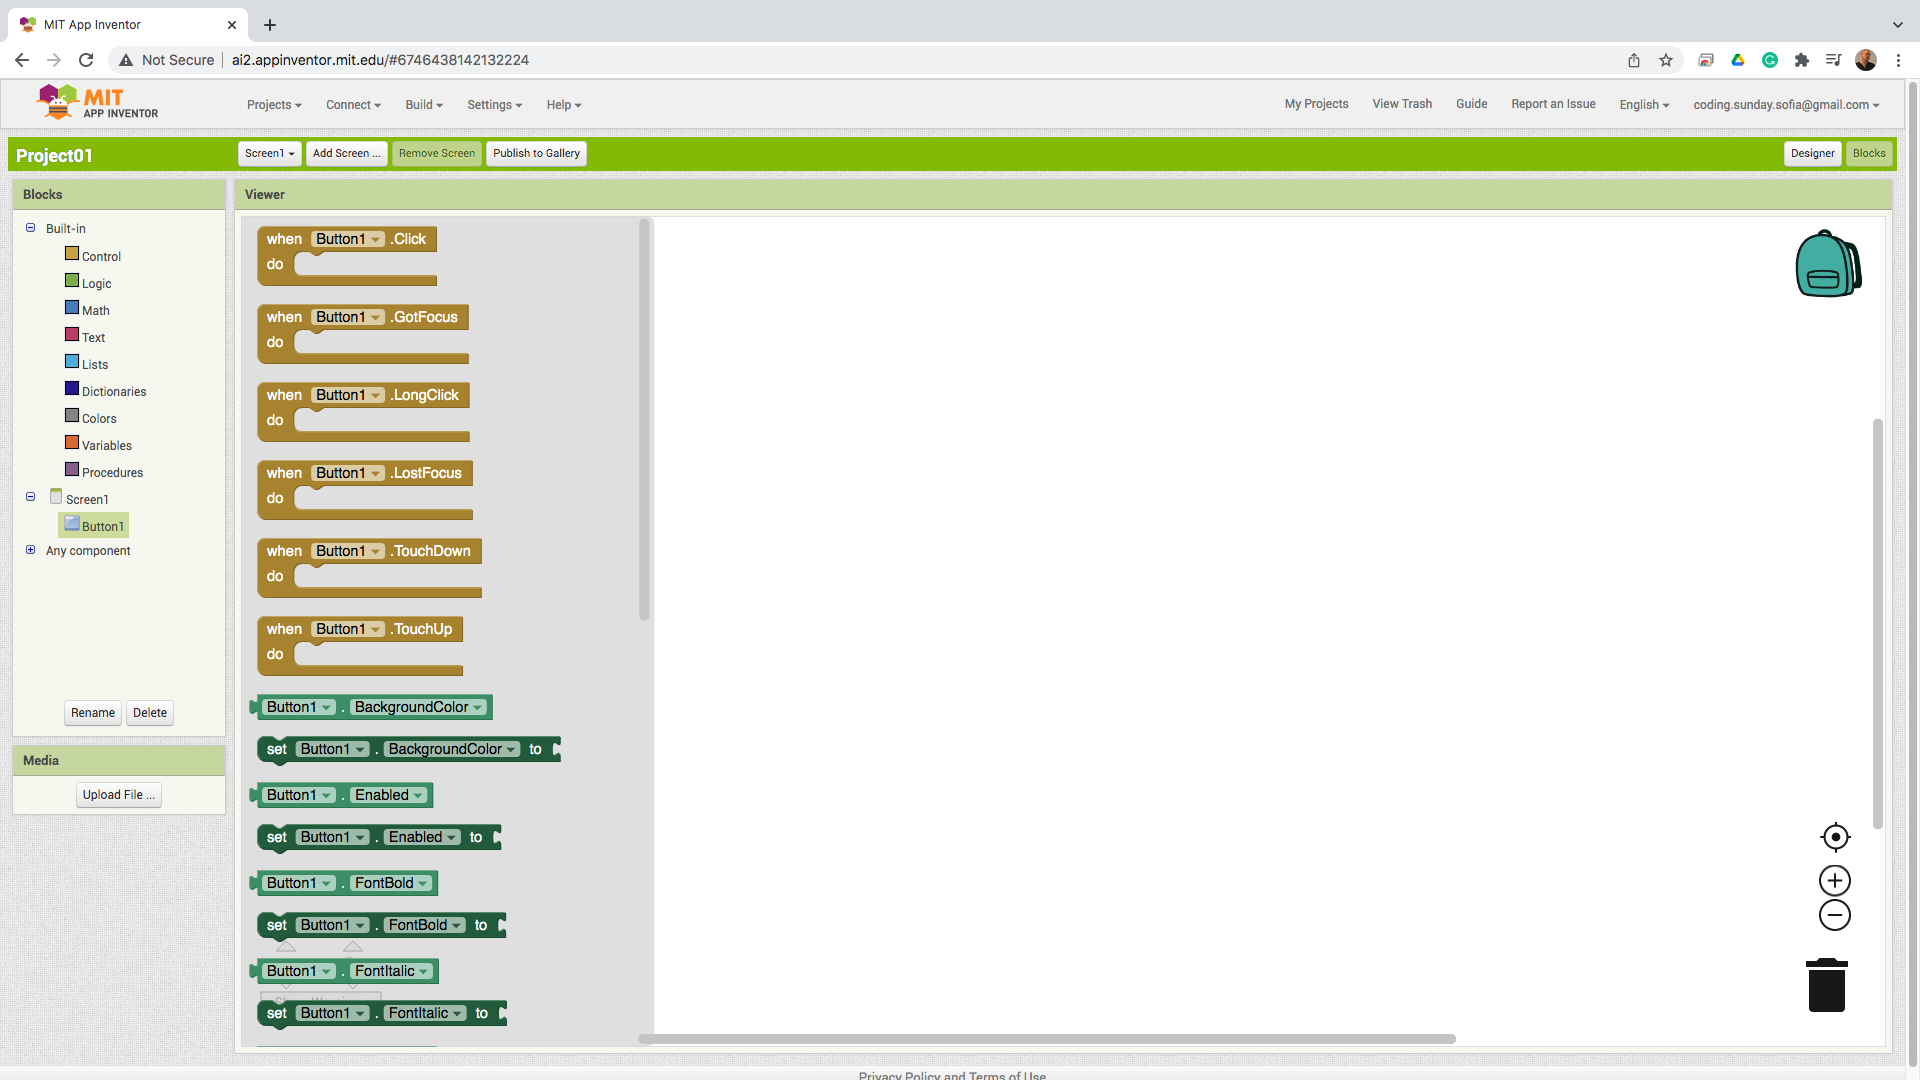
\includegraphics[width=1.0\linewidth,height=0.5\linewidth]{fig010034.png}
   \caption{List of instructions}
\label{fig010034}
\end{figure}

Such an action could be pressing a button. On the App Inventor side, the pressed button generates an event (event), for which event-specific activities of the program are selected (Fig. \ref{fig010035}).

\begin{figure}[H]
   \centering
   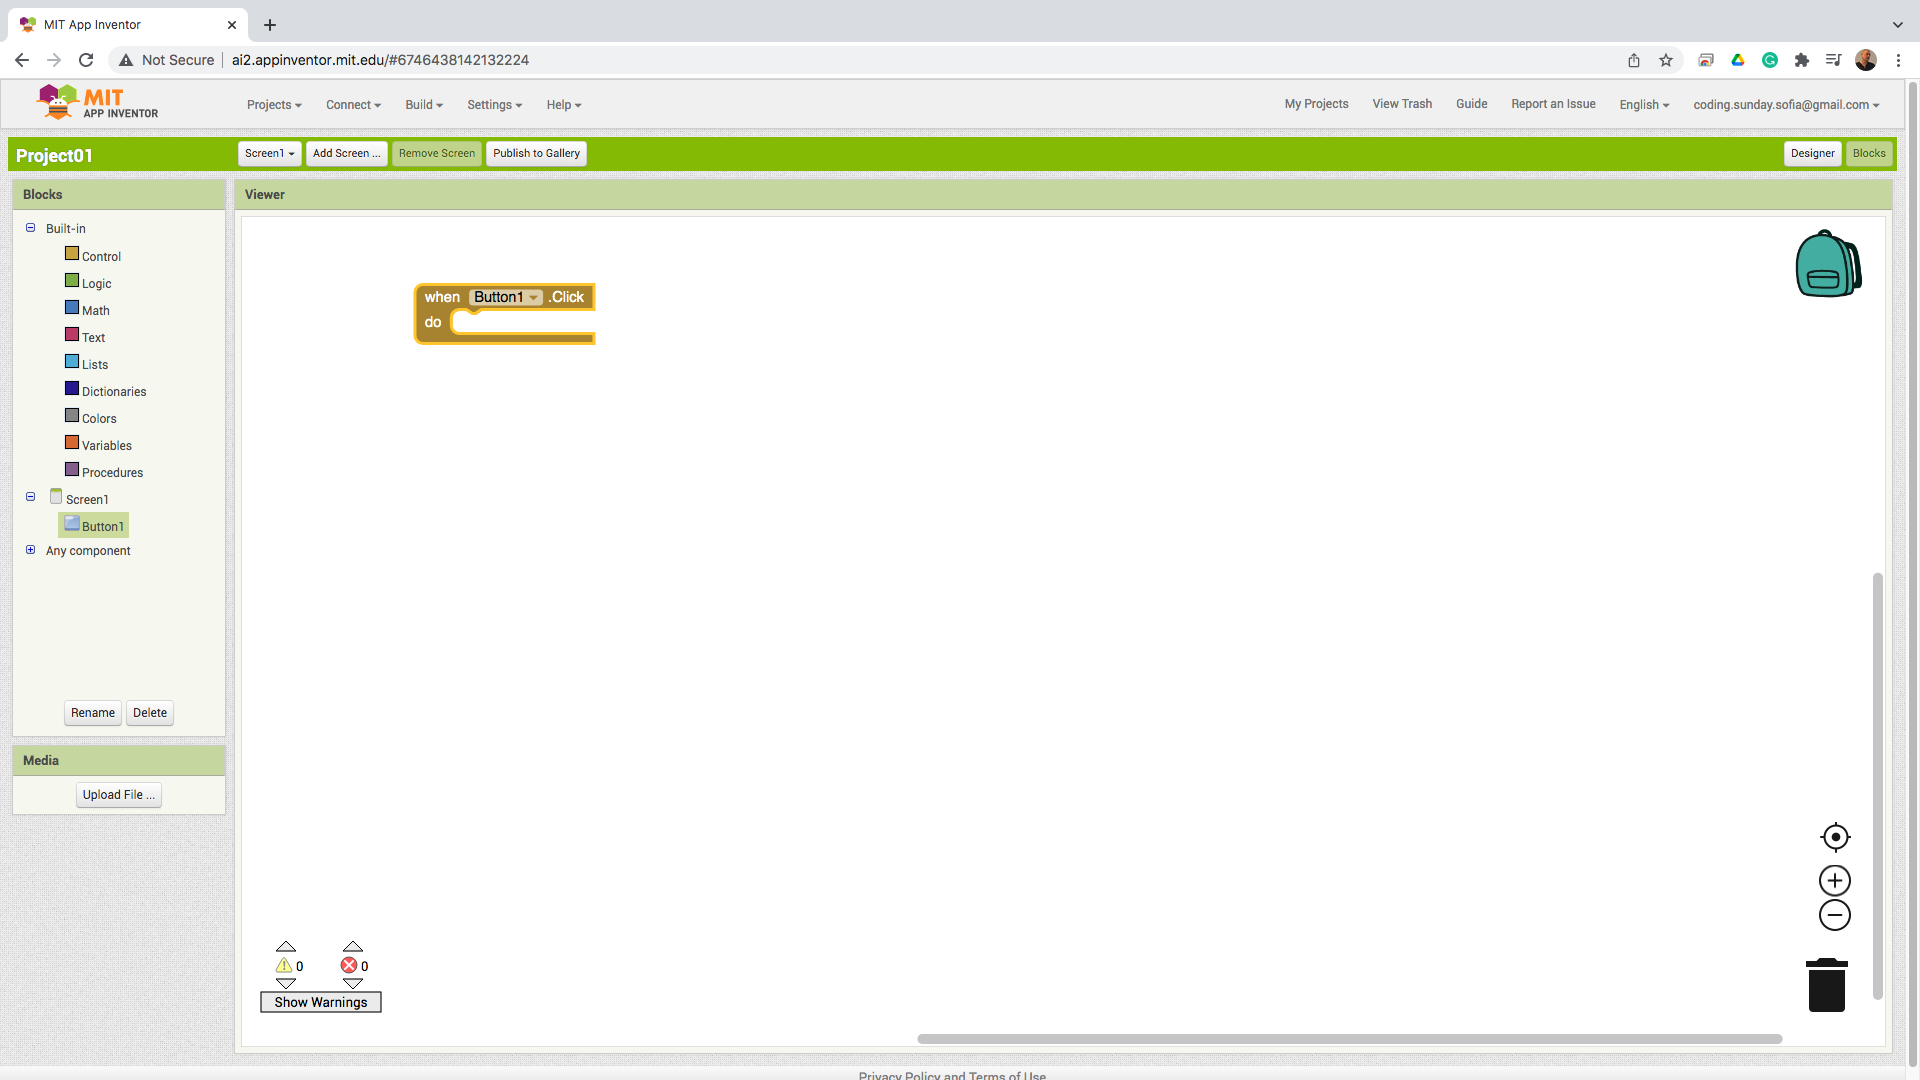
\includegraphics[width=1.0\linewidth,height=0.5\linewidth]{fig010035.png}
   \caption{Select event for button press}
\label{fig010035}
\end{figure}

The button press event is visualized as a puzzle piece containing a slot into which the instructions to be executed can be arranged (Fig. \ref{fig010036}).

\begin{figure}[H]
   \centering
   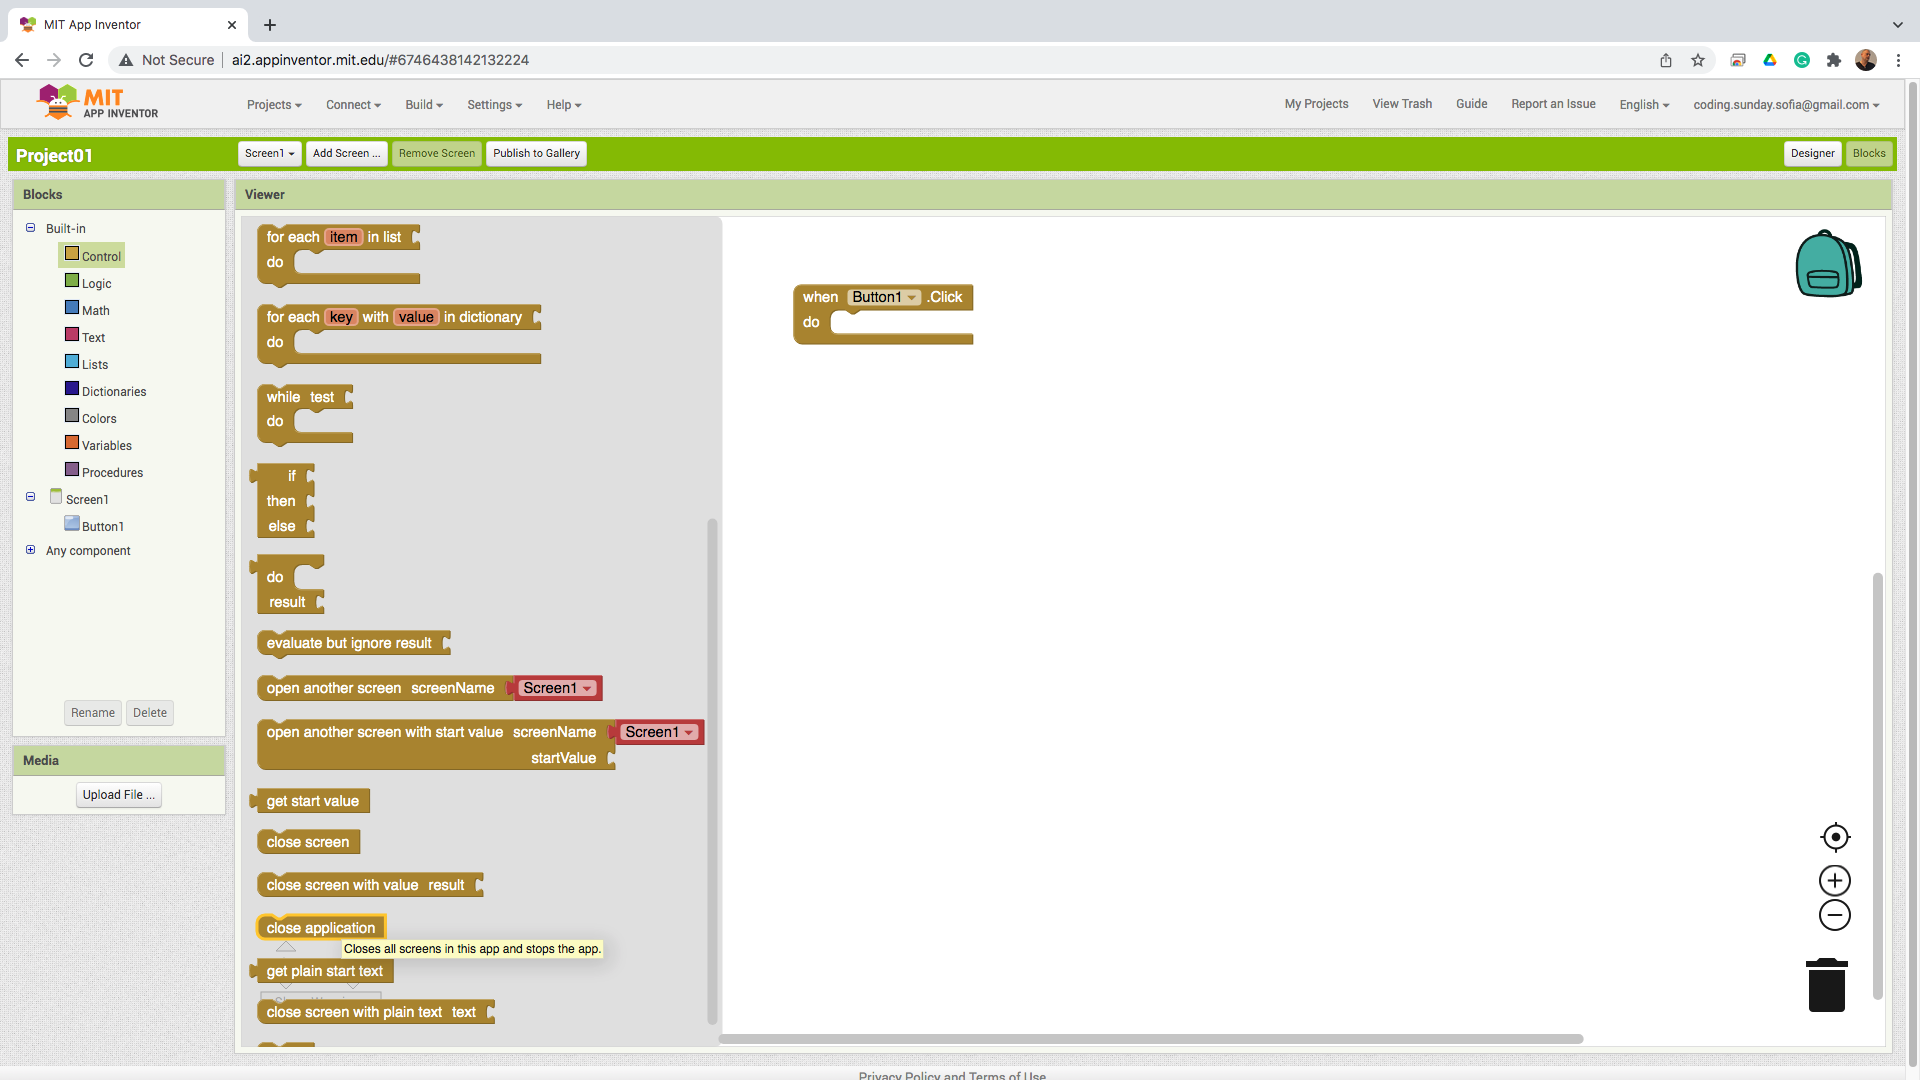
\includegraphics[width=1.0\linewidth,height=0.5\linewidth]{fig010036.png}
   \caption{Select action when the button is pressed}
\label{fig010036}
\end{figure}

The most straightforward action that can be performed after pressing the button is to stop the program and close the window of the application being developed (Fig. \ref{fig010037}).

\begin{figure}[H]
   \centering
   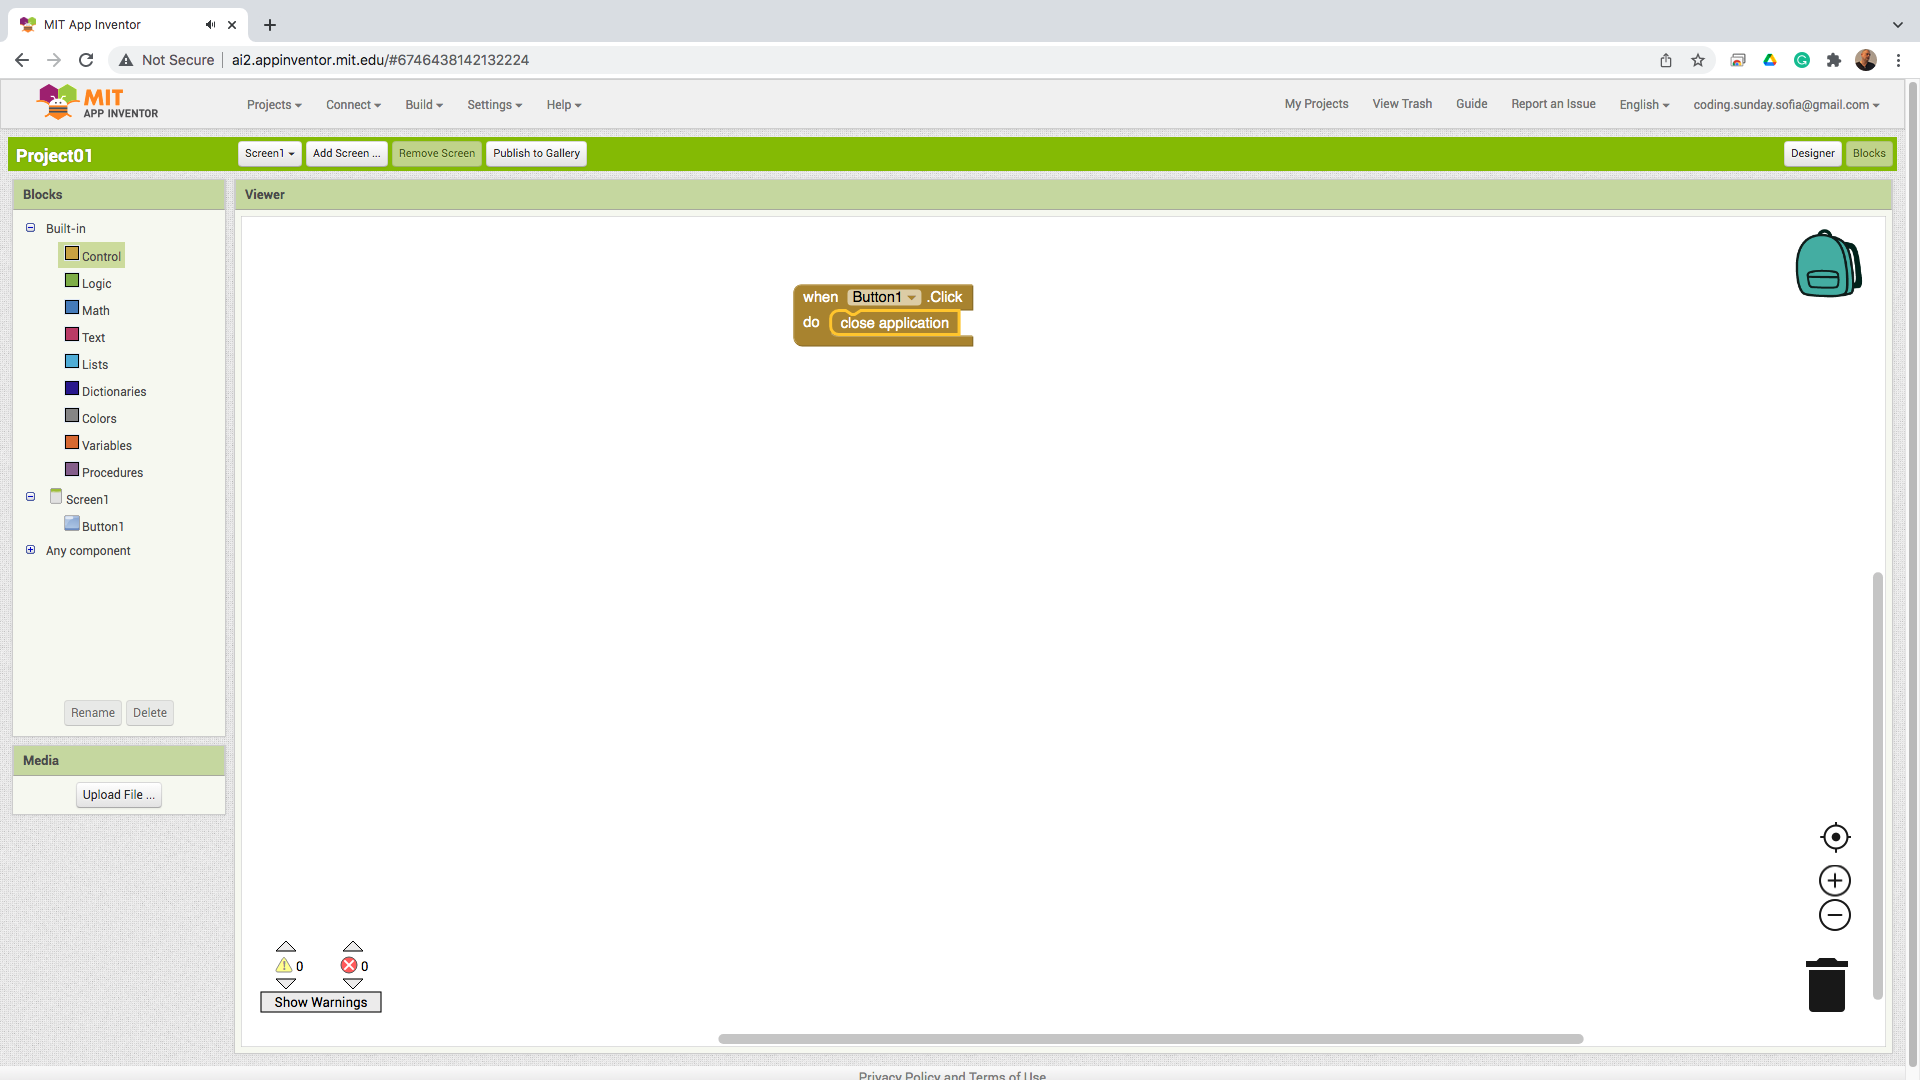
\includegraphics[width=1.0\linewidth,height=0.5\linewidth]{fig010037.png}
   \caption{Close application on button click}
\label{fig010037}
\end{figure}

After the graphical programming interface is designed and the desired instructions are arranged, the code is compiled, and the complete installation package for the written program is built (Fig. \ref{fig010038}).

\begin{figure}[H]
   \centering
   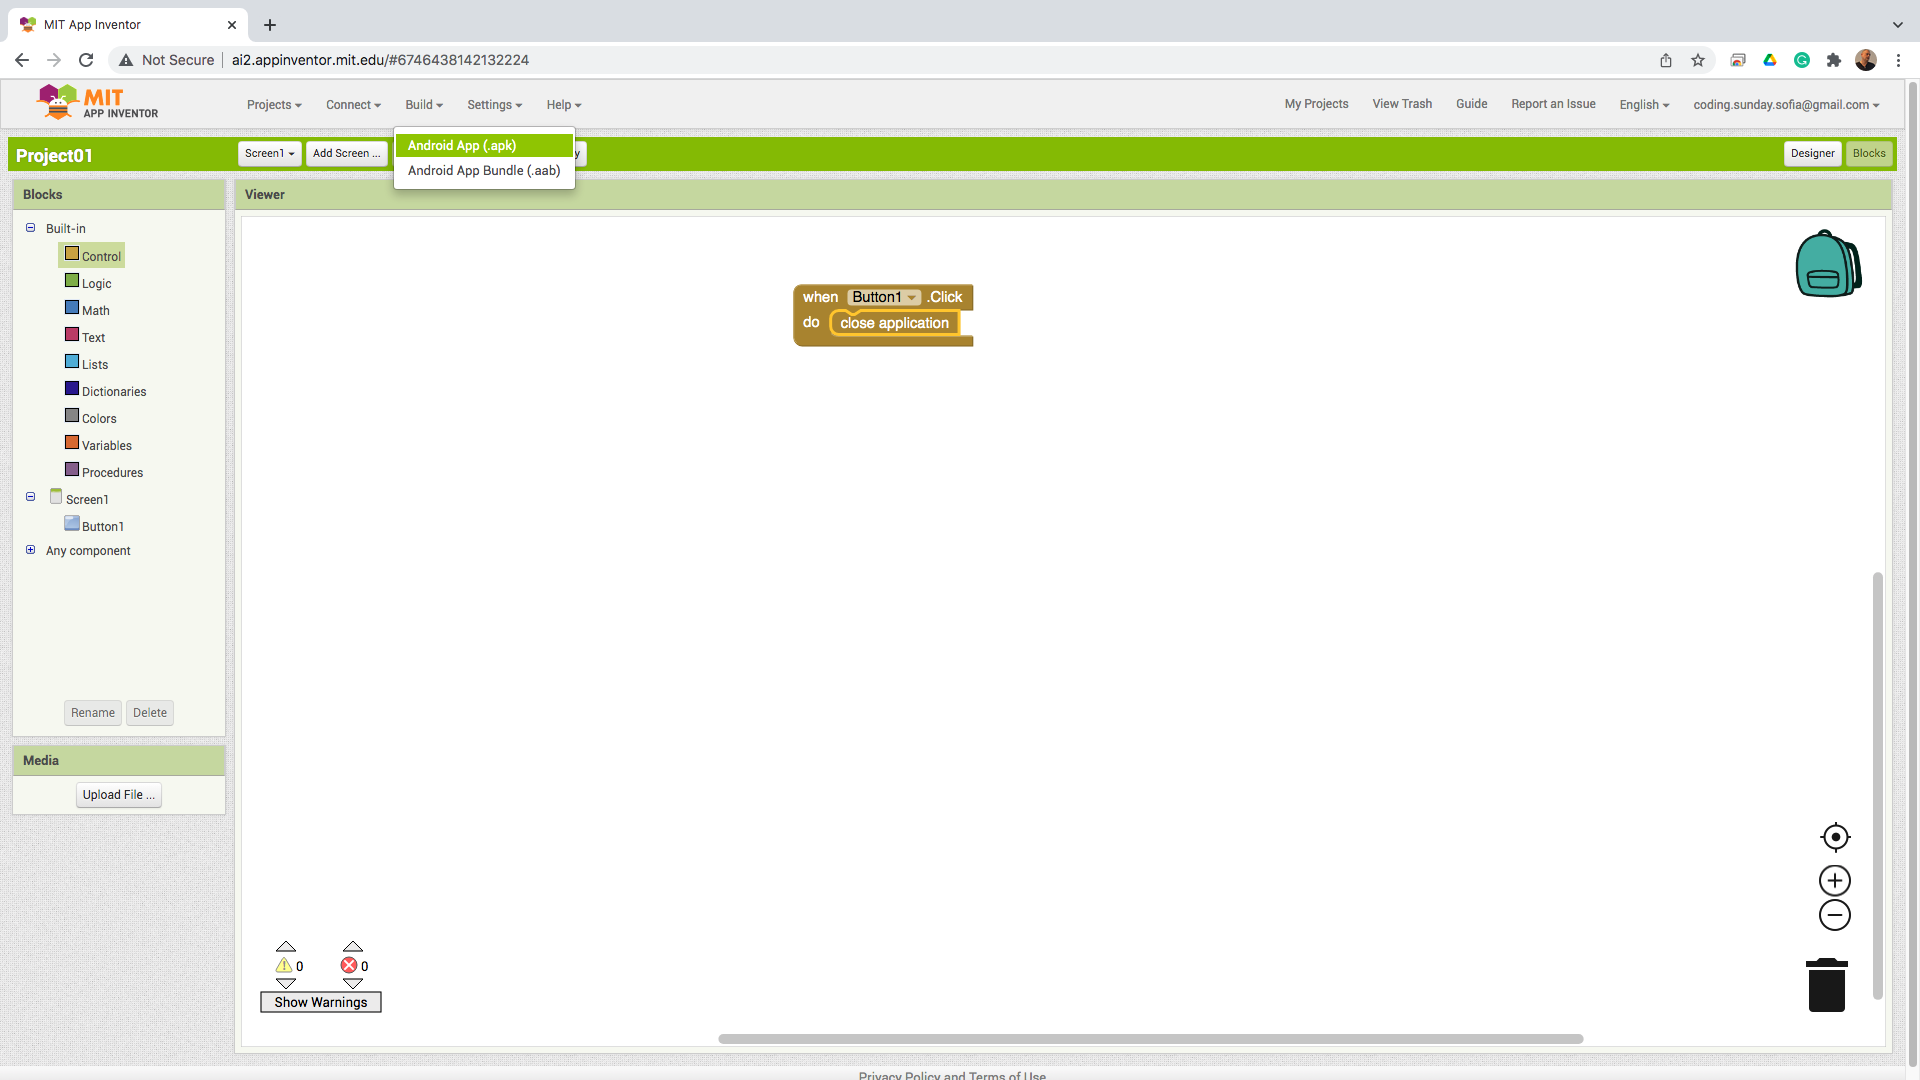
\includegraphics[width=1.0\linewidth,height=0.5\linewidth]{fig010038.png}
   \caption{Mobile App Build Menu}
\label{fig010038}
\end{figure}

A fundamental difference between Scratch and App Inventor is that the result of the execution of the programming instructions in Scratch is visible in the workspace of the programming environment itself, while in App Inventor, the installation package of the program is compiled in the cloud structure. It must be downloaded and installed on a mobile device. Compiling and building the installation package requires a particular computing time, visualized as a progress bar (Fig. \ref{fig010039}).

\begin{figure}[H]
   \centering
   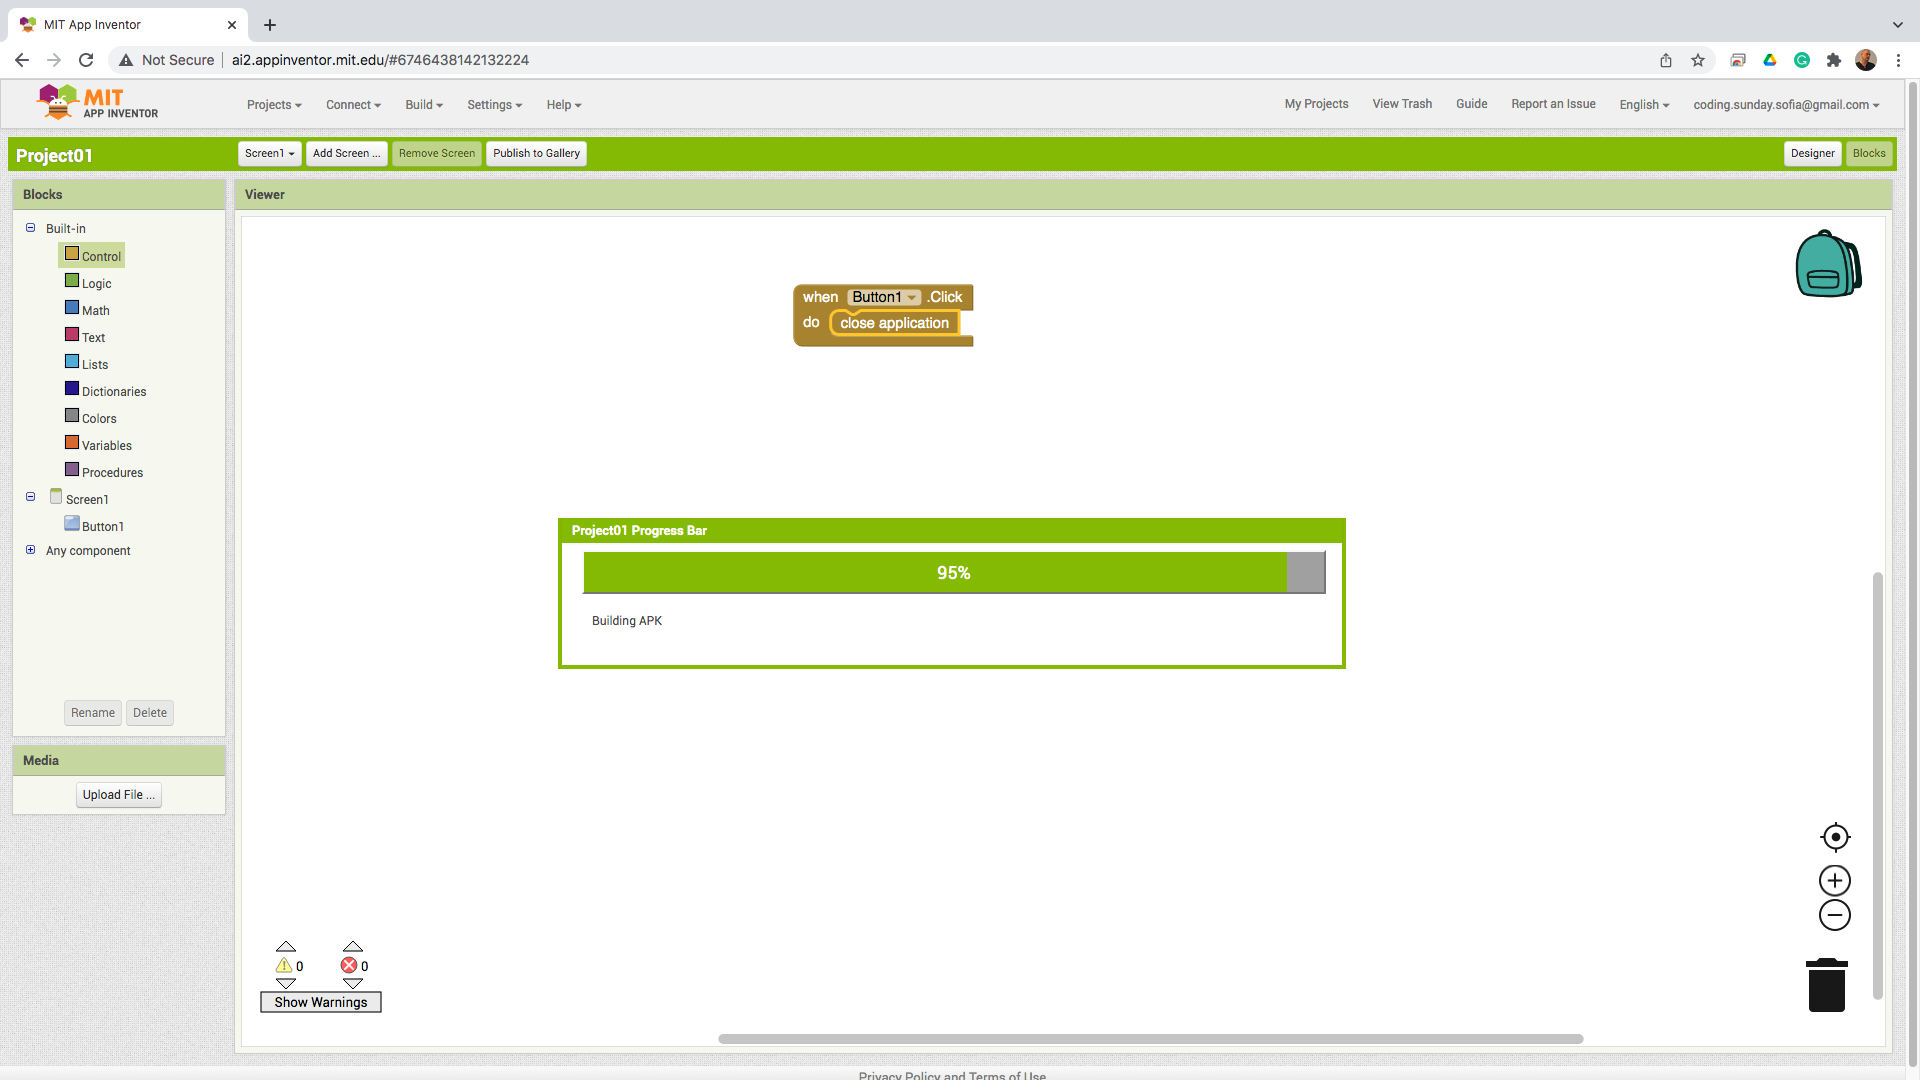
\includegraphics[width=1.0\linewidth,height=0.5\linewidth]{fig010039.png}
   \caption{App build progress}
\label{fig010039}
\end{figure}

After the project is compiled and the installation package is created, the programming environment offers a QR code (Fig. \ref{fig010040}) through which the installation package can be downloaded from the mobile device (phone or tablet).

\begin{figure}[H]
   \centering
   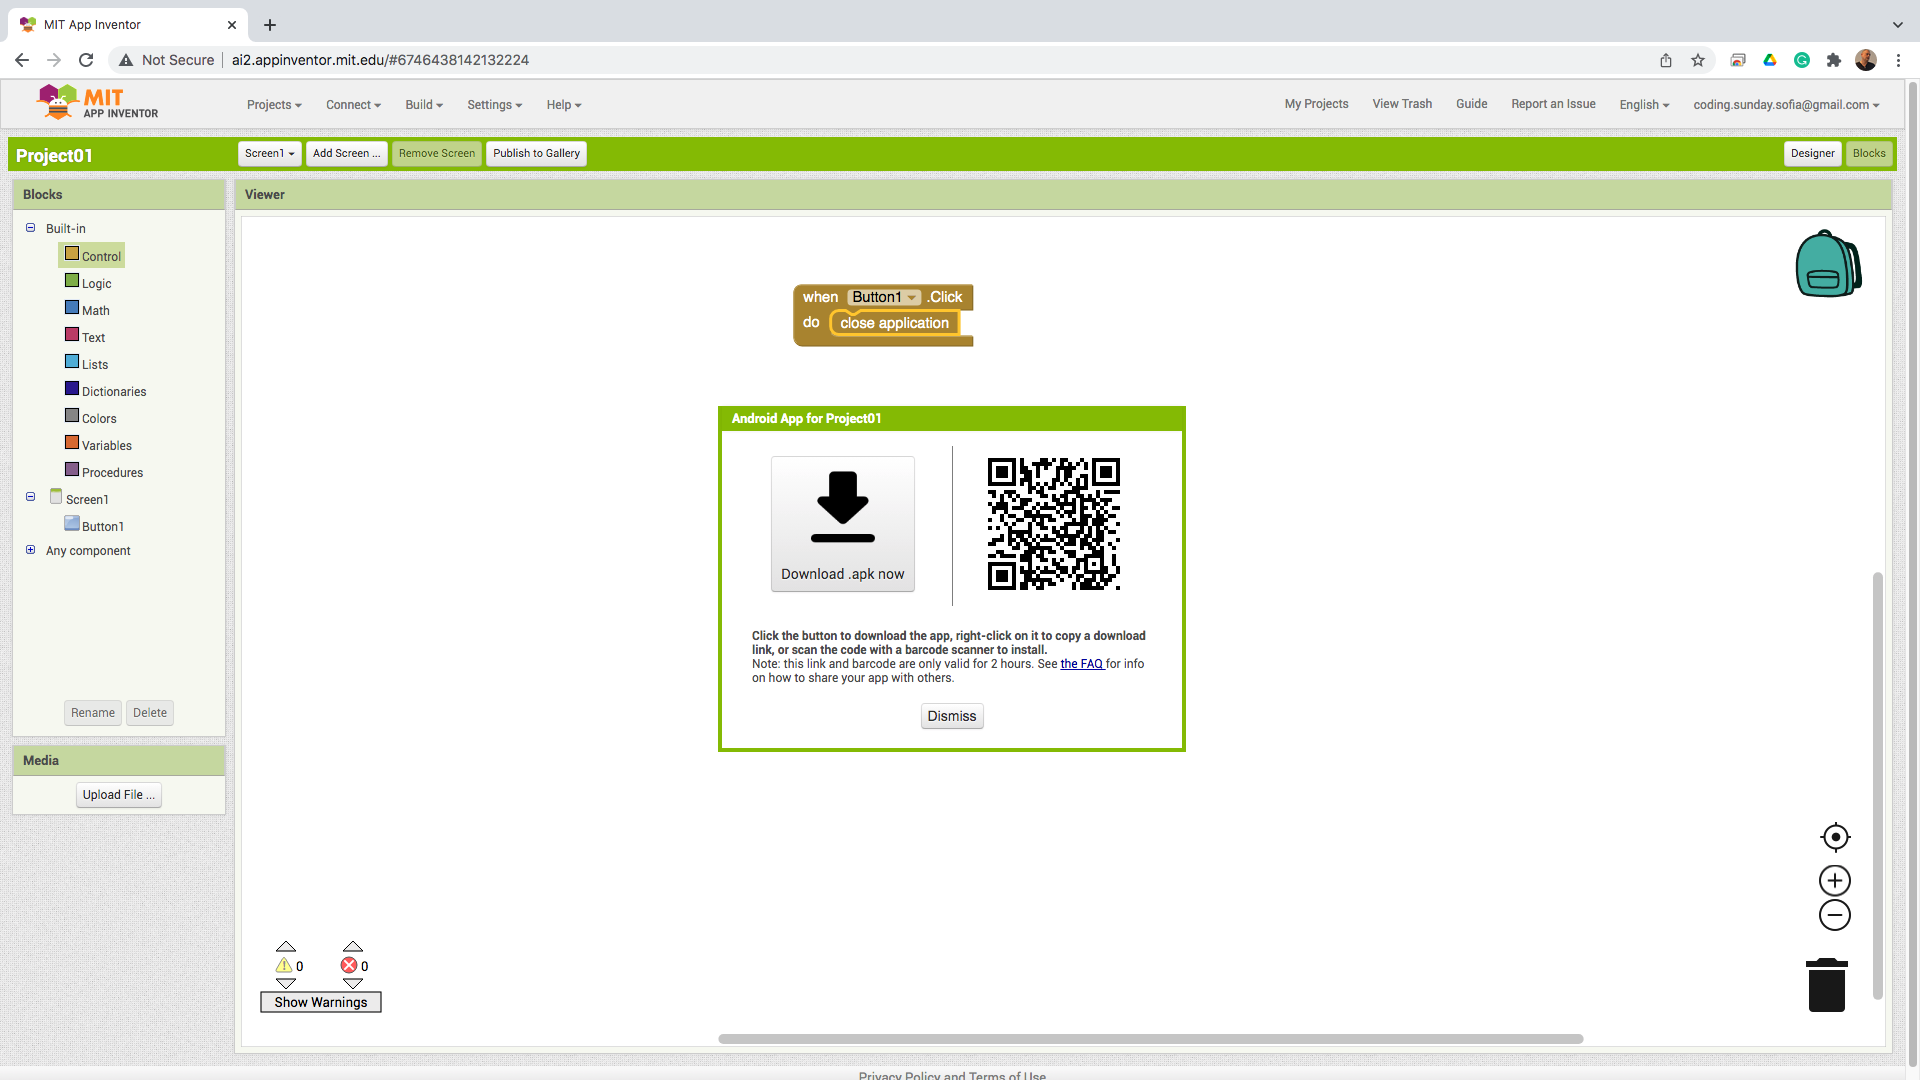
\includegraphics[width=1.0\linewidth,height=0.5\linewidth]{fig010040.png}
   \caption{Code for installing the application on a mobile device}
\label{fig010040}
\end{figure}

The creators of the App Inventor programming environment have foreseen the possibility of a faster and easier installation of the written programs through a specially created application (MIT AI2 Companion), which will take over the communication with the cloud infrastructure of App Inventor (Fig. \ref{fig010041}). The application is available on Google Play and requires no special skills to be installed on a personal mobile device.

\begin{figure}[H]
   \centering
   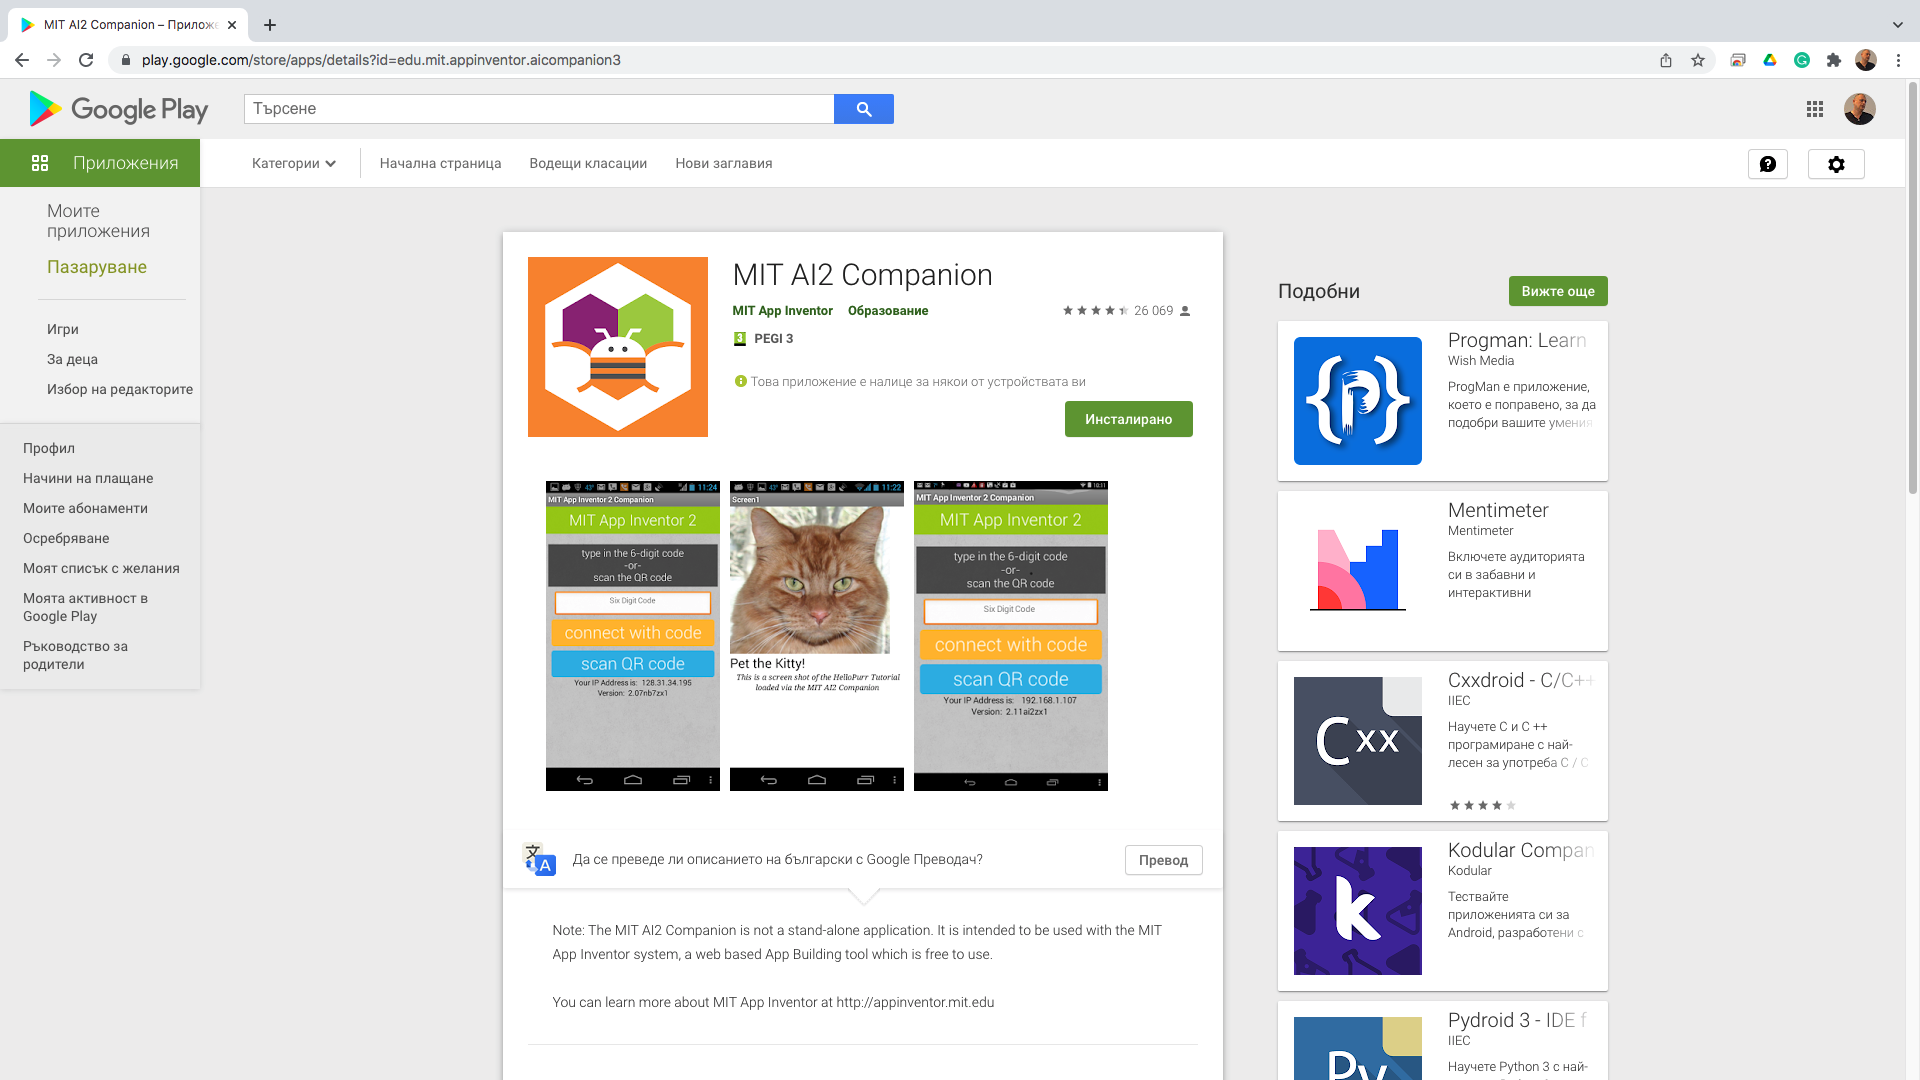
\includegraphics[width=1.0\linewidth,height=0.5\linewidth]{fig010041.png}
   \caption{Mobile application for managing compiled projects}
\label{fig010041}
\end{figure}

When the MIT AI2 Companion is started, the application gives two options to download the already written programs (Fig. \ref{fig010042}). One option is entering a code, and the second is scanning a QR code. Scanning the QR code is significantly faster and more convenient (Fig. \ref{fig010043}). Since the installation package is an executable file, the Android operating system warns that such files may be dangerous (Fig. \ref{fig010044}).

\begin{figure}[H]
   \begin{subfigure}{0.31\textwidth}
   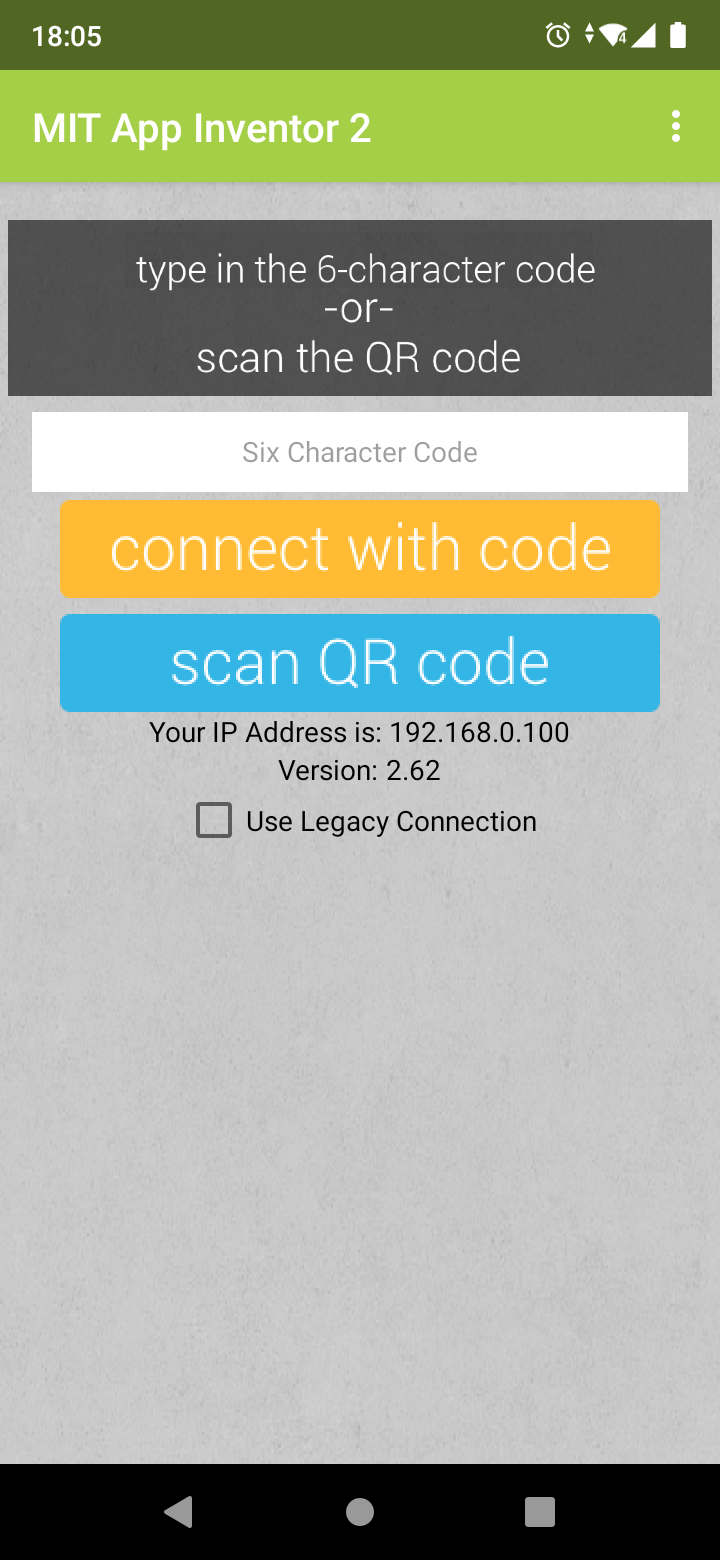
\includegraphics[width=\linewidth]{fig010042.png}
   \subcaption{\tiny Installation Selection}
   \label{fig010042}
   \end{subfigure}
   \begin{subfigure}{0.31\textwidth}
   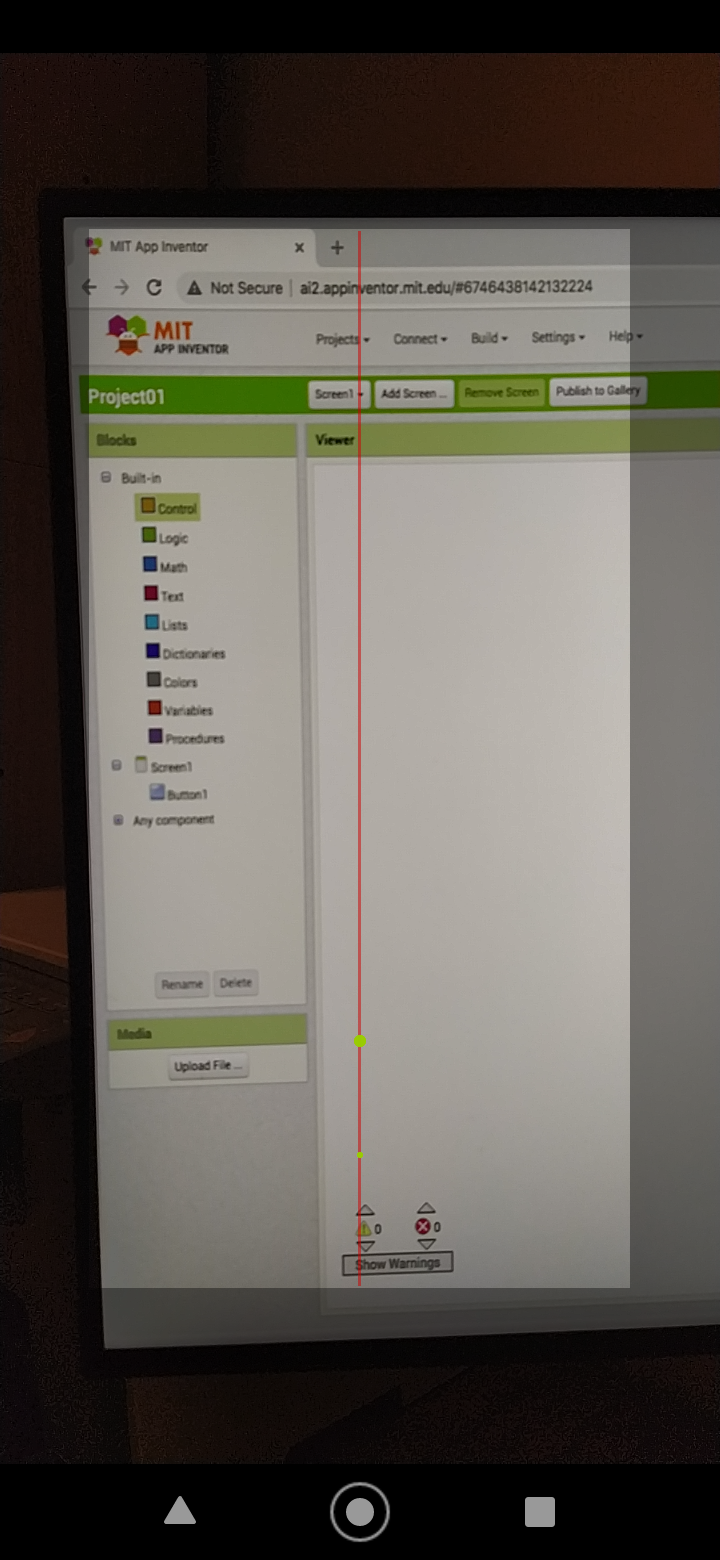
\includegraphics[width=\linewidth]{fig010043.png}
   \subcaption{\tiny Code Scan}
   \label{fig010043}
   \end{subfigure}
   \begin{subfigure}{0.31\textwidth}
   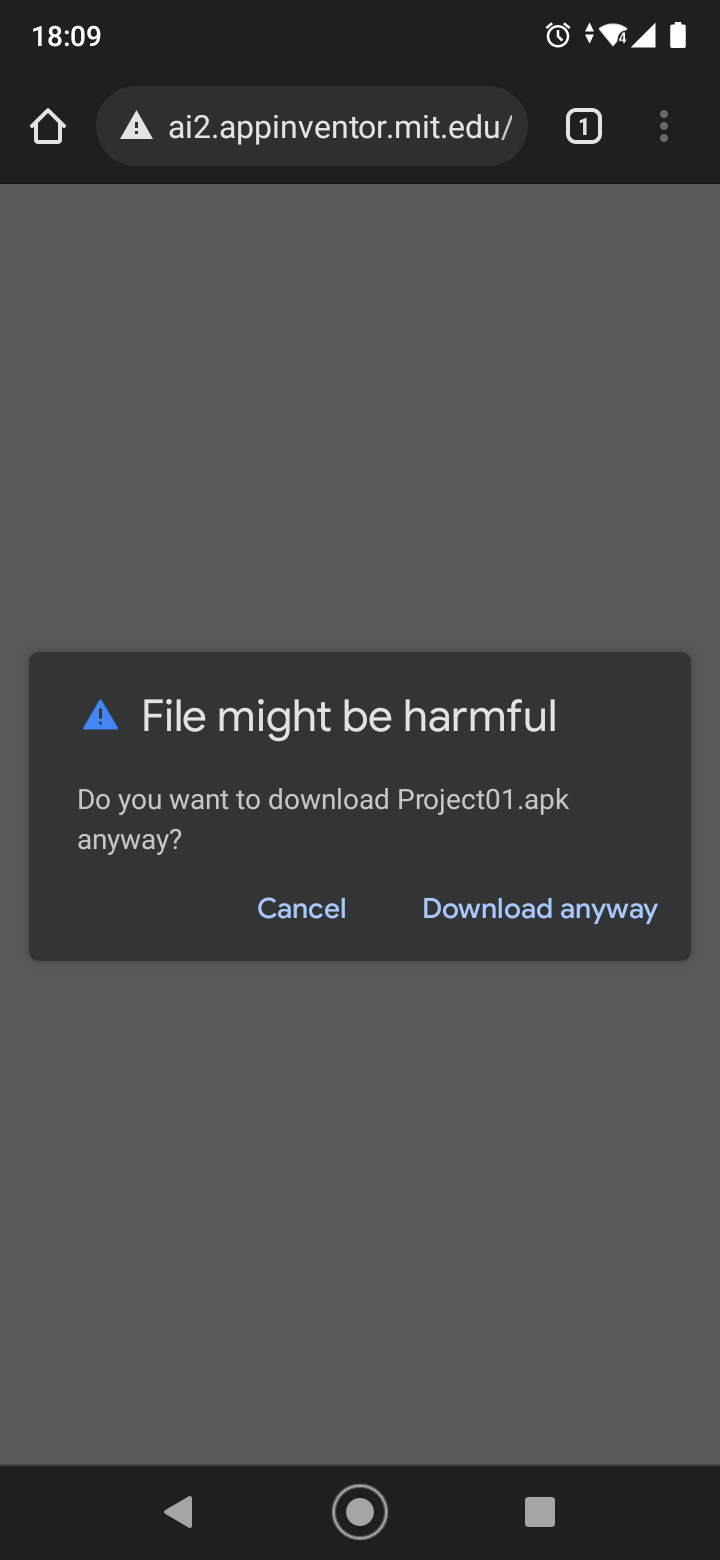
\includegraphics[width=\linewidth]{fig010044.png}
   \subcaption{\tiny Download File}
   \label{fig010044}
   \end{subfigure}
   \caption{Install via QR code}
\end{figure}

After downloading the installation package, the operating system issues a message about the successful operation of recording the installer (Fig. \ref{fig010045}). The user must select the installation package and activate it. This prompts you to ask if you want to install the program in the downloaded file (Fig. \ref{fig010046}). Although we know exactly how the installation file was created, the operating system perceives it as a program developed by an unverified developer. For this reason, it asks the user again if he wants to do the installation (Fig. \ref{fig010047}).

\begin{figure}[H]
   \begin{subfigure}{0.31\textwidth}
   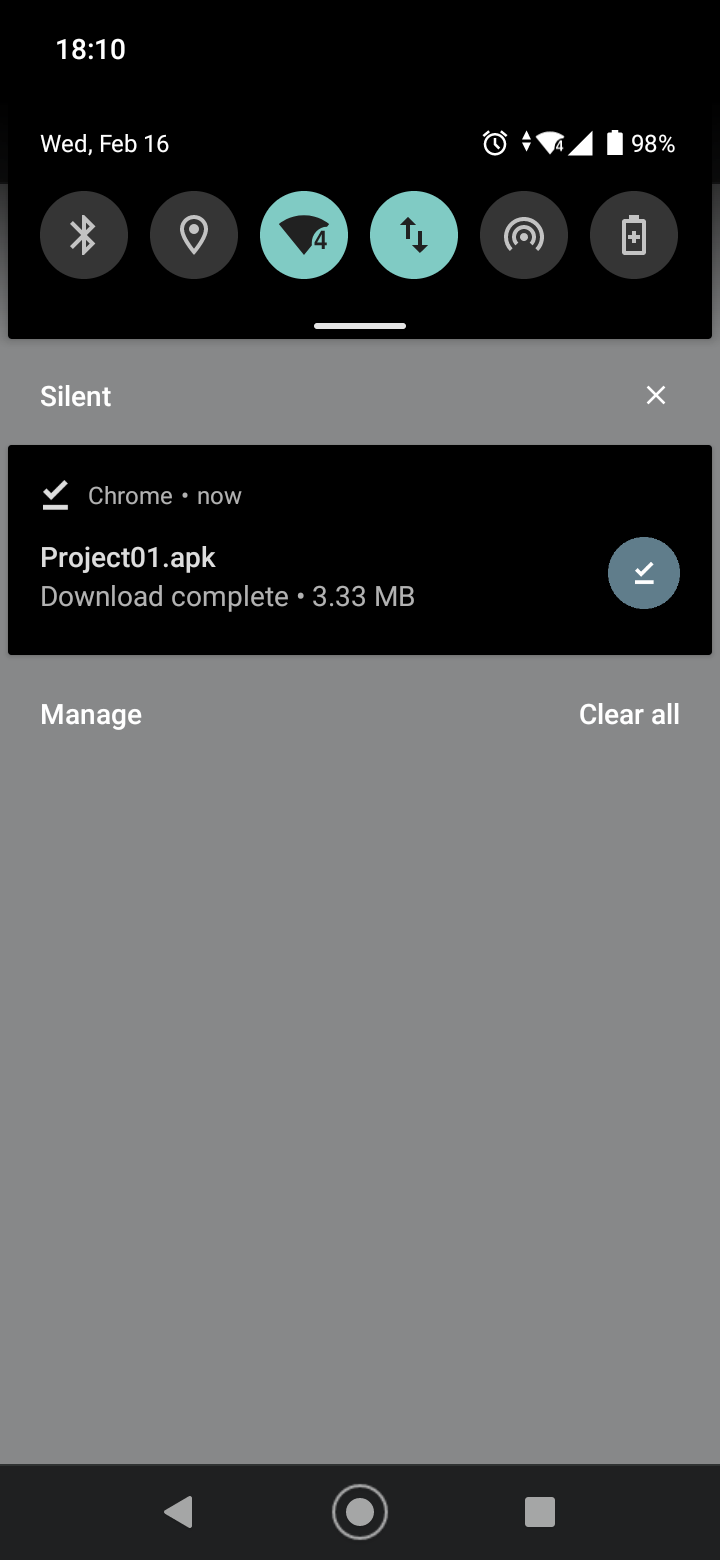
\includegraphics[width=\linewidth]{fig010045.png}
   \subcaption{\tiny File Downloaded}
   \label{fig010045}
   \end{subfigure}
   \begin{subfigure}{0.31\textwidth}
   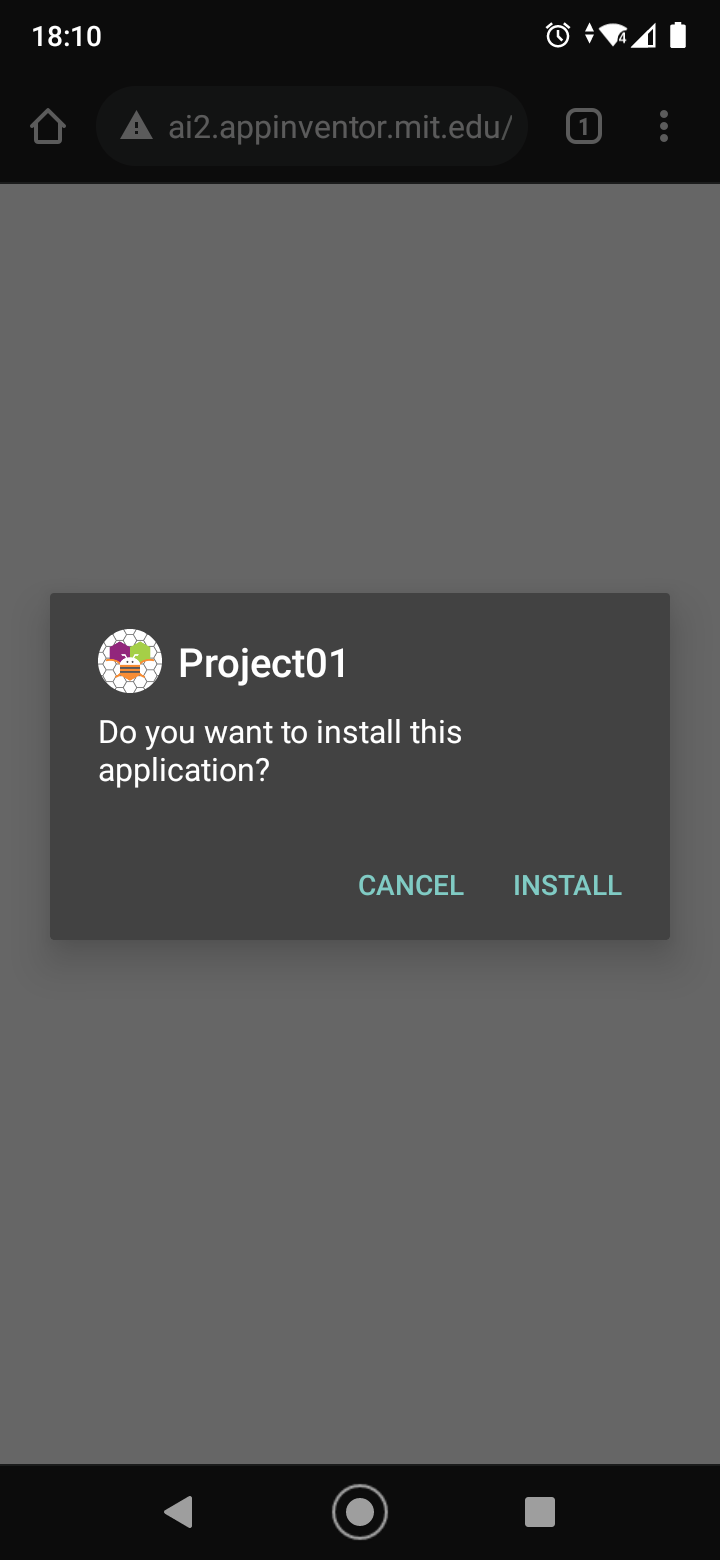
\includegraphics[width=\linewidth]{fig010046.png}
   \subcaption{\tiny Choose to install}
   \label{fig010046}
   \end{subfigure}
   \begin{subfigure}{0.31\textwidth}
   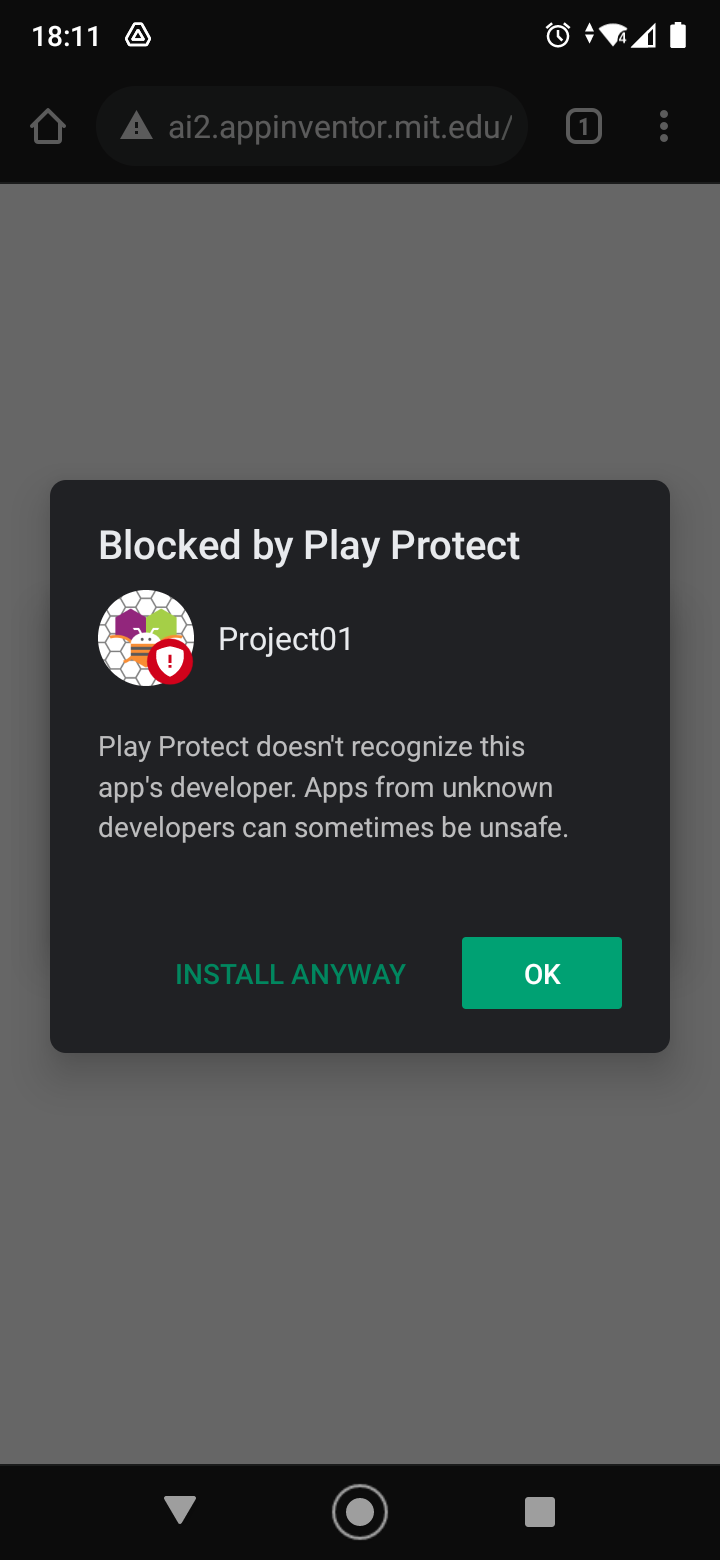
\includegraphics[width=\linewidth]{fig010047.png}
   \subcaption{\tiny Installation Confirmation}
   \label{fig010047}
   \end{subfigure}
   \caption{Installation on the mobile device}
\end{figure}

"Install Anyway" is selected, and the written program is installed on the mobile device. The installation process ends with a window prompting to start the newly installed program (Fig. \ref{fig010048}). To check the operation of the written code, it is enough to press the visualized button in the upper left corner (Fig. \ref{fig010049}). This action results in closing the window and visualizing the virtual wallpaper (Fig. \ref{fig010049}).

\begin{figure}[H]
   \begin{subfigure}{0.31\textwidth}
   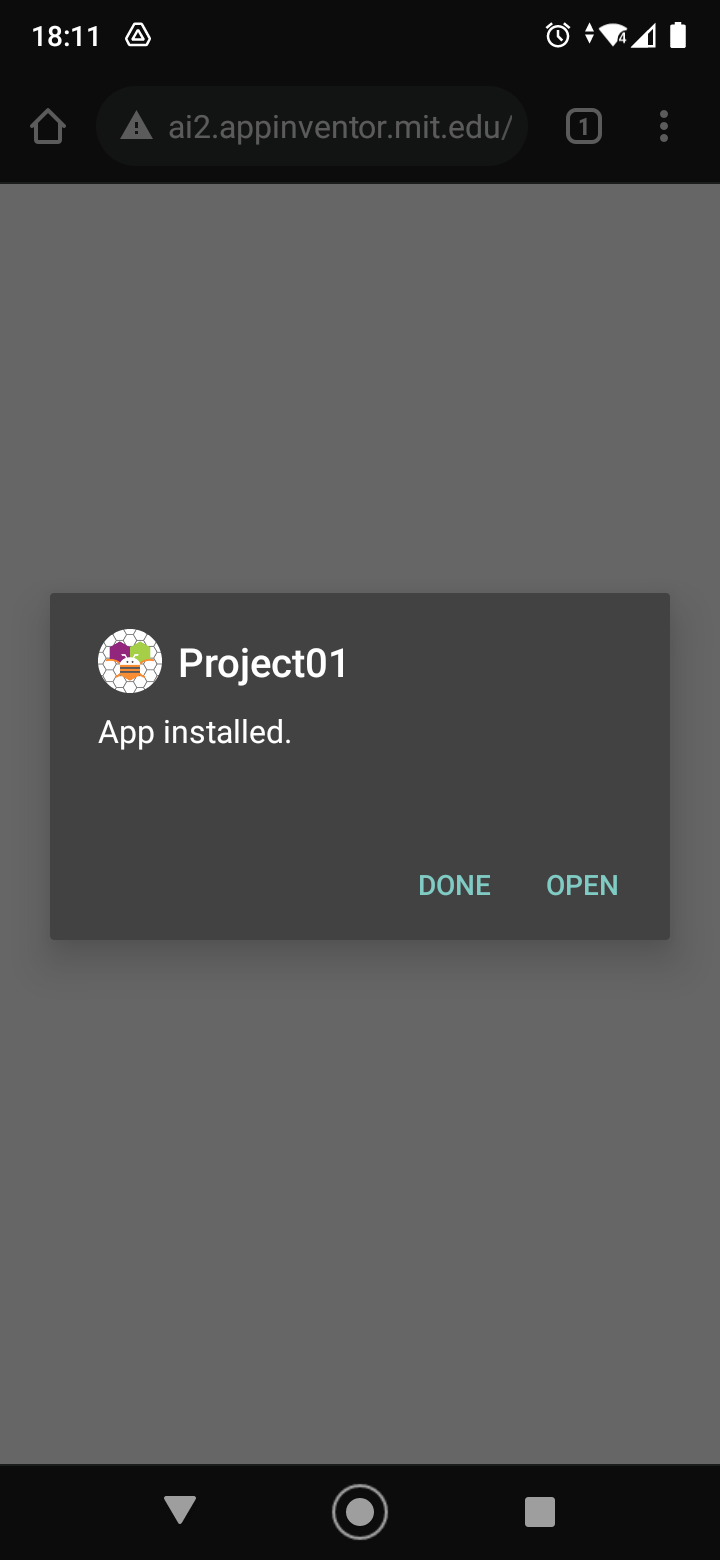
\includegraphics[width=\linewidth]{fig010048.png}
   \subcaption{\tiny Launch}
   \label{fig010048}
   \end{subfigure}
   \begin{subfigure}{0.31\textwidth}
   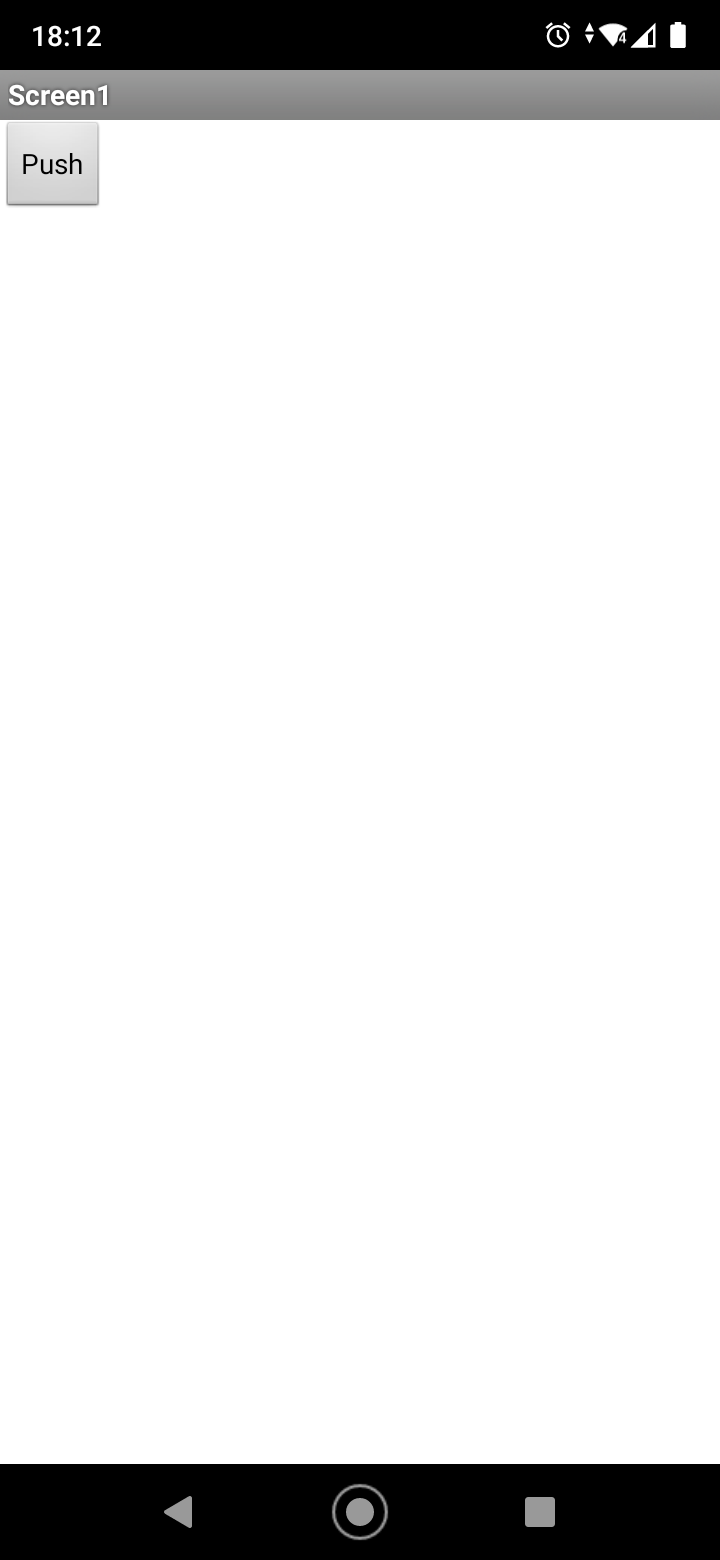
\includegraphics[width=\linewidth]{fig010049.png}
   \subcaption{\tiny Button Selection}
   \label{fig010049}
   \end{subfigure}
   \begin{subfigure}{0.31\textwidth}
   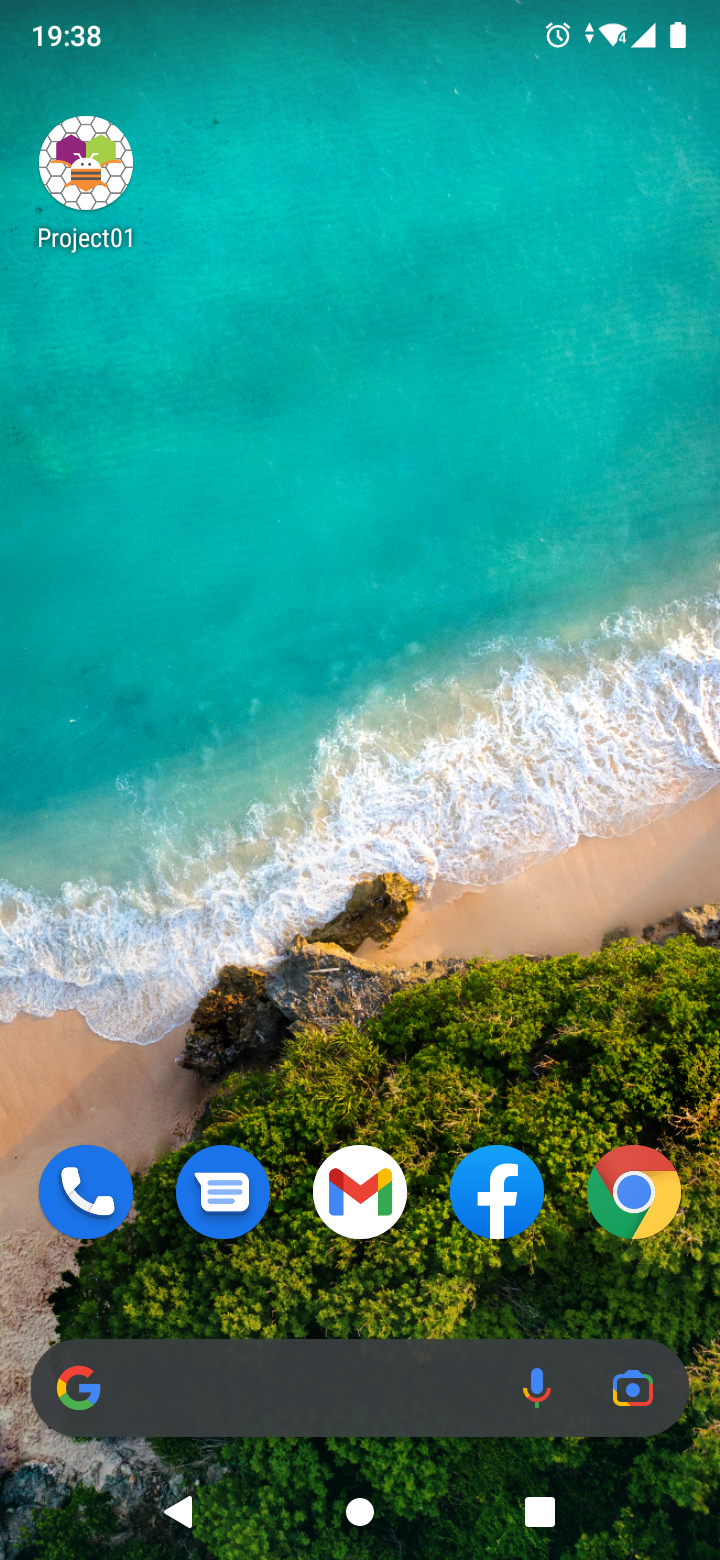
\includegraphics[width=\linewidth]{fig010050.png}
   \subcaption{\tiny Closed App}
   \label{fig010050}
   \end{subfigure}
   \caption{Working with the application}
\end{figure}

With App Inventor, the most fascinating part is that the developed programs become available on mobile devices, and the person who creates them can show their work even when they are not in front of the computer or do not have Internet connectivity.
